% % % % % % % % % % % % % % % % % % % % % % % % % % % % % % % % % % % % % % % 
%																						%
%	LaTeX-Vorlage für Abschlussarbeiten 														%
%																						%
%		Diese Vorlage für Abschlussarbeiten wurde im Auftrag des Instituts für Papierfabrikation und mechanische Verfahrenstechnik der TU Darmstadt (PMV)	für die Lehrveranstaltung "Wissenschaftliches Arbeiten und Schreiben für Maschinenbau-Studierende"   %
%		erstellt. Als Basis dienten die LaTeX-Vorlagen der Physik der TU % Darmstadt sowie von Prof. Dr.-Ing. Oberlack, Maschinenbau, TU Darmstadt. 																	     %
%		Vor der Verwendung wird die Lektüre des Skripts zur Veranstaltung "Wissenschaftliches Arbeiten       %
%		und Schreiben für Maschinenbau-Studierende" empfohlen.									  %
%		Bei Fragen, Anregungen und Kritik wenden Sie sich bitte an ckuhn@spz.tu-darmstadt.de			%
%																						%
% % % % % % % % % % % % % % % % % % % % % % % % % % % % % % % % % % % % % % %

\documentclass[accentcolor=tud7a, bigchapter, colorbacktitle,toc=listof, toc=bibnumbered, parskip=off, 11pt, a4paper]{tudreport}

% Einfügen der Header-Datei welche die Dokumentenpräambel enthält, in der die verwendeten Zusatz-Packages geladen und konfiguriert werden
		
	% % % % % % % % % % % % % % % % % % % % % % % % 
	%													  %
	% 	Definition der Dokumentenklasse und ihrer Einstellungen		%
	%													  %
	% % % % % % % % % % % % % % % % % % % % % % % %
	
	% Die verwendete TUD-Design-Klasse tudreport setzt auf der KOMA-Script-Klasse scrreprt auf und implementiert die Vorgaben des Corporate Design Handbuchs der TU Darmstadt. 
	% scrreprt bringt einige Voreinstellungen mit sich: 
	% 11pt, a4paper, abstractoff, bigheadings, final, footnosepline, headnosepline, nochapterprefix, onecolumn, oneside, openany, parindent, tablecaptionbelow und titlepage. 
	% Details zu diesen Voreinstellungen können der Dokumentation des KOMA-Scripts entnommen werden. Im folgenden werden lediglich Optionen definiert, welche von den Voreinstellungen abweichen oder durch die Klasse tudreport definiert werden.
	
	%\documentclass[accentcolor=tud7a, bigchapter, colorbacktitle,toc=listof, toc=bibnumbered, parskip=off, 11pt, a4paper]{tudreport}
	
	%TUD-Design Optionen
	% accentcolor, bigchapter & colorbacktitle: siehe Dokumentation zum TUD-Design
	% ACHTUNG: die accentcolor Einstellung entfaltet derzeit keine Wirkung, da am Ende dieser Datei eine modifizierte Identbar für die Kopfzeile eingebunden wird (um die zweifarbige Identbar in der Kopfzeile zu realisieren). Für eine einfarbige Identbar kann der Input-Befehl auskommentiert werden, wodurch accentcolor wieder seine Wirkung zurück erlangt.
	
	%KOMA-Script Optionen (werden durchgereicht an scrreprt)
	% 11pt								% setzt die Schriftgröße auf 11pt
	% a4paper							% Seitengröße DIN A4
	% toc=listof 							% sorgt dafür, dass die Verzeichnisse der Gleitumgebungen, z.B. das Abbildungs- und das Tabellenverzeichnis, im Inhaltsverzeichnis erscheinen (alternativ mit Nummerierung im Inhaltsverzeichnis: listofnumbered)
	% toc=bibnumbered  					% sorgt dafür, dass das Literaturverzeichnis einen nummerierten Eintrag im Inhaltsverzeichnis erhält (alternative Einstellung: ohne Nummerierung im Inhaltsverzeichnis mit Befehl bib)
	% parskip = full 						% setzt den Zeilenabstand auf eine volle Zeile und unterbindet den Erstzeileneinzug eines neuen Absatzes
	
	
	% % % % % % % % % % % % % % % % % % % % % % % % % % % % % % % % %
	%																		    %
	%	 Laden von Paketen zur Erweiterung des Funktionsumfangs						    %
	% 	Die Dokumentationen der verwendeten Pakete befinden im Unterordner ASFDKFAKDF	%
	%																		    %
	% % % % % % % % % % % % % % % % % % % % % % % % % % % % % % % % % 
	%\usepackage[ngerman]{babel}		
	% Das Babel-Paket passt LaTeX für die Verwendung der deutschen Sprache (neue deutsche Rechtschreibung) an.
	\usepackage[utf8]{inputenc} 
	% Eingabekodierung auf utf8 setzen (ermöglicht die direkte Verwendung von ä, ö, ü und ß beim Schreiben des Textes). Die Speicherung der TeX-Dateien muss im LaTeX-Editor entsprechend dieser Codierung erfolgen!
	\usepackage[T1]{fontenc}
	% Font-Encoding auf T1 setzen (stellt sicher dass ä, ö, ü und ß später im PDF gefunden werden)
	\usepackage{geometry}
	% Das Geometry-Paket erleichtert die Festlegung des Seitenlayouts und ermöglicht die einfache Verwendung mehrerer Layout-Umgebungen
	\usepackage{setspace}
	% Ermöglicht einfache Kontrolle über den Zeilenabstand mittels spacing-Befehlen und spacing-Umgebungen
	\usepackage{graphicx}		
	% ermöglicht die Einbindung von Grafiken und Bildern
	\usepackage{hyperref}											
	% erzeugt in der PDF-Ausgabe klickbare Links für Überschriften, etc. und setzt Lesezeichen welche beispielsweise in Adobe Reader genutzt werden können
	\usepackage{booktabs}											
	% ermöglicht die Gestaltung professioneller Tabellen
	\usepackage{longtable}
	% ermöglicht die Gestaltung von Tabellen, welche mehrere Seiten umfassen, z.B. Symbolverzeichnisse (kompatibel zu booktabs)
	\usepackage[section]{placeins}									
	% verhindert dass Gleitumgebungen über Section-Grenzen hinaus wandern, führt außerdem den Befehl \FloatBarrier ein
	\usepackage{siunitx}
	% Paket zur korrekten und einheitlichen Darstellung von Zahlen und Einheiten (Verwendung siehe Dokumenation)
	\usepackage[babel, german=quotes]{csquotes} 
	\RequirePackage[backend=biber, style=ieee, citestyle=ieee, bibstyle=ieee, firstinits=true, maxnames=3%authortitle-icomp
	]{biblatex} %backend=biber
	\bibliography{main}
	% Einstellung der Anführungszeichen bei Zitaten
	%\usepackage[backend=biber, style=numeric-comp, bibstyle=numeric, citestyle=numeric]{biblatex}
	%\addbibresource{bibliography.bib}
	\usepackage{graphicx}
	%\usepackage{subfigure}
	\usepackage{caption}
	\usepackage{subfigure}
	\usepackage{yhmath}
	\usepackage{amsmath}
	\usepackage{listings} 
	\usepackage[justification = centering]{caption}
	%	\usepackage{amssymb}
	\usepackage{color}
	\newcommand{\todo}[1]{\textcolor{red}{@TODO: #1}}
	\newcommand{\plusminus}[2]{$\pm$}
	\usepackage[mathcal]{eucal}
	\usepackage{pgfplots}
	\pgfplotsset{compat=1.12} %width=7cm,
	\usepackage{pgfplotstable}
	%	%\usepgfplotslibrary{external} 
	%	%\usepgfplotslibrary[external]
	%	%\usetikzlibrary{pgfplots.external}
	%	%\usetikzlibrary[pgfplots.external]
	%	%\usepgfplotslibrary{external}
	%	%\tikzexternalize
	%	%\tikzset{external/force remake}
	%	
	\usepackage{multirow}
	\usepackage{rotating}
	\newcommand{\argmax}{\operatornamewithlimits{argmax}}
	
	
	% biblatex ist ein Paket zur Ausgabe und Formatierung von Zitaten und von Literaturverzeichnissen
	%backend=biber		% Einstellung für die Verwendung von biber als Bibliographie-Prozessor
	%style=numeric-comp		% Einstellung des
	%bibstyle=numeric			% Einstellung des Bibliographie-Stils
	%citestyle=numeric		% Einstellung des Zitierstils
	\usepackage[
	nomain,
	xindy,
	nonumberlist, 			% keine Anzeige von Seitenzahlen der Einträge im Abkürzungs-/Symbolverzeichnis
	nogroupskip, 			% keine Gruppierung der Einträge nach Anfangsbuchstaben & keine zusätzlicher vertikaler Abstand bei Änderung des Anfangsbuchstabens
	acronym, 			% ein Abkürzungsverzeichnis erstellen
	toc, 					% Einträge im Inhaltsverzeichnis für das Abkürzungs- und Symbolverzeichnis
	translate=babel, 		% Übersetzung von Überschriften, etc. ins Deutsche
	]{glossaries}			% Paket zur Erstellung von Abkürzungs-, Symbolverzeichnissen, etc.
	\usepackage{blindtext}		% Ermögicht die einfache Verwendung von Beispieltext zu Testzwecken
	\usepackage[xindy]{imakeidx}
	\makeindex
	% weitere möglicherweise interessante Pakete: capt-of, multirow
	
	
	% % % % % % % % % % % % % % % % % % % 
	%										 %
	%	Festlegen von Einstellungen der Pakete		%
	%										 %
	% % % % % % % % % % % % % % % % % % % 
	
	\geometry{top=2.5cm, left=2.5cm, right=2.5cm, bottom=2cm}			
	% Definition der Seitenränder
	\graphicspath{{img/}}															% legt Unterverzeichnisse fest in denen \includegraphics standardmäßig nach Bilddateien sucht
	\sisetup{
		exponent-product = \cdot,		% setzt einen Malpunkt als Trennzeichen bei der Verwendung von Exponenten
		output-decimal-marker = {,},		% setzt Komma als Dezimalzeichen (im Englischen ist es ein Punkt)
		per-mode = symbol,			% legt fest, dass Einheiten im Nenner mit einem Bruchstrich statt mit negativen Exponenten dargestellt werden
		bracket-unit-denominator = false,	% mehrere Einheiten im Nenner werden nicht durch eine Klammer umschlossen
		range-phrase = ~--~,			% bei Verwendung von \SIrange wird ein Bindestrich zwischen den beiden Zahlen verwendet
		number-unit-product = \text{~},	% legt den Abstand zwischen Zahl und Einheit fest
		detect-all,					% hiermit werden Veränderungen der Schrift auch bei der Darstellung der Zahlen und Einheiten berücksichtigt
		list-final-separator = ~und~,		% Übersetzung
		list-pair-separator = ~und~,		% Übersetzung
	}
	\urlstyle{same}
	\hypersetup{ %
		colorlinks = true,		% true: stellt Verknüpfungen wie Links, Zitate und Verweise farbig dar, false: rahmt Links, Zitate und Verweise in einen farbigen Rahmen ein
		urlcolor = darkgray,		% Schriftfarbe für URLs
		citecolor = darkgray,		% Schriftfarbe für Zitate
		pdfborder = 0 0 1,		% legt Rahmen fest, sofern verwendet
		linkbordercolor = white,	% Rahmenfarbe bei Verweisen (white = transparent bei weißem Hintergrund)
		urlbordercolor = black,		% Rahmenfarbe bei URLs
		citebordercolor = white,		% Rahmenfarbe bei Zitaten (white = transparent bei weißem Hintergrund)
		bookmarksopen = false,		% legt fest ob die Lesezeichenleiste beim Öffnen des PDFs expandiert ist oder nicht
		bookmarksnumbered = true,	% legt fest ob die Kapitelnummern in den Lesezeichenbaum übernommen werden
	}
	
	% % % % % % % % % % % % % % % % % % %
	%										 %
	% 	Anpassung des Literaturverzeichnisses		%
	%										 %
	% % % % % % % % % % % % % % % % % % % 
	
	% läd die Literaturdatenbank aus dem aktuellen Arbeitsverzeichnis
	\ExecuteBibliographyOptions{%
		url = false,
		%dashed=false			%in Bibliographie-Stilen, welche das Literaturverzeichnis nach Autorennamen sortieren werden bei setzen der Einstellung auf true bei mehreren Quellen eines Autors die Einträge untereinander gruppiert und der Autorenname durch einen Strich ersetzt
		bibencoding=utf8, % wenn .bib in utf8, sonst ascii
		bibwarn=true, % Warnung bei fehlerhafter bib-Datei
		sorting=none % gibt Einträge im Literaturverzeichnis in der Reihenfolge aus, in der sie zitiert wurden	
	}%
	
	\DefineBibliographyStrings{ngerman}{%
		bibliography={Literaturverzeichnis},			% setzt die Überschrift des Literaturverzeichnis
		urlseen          = {Zugriff\addcolon}				% ändert die Beschriftung des Datums bei URLs von "besucht am" auf "Zugriff:"
	}
	
	\DeclareNameAlias{default}{last-first}  			
	%Im Literaturverzeichnis folgt die Darstellung der Autorennamen der Darstellung Nachname, Vorname (abhängig vom Stil, muss dies angepasst werden um die Effekt zu erhalten, siehe: http://projekte.dante.de/DanteFAQ/BiblatexReihenfolgeAutoren)
	\renewcommand*{\mkbibnamelast}[1]{\textsc{#1}}		
	%Setzen des Nachnamens des Autors in Kapitälchenschrift
	
	
	% % % % % % % % % %% % % % % % % % % % % % % % % 
	%												              %
	%	Neu-Definitionen und Änderungen bestehender Befehle		%
	%													      %
	% % % % % % % % % % % % % % % % % % % % % % % % % 
	
	% Neudefinition der Itemize-Umgebung um die Abstände zwischen einzelnen Stichpunkten von Aufzählungen zu Verringern
	\let\olditemize\itemize
	\renewcommand{\itemize}{
		\olditemize
		\itemsep4pt
	}
	
	% Neudefinition der Enumerate-Umgebung um die Abstände zwischen einzelnen Stichpunkten von Aufzählungen zu Verringern
	\let\oldenumerate\enumerate
	\renewcommand{\enumerate}{
		\oldenumerate
		\itemsep4pt
	}
	
	%\addto\extrasngerman{\def\figureautorefname{Abb.}}							
	% legt fest, dass bei Verweis auf eine Abbildung im Text, das Wort Abbildung mit Abb. abgekürzt wird
	%\addto\extrasngerman{\def\tableautorefname{Tab.}}							
	% legt fest, dass bei Verweis auf eine Tabelle im Text, das Wort Tabelle mit Tab. abgekürzt wird
	
	
	% Definition der Umgebung bibeinzug für manuelle Erstellung eines Eintrags des Literaturverzeichnisses
	\newenvironment{bibeinzug}{\hangindent=1cm}{\par}
	
	% Definition des Befehls Bibzahl für manuelle Erstellung eines nummerierten Eintrags im Literaturverzeichnis
	\newcommand{\bibzahl}[2] { %
		\begin{tabular}{p{0.75cm}p{\textwidth-1.5cm}}
			[#1] &#2
		\end{tabular}
	}	

	

% Einfügen der Datei in der Aussehen und Inhalt der Titelseite hinterlegt ist
	%\input{parts/titel}
	% Erklärungen zur korrekten Verwendung der Befehle finden sich in der TUD-Design Dokumentation
	\title{Numerical simulation of compressible flows with immersed boundaries using Discontinuous Galerkin methods}
	\subtitle{Bachelorarbeit von Simone Katharina Stange}
	\subsubtitle{\today}
	\institution{Fachbereich Maschinenbau}
	%\sponsor{Sponsorenleiste}
	%\setinstitutionlogo{}
	%\settitlepicture{}
	%\printpicturesize
	
		% HINWEIS: Mit dem hyperref-Paket lassen sich entsprechende Informationen auch als Information in der PDF-Datei hinterlegen
	
%Definitionen der Abkürzungen und Symbole einfügen
	%Ein extra Verzeichnis für Symbole erstellen
\newglossary[slg]{symbolslist}{syi}{syg}{Symbolverzeichnis}

%Den Punkt am Ende jeder Beschreibung deaktivieren
\renewcommand*{\glspostdescription}{}

%Glossar-Befehle anschalten
\makeglossaries


%				    	    %
%%	Symbole definieren	%
%%					    %
%\newglossaryentry{symb:epsilon}{
%	name=$\varepsilon$,
%	description={Dehnung},
%	sort=epsilon, type=symbolslist
%}
%\newglossaryentry{symb:phi}{
%	name=$\varphi$,
%	description={Winkel},
%	sort=phi, type=symbolslist
%}
%\newglossaryentry{symb:E}{
%	name=E,
%	description={Elastizitätsmodul},
%	sort=E, type=symbolslist
%}
%\newglossaryentry{symb:T}{
%	name=T,
%	description={Temperatur},
%	sort=T, 
%	type=symbolslist,
%	symbol=\si{\kelvin}
%}
%\newglossaryentry{symb:sigma}{
%	name=$\sigma$,
%	description={Spannung},
%	sort=sigma, 
%	type=symbolslist,
%	symbol=\si{\newton\per\millimetre\squared}
%}
%							%
%	Abkürzungen definieren		%
%							%
%Befehls-Schema:
%\newacronym{label}{Abkürzung}{Bedeutung}
\newacronym{bosss}{BoSSS}{Bounded Support Spectral Solver}
\newacronym{rkdg}{RKDG}{Runge-Kutta Discontinous Galerkin}
\newacronym{rk}{RK}{Runge-Kutta}
\newacronym{dg}{DG}{Discontinous Galerkin}
\newacronym{2d}{2D}{2-dimensional}
\newacronym{3d}{3D}{3-dimensional}
\newacronym{ibm}{IBM}{immersed boundary method}
\newacronym{ode}{ODE}{ordinary differential equation}
\newacronym{fvm}{FVM}{finite volume method}
\newacronym{fem}{FEM}{finite element method}
\newacronym{cfl}{CFL}{Courant-Friedrichs-Lewy}


\makeglossaries


	\makeglossary
% Beginn des eigentlichen Dokumentenkörpers

	\begin{document}
		\pagestyle{headings}			% Setzt den Seitenstil (siehe TUD-Design Dokumentation)
		\pagenumbering{Roman}		% Römische Seitenzahlen
		% Titelseite erstellen
			\pdfbookmark[0]{Titelseite}{titelseite}
			\maketitle
		% Kontaktseite einfügen und PDF-Lesezeichen setzen
			\pdfbookmark[0]{Impressum}{impressum}
			\vspace*{14cm}
%\hangindent=15pt
%\hangafter=0
{\parindent0pt
Simone Katharina Stange\\
Matrikelnummer: 2012232 \\
Studiengang: B.Sc. Computational Engineering\newline
 
Bachelorarbeit\\
Thema: Numerical simulation of compressible flows with immersed boundaries using Discontinuous Galerkin methods\newline

Eingereicht: \today\newline

Betreuer: Dr.-Ing. Björn Müller \newline

Prof. Dr.-Ing. Martin Oberlack \\
Fachgebiet für Strömungsdynamik\\
Fachbereich Maschinenbau \\
Technische Universität Darmstadt \\
Otto-Berndt-Str. 2 \\
64287 Darmstadt}
		% Ehrenwörtliche Erklärung einfügen (je nach dem eine Variante auskommentieren)
		%	\chapter*{Ehrenwörtliche Erklärung}
	\vspace{11pt}
	\paragraph{Erklärung zur Abschlussarbeit gemäß § 22 Abs. 7 APB der TU Darmstadt}
	\vspace{11pt}
	\noindent Hiermit versichere ich, Muster Mustermann, die vorliegende Master-Thesis / Bachelor-Thesis ohne Hilfe Dritter und nur mit den angegebenen Quellen und Hilfsmitteln angefertigt zu haben. Alle Stellen, die Quellen entnommen wurden, sind als solche kenntlich gemacht worden. Diese Arbeit hat in gleicher oder ähnlicher Form noch keiner Prüfungsbehörde vorgelegen. \newline
	In der abgegebenen Thesis stimmen die schriftliche und elektronische Fassung überein.\vspace{40pt}
	
	\noindent Datum:\hspace{0.4\textwidth}Unterschrift:
	\vspace*{2cm}	
			\chapter*{Declaration of Academic Integrity}
	\vspace{11pt}
	\paragraph{Thesis Statement pursuant to § 22 paragraph 7 of APB TU Darmstadt}
	\vspace{11pt}
	\noindent I herewith formally declare that I have written the submitted thesis independently. I did not use any outside support except for the quoted literature and other sources mentioned in the paper. I clearly marked and separately listed all of the literature and all of the other sources which I employed when producing this academic work, either literally or in content. This thesis has not been handed in or published before in the same or similar form.\newline
	In the submitted thesis the written copies and the electronic version are identical in content.
	
	\paragraph{Erklärung zur Abschlussarbeit gemäß § 22 Abs. 7 APB der TU Darmstadt}
	\vspace{11pt}
	\noindent Hiermit versichere ich, Simone Katharina Stange, die vorliegende Bachelor-Thesis ohne Hilfe Dritter und nur mit den angegebenen Quellen und Hilfsmitteln angefertigt zu haben. Alle Stellen, die Quellen entnommen wurden, sind als solche kenntlich gemacht worden. Diese Arbeit hat in gleicher oder ähnlicher Form noch keiner Prüfungsbehörde vorgelegen. \newline
	In der abgegebenen Thesis stimmen die schriftliche und elektronische Fassung überein.\vspace{40pt}
	
	\noindent Date:\hspace{0.4\textwidth}Signature:
	\vspace*{2cm}
		% Abstract einfügen	
			\begin{abstract}
	\onehalfspacing
	
	Informationen zu Inhalten der Zusammenfassung entnehmen Sie bitte Kapitel 6.1 des Skripts zur Veranstaltung \textit{Wissenschaftliches Arbeiten und Schreiben für Maschinenbau-Studierende}.
		
	\blindtext
	
	\blindtext
	
	\blindtext
\end{abstract}		% TUD-Design Abstract/Zusammenfassung
		% Inhaltsverzeichnis einfügen und PDF-Lesezeichen setzen
			\pdfbookmark[0]{Inhaltsverzeichnis}{toc}	% PDF-Lesezeichen für das Inhaltsverzeichnis setzen, da dies nicht automatisch erfolgt
			\tableofcontents						% Inhaltsverzeichnis erzeugen
		% Zeilenabstand auf 1,5 Zeilen setzen
			\onehalfspacing
		% Abspeichern des römischen Seitenzählers in Variable "savecounter" und Umstellung auf arabische Seitenzahlen
			\clearpage
			\newcounter{savecounter}						%anlegen der Variable "savecounter" zur Speicherung der letzten römischen Seitenzahl
			\setcounter{savecounter}{\value{page}}				%speichern der letzten römischen Seitenzahl in angelegter Variable zur Fortsetzung der römischen Nummerierung nach Ende des eigentlichen Dokuments
			\pagenumbering{arabic}								%Aktivierung von arabischen Seitenzahlen (setzt Counter für die Seitenzahl zurück auf 1)
		% Laden der Teildokumente aus dem Ordner parts
			%
% Acknowledgements but without numbering
%

%\pagenumbering{arabic}

\chapter{Introduction}
\label{ch:intro}

\section{Motivation and Task}
Collision handling has been an active research topic in the area of the physically-based simulation of rigid and deformable bodies for many years with several fields of application, for example, engineering, robotics, animation or games.
To gain a realistic behavior, it is important to detect collisions between objects and to respond in a way that keeps the objects well separated. There are two main approaches for these responds: constraint-based and impulse-based.

An example for a constraint-based approach is the use of discrete penalty forces (DPF). The forces only depend on the penetration depth and the contact normal at one moment in the time step of the simulation. Therefore, they provide low computational costs and good scalability. In its basic formulation, this approach suffers from several problems. In particular, DPF yield discontinuous forces implying jitter and instability, global inconsistency and interpenetrations.


Continuous penalty forces (CPF) \cite{TANG2012} improve this approach and compute collision impulses by continuously accumulating penalty forces along the penetration trajectory over the whole time step and thereby reducing the jitter and instability issues.
A drawback of the CPF algorithm is that it shows the artifacts of separated features still assumed colliding, additional artificial collisions through discretization and inconsistent feature pair mapping withdrawing a visually satisfying result.
Therefore, it is desirable to enhance CPF to handle these situations properly. There is already an extensive amount of work about consistent penetration depth estimation and contact normal computation, nevertheless the CPF algorithm requires its own contact normal definition. Therefore, we want to apply an algorithm keeping the CPF contact normal definition and providing plausible collision feature couples.

This thesis focuses on analyzing the artifacts arising from the CPF algorithm and examining approaches to tackle them. Furthermore, we compare  CPF \cite{TANG2012} and DPF when resolving collisions between rigid and deformable bodies in interactive multi body framework and investigate the application of a penalty based friction model \cite{YAMANE2006}.

In the results we show that our new approach handles the artifacts arising from the CPF algorithm for non-deep contacts. We show that CPF reduce jitter and instability in comparison to DPF and that the penalty-based friction model provides visually sufficient results.
%\newpage

\section{Structure}
This thesis is structured as follows. In chapter 2 we give an overview on the related work.
In chapter \ref{ch:SimPhys} we provide an introduction to the physical foundations for the simulation of rigid and deformable bodies and explain the integration scheme.
The collision detection is outlined in chapter \ref{ch:CollisionDetection}. In chapter \ref{ch:DiscretePenaltyForces}, we describe how to handle collisions with penalty forces and the penalty-based friction model. Chapter \ref{ch:RobustHandlingofSlidingContacts} analyzes CPF towards artifacts arising from the CCD/CPF formulation and we investigate approaches how to handle them.
Subsequently, we present the results in chapter \ref{ch:results} and give a conclusion and outline future work in chapter \ref{ch:discussion}.

\chapter{Related work}
%The simulation of multi body systems has been studied intensively by the computer graphics community, including extensive work on collision handling.


The laws of physics provide an exact and comprehensive description of the physical behavior of bodies. Since such an exact and comprehensive representation of these laws in multi-body-simulations is not feasible, due to the complexity of these descriptions approximations and adaptations with regard to the intended use are necessary.
 Of great importance is Newton's second law of motion and the derived equation $ \mathbf F=m \mathbf a$ providing a relation between force and acceleration.
With this relation it is possible to compute the motion of a particle.
For the description of rigid bodies, additionally, the rotation needs to be taken into account, yielding three additional degrees of freedom. The necessary relation between angular acceleration and torque is provided by the Euler-Equation \cite{BENDER2007}.

The simulation of deformable bodies adds various degrees of freedom and multiple approaches to model deformable bodies have been investigated by the computer graphics community. Mainly three approaches have become prevalent: mass-spring systems \cite{LIU2013}, shape matching \cite{MUELLER2005} and finite elements \cite{MUELLER2004}.
Mass-spring systems and shape matching are fast and simple but lack of accuracy in comparison to finite elements.
With an implicit integration, finite elements are unconditionally stable \cite{WEBER2011}. Higher accuracy and more complex deformations for finite elements can be obtained by applying quadratic bases as described by Weber et al. \cite{WEBER2011}.
To increase the performance, there is work on the acceleration with efficient GPU data structures by Weber et al. \cite{WEBER2013}.
With these enhancements, finite elements provide fast and stable deformable bodies with the ability to model complex material behavior.

In order to simulate multiple bodies interacting and colliding with each other, it is necessary to detect the collision with a collision detection algorithm and to handle them with a collision handling algorithm.
There is a large diversity in collision detection algorithms, varying in necessary pre-processing, provided collision information, performance and processable models. A survey focusing on the detection for different geometric models is provided by Lin and Gottschalk \cite{LIN1998} and a survey focusing on deformable bodies is provided by Teschner et al. \cite{TESCHNER2005}.
Discrete algorithms check for collisions at a specific moment in a time step, though this can lead to missing collisions.
Continuous algorithms, as described by Provot \cite{PROVOT1997}, take the bodies' approximated trajectory into account. Hence, no collisions are missed and the contact times can be provided.


After the collision has been detected, it is handled in order to restore a penetration free state.
Mainly two collision handling approaches have become prevalent in the community: impulse-based \cite{BENDER2007} and constraint-based methods \cite{MOORE1988}.
Impulse based methods compute impulses which directly change the velocity and by integration modify the positions. They provide an accurate collision response for rigid bodies, but can not be easily extended for deformable bodies. 
Constraint-based methods define constraints and based on the violation of the constraints contact forces or impulses are computed. A common constraint-based approach are penalty methods.
 % Forces take effect on the body by acting upon the acceleration according two Newton's second law of motion. The resulting velocity and positions are obtained by integrating the acceleration.


DPF compute the contact forces only depending on the penetration depth and the contact normal at one moment in the time step. Therefore, they provide low computational cost and good scalability. In its basic formulation, this approach suffers from several problems. Especially, DPF yield discontinuous forces implying jitter, instability and global inconsistency and interpenetrations.

Continuous penalty forces \cite{TANG2012} extend the idea of DPF and compute collision impulses by continuously accumulating penalty forces along the penetration depth over the whole time step and thereby reducing the jitter and instability issues.


Computing consistent penetration depths and contact normals is a closely related topic. An approach for deformable bodies with deep intersections was presented by Keiser et al. \cite{KEISER2004} and a continuous formulation was investigated by Zhang et al. \cite{ZHANG2014}. The CPF algorithm provides its own definition of contact normal and depth \cite{TANG2012}.

The collision handling algorithms do not include friction. Friction models are generally based on Coulomb's Friction law, differentiating between dynamic and static friction. Dynamic friction slows down the tangential movement, whereas static friction stops any tangential movement. Static friction is only applied if the tangential velocity is zero and the tangential force smaller than the product of the normal force and the static friction coefficient.
A penalty-based friction model is described by Yamane and Nakamura \cite{YAMANE2006}, providing a straightforward integration into a penalty based collision resolution, only small computational overhead and a unified handling of rigid and deformable bodies.

The previous presented methods are connected in the integration scheme.
An integration scheme approach for the treatment of collision and friction for cloth animation was proposed by Bridson et al. \cite{BRIDSON2002}. It can be adapted for the simulation of rigid and deformable bodies with CPF.

In our work we apply finite elements with quadratic bases for the simulation of the deformable bodies \cite{WEBER2011}. The collisions are detected with CCD \cite{PROVOT1997} and handled with CPF \cite{TANG2012}, friction is modelled with a penalty-based algorithm \cite{YAMANE2006}. The integration scheme is similar to Bridson et al. \cite{BRIDSON2002} with adaptions for the simulation of rigid and deformable bodies with CPF.

\chapter{Simulation Physics}
\label{ch:SimPhys}
This chapter outlines the physical principles and relevant formulas for the simulation of rigid and deformable bodies.
It is essential to understand the modeling of rigid and deformable bodies in order to investigate possibilities to interact with the bodies for collision handling.

We first give a brief overview over the simulation of single bodies and afterwards describe the simulation of rigid and deformable bodies in detail.
Subsequently, we discuss how to interact with the bodies for collision handling and outline the integration scheme.

\section{Single Body Dynamics}
\label{sec:MultiBodyDynamics}
The laws of physics provide an exact and comprehensive description of the physical behavior of bodies. Since an exact and comprehensive representation of these laws in multi-body-simulations is not feasible, due to the complexity of these descriptions approximations and adaptations with regard to the intended use are necessary.

In this work, we simulate different types of bodies. We simulate rigid and deformable bodies, additionally we use geometry that does not move, which we call static bodies.
Non-static bodies change their motion due to the effects of forces, described by Newton's second law of motion. The way how these changes take place depends on whether the body is deformable or rigid.  In contrast to rigid bodies, deformable bodies also change their shape in response to applied forces \cite{BENDER2007}.

\subsection{Rigid Body Dynamics}
\label{sec:RigidBodyDynamics}
A rigid body is an idealized model of a solid body in which deformation is neglected.
Thereby, it can by described by only six degrees of freedom: translations along three axes of space and rotations around these three axes \cite{BENDER2007}.

The translation is determined by the body's mass $m$, position $\mathbf s(t)$ and velocity $\mathbf v(t)$. The rotation is determined by the body's inertia tensor $\mathbf J$, the rotation matrix $\mathbf R(t)$ and the angular velocity $\boldsymbol{\omega}(t)$.  The translational movement is influenced by the exterior forces $\mathbf f_{ext}$ and can be expressed by a system of linear first order differential equations
\begin{align}
    \dot{\mathbf{v}}&=\frac{\mathbf f_{ext}}{m}\\
     \dot{\mathbf{x}}&=\mathbf v 
\end{align}
For constant forces, as it is the case within a simulation time step $\Delta t$, the system can be solved analytically and no numerical integration is necessary. The velocity can be computed by
\begin{equation}
      \mathbf v(t_0+\Delta t)=\mathbf v(t_0) +\int\limits_{0}^{\Delta t}\dot {\mathbf{v}}dt=\mathbf v(t_0)+\frac{1}{m} \mathbf f_{ext}\Delta t.
\end{equation}
The new position is determined by
\begin{align}      
      \mathbf x(t_0+\Delta t)&=\mathbf x(t_0)+\int\limits_{0}^{\Delta t}\dot {\mathbf{x}}dt=\mathbf x(t_0)+\int\limits_{0}^{\Delta t}\mathbf v(t_0)+\frac{1}{m}\mathbf f_{ext} t \;dt\\      
     &=\mathbf x(t_0)+\mathbf v(t_0)\Delta t + \frac{1}{2m}\mathbf f_{ext}\Delta t^2.
\end{align}
The rotational movement is influenced by the exterior torque $\boldsymbol \tau_{ext}$. The change in angular velocity can be expressed by the Euler-Equation
\begin{equation}
       	\boldsymbol {\dot{\omega}} =\mathbf J^{-1}(\boldsymbol \tau_{ext}-[\boldsymbol \omega(t)\times[\mathbf J\boldsymbol \omega(t)]]).
\end{equation}

The Euler-Equation is handled by a transformation into the local coordinate system, in which $\mathbf J$ is constant and then solved with a numerical integration method.
The change in rotation can be expressed in terms of $\mathbf R(t)$ 
\begin{equation}
\label{eq::dR_R}
		\dot{\mathbf{R}}(t)=\boldsymbol \omega^*(t) \mathbf R(t).
\end{equation}
with $\boldsymbol \omega^*(t)$ denoting the cross product matrix of $\boldsymbol \omega(t)$.

However, representing the rotation with a rotation matrix $\mathbf R$ is redundant, since nine values are used to express three degrees of freedom. Furthermore, the formulation is numerically unstable. Alternatively, the rotation can be expressed in a more stable and less redundant way with unit quaternions 
\begin{equation}
\label{eq::dR_q}
	\dot{\mathbf{q}}(t)=\frac{1}{2}\boldsymbol\omega(t)\cdot  \mathbf q(t).
\end{equation}
A unit quaternion is a normalized 4-element vector and the above used notation is the short form of $(0,\omega_x(t),\omega_y(t),\omega_z(t))\cdot \mathbf{q}(t)$ \cite{BENDER2007}. 
Thus, it is less redundant and more stable. Both equations \ref{eq::dR_R} and \ref{eq::dR_q} can be solved using numerical integration.

Furthermore, impulses can be applied to the body.
For an impulse $\mathbf I$ the relation
\begin{equation}
\label{eq::impulse}
	\mathbf I=m\mathbf v
\end{equation}
applies and similarly for a rotational impulse $\mathbf l$
\begin{equation}
\mathbf	l=\mathbf J\boldsymbol\omega.
\end{equation}

The previously presented equations apply for centered impulses and forces. If a non-centred force $\mathbf f$ is applied, the rotational torque component $\boldsymbol\tau$ computes as
\begin{equation}
\boldsymbol\tau= \mathbf d\times \mathbf f\\
\end{equation}
with the distance vector $\mathbf d$ from the center of mass to the point of application. Similarly the rotational impulse $\mathbf l$ for a non-centered impulse $\mathbf I$ computes as
\begin{equation}
\mathbf l=\mathbf d\times \mathbf I.
\end{equation}
In our framework, the rigid body dynamics are computed with the open source Bullet physics library \cite{COUMANS2006}. Nevertheless, it is important to introduce the formulas as a basis for the collision handling.

\subsection{Deformable Body Dynamics}
\label{sec:DeformaleBodyDynamics}
Deformable bodies change their shape in response to applied forces, which makes them more complex to simulate than rigid bodies. In our framework, deformable bodies are modeled with finite elements with quadratic bases for the simulation \cite{WEBER2011}. Nevertheless, as a basis for the collision handling it is sufficient to examine linear finite elements \cite{MUELLER2004}.
% providing high stability and plausible deformation.\\
The method of finite elements for deformable bodies is based on the Lagrange equation for the dynamic behavior of an object. The Lagrange equation can be formulated for the position $\mathbf x(t)$ as
\begin{equation}
\label{eq::defbodies_lag}
\mathbf {M}\ddot{\mathbf{x}}+\mathbf{C}\dot{ \mathbf{x}}+\mathbf{K(x-x_0)=f_{ext}},
\end{equation}
with the first and second order derivatives of the position vector $\mathbf x$, $\dot {\mathbf x}$ and $\ddot {\mathbf x}$, the mass matrix $\mathbf M$, the damping matrix $\mathbf C$, the stiffness matrix $\mathbf K$ and the external forces $\mathbf f_{ext}$. For a system with $n$ vertices, equation \ref{eq::defbodies_lag} gives a coupled system of $3n$ linear ordinary differential equations.
To compute the stiffness matrix $\mathbf K$, we need to understand how the stiffness matrix $\mathbf K_e$ for a single tetrahedron is computed.

For a continuous object, the deformation of a point $\mathbf y \in \mathbb R^3$ is defined by a vector field $\mathbf u(\mathbf y)$ as
\begin{equation}
\mathbf {x(y)=y+u(y)},
\end{equation}
with the deformed position $\mathbf {x(y)}$. With a linear finite element approach, the deformation is linearly interpolated between the four vertices of the tetrahedron as
\begin{equation}
\mathbf {u(y)}=\mathbf H_e(\mathbf y) \hat {\mathbf u},
\end{equation}
with the shape function $\mathbf H_e(\mathbf y)$ and the displacement vector $\hat {\mathbf u}$, containing the displacement vectors of the four tetrahedron vertices.
Using Cauchy's linear strain tensor \cite{COOK1994} the strain $\boldsymbol\varepsilon$ is
\begin{equation}
\boldsymbol \varepsilon=\frac{1}{2} (\frac{\partial \mathbf u}{\partial \mathbf y}+\frac{\partial \mathbf u}{\partial \mathbf y}^T)=\mathbf B_e  \hat{\mathbf u},
\end{equation}
with the constant matrix $\mathbf B_e$ containing derivations of $\mathbf H_e(\mathbf y)$. Applying Hooke's law, the stress $\boldsymbol \sigma$ within an element is
\begin{equation}
\boldsymbol \sigma=\mathbf E \boldsymbol\varepsilon=\mathbf E \mathbf B_e \hat{\mathbf u},
\end{equation}
with the constant matrix $\mathbf E$ describing the material's elasticity. For isotropic materials, $\mathbf E$ only depends on two scalars, namely the Young's modulus and the Poisson's ratio.

Finally, the stiffness matrix $\mathbf K_e$ for one tetrahedron results in
\begin{equation}
\mathbf f_e=\mathbf V_e \mathbf B_e^T \mathbf E \mathbf B_e \hat{\mathbf u}=\mathbf K_e \hat{\mathbf u},
\end{equation}
with the tetrahedron's volume $\mathbf V_e$ and the elastic forces $\mathbf f_e$. Assembling all matrices $\mathbf K_e$ gives the final stiffness matrix $\mathbf K$.

Now equation \ref{eq::defbodies_lag} can be solved with time integration. We use implicit Euler integration, since it provides unconditional stability \cite{WEBER2011}, what is a crucial property in interactive systems. %With the implicit Euler the time discretization yields a linear system
%\begin{gather}
%  (\mathbf{M}+\Delta t \mathbf{D}+ \Delta t^2 \mathbf{K})\Delta\mathbf{v}= - \Delta t (\mathbf{K}\mathbf{x}+\mathbf{f_0-f_{ext}}+\Delta \mathbf{Kv+Dv})\\
%   \Delta \mathbf{x}
%    =\Delta (\mathbf v +\Delta \mathbf{v}),
%\end{gather}
%which can be solved with the method of conjugated gradients.
\section{Interacting with Rigid and Deformable Bodies}
\label{sec:InteractingRigDef}
To handle collisions we need to act upon the bodies' dynamics in order to counteract the penetrations.

As we have seen in the previous two sections, the movement of rigid and deformable bodies can be influenced by applying external forces, which directly apply on the acceleration. Furthermore, it is possible to change the velocities by applying impulses or to modify the positions directly.

In the simulation we split the integration in two steps. In the first step, the so called velocity step, we compute the new velocities according to the bodies' interior dynamics and the external forces as presented in section \ref{sec:RigidBodyDynamics} and section \ref{sec:DeformaleBodyDynamics}. Afterwards, in the second step, the so called position step, the new positions are computed based on the new velocities. Therefore, it is reasonable to apply additional forces before the velocity step, to modify velocities by applying impulses between the velocity and position step and to modify positions after the position step. 

In this work, we apply impulses as suggested by Tang et al. \cite{TANG2012}, since the result of the CPF algorithm are impulses.

Applying impulses on rigid bodies is straightforward, see section \ref{sec:RigidBodyDynamics}.
For deformable bodies applying impulses is more complex. In contrast to rigid bodies, deformable bodies do not have one global velocity, but each vertex has its own velocity and its associated mass. Therefore, we can apply impulses at the vertices, analogously to the formula for centered impulses for rigid bodies, see equation \ref{eq::impulse}.
If the point of application is not a vertex it is necessary to determine the triangle including the point of application. Thereby, the barycentric weights can be computed and the impulse is divided on the triangle vertices according to the barycentric weights \cite{TANG2012}.




%These approaches equate to modify the position, its first derivation the velocity or its second derivation the acceleration.
%By modifying a high derivation we yield a consistent result, since if we modify the acceleration with forces, velocity and position are updated accordingly in the integration scheme and the mass is included. Whereas, if we modify the position there is not necessarily an effect on the velocity.
%However, modifying the position provides a higher level of control than modifying the forces.


\section{Time Integration}
\label{sec:TimeIntegration}
To step the simulation forward in time, we separate the bodies' internal dynamics from the collision processing algorithm similarly to Bridson et al. \cite{BRIDSON2002}.
The collisions are handled in a predictor-corrector fashion (see figure \ref{fig:pre_corr}). We first predict the velocities (1) and positions at the end of the time step, then we use the predicted information to check for collisions (2). If collisions are detected, we apply the collision resolution algorithm to compute the repulsion impulses and corrected velocities (3) and use the corrected velocities to compute the final positions (4).
\begin{figure}[h] 
  \centering
     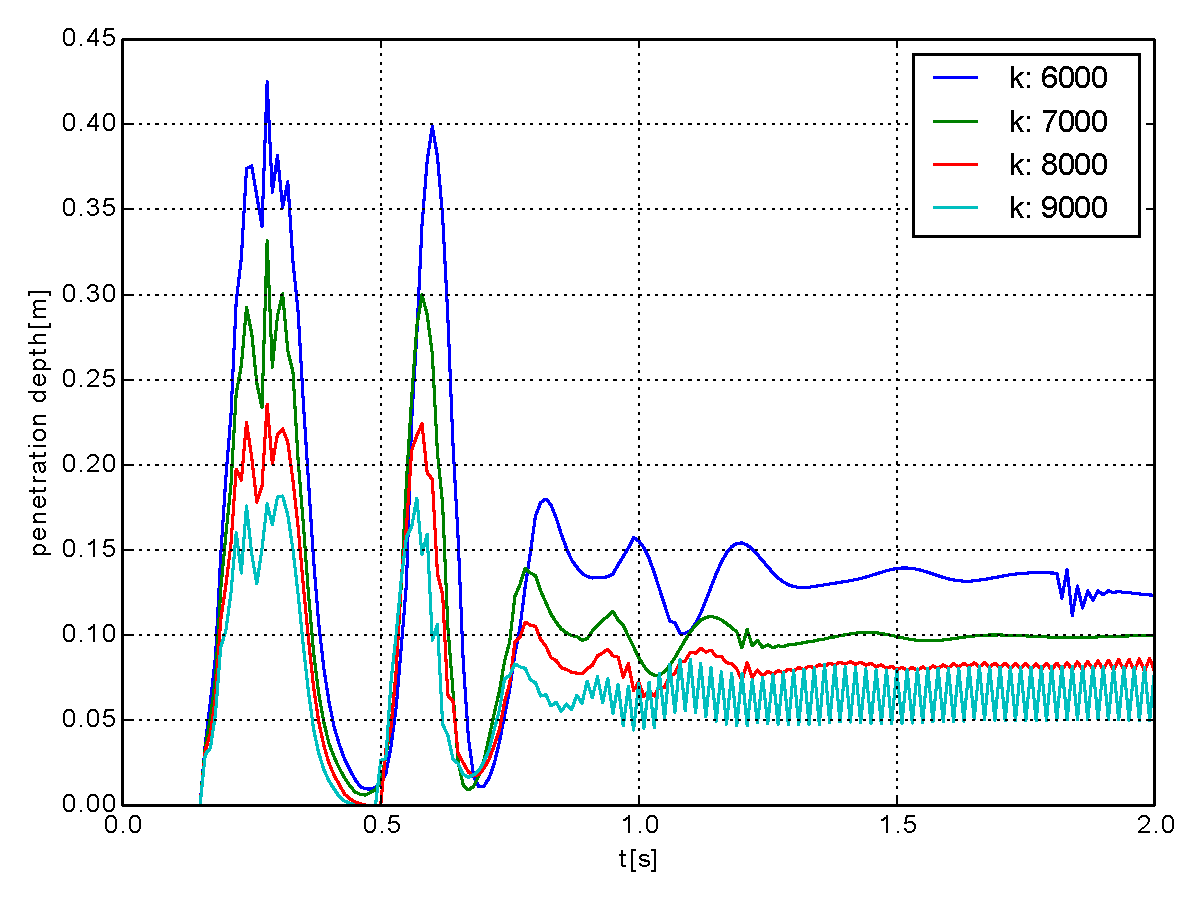
\includegraphics[width=0.9\textwidth]{pics/pdf/pre_corr.pdf}
  \caption[Predictor-Corrector scheme]{Illustration of the predictor-corrector scheme showing a particle colliding with a plane. 1) Prediction of the new velocity  2) Check for collisions along the new trajectory
  3) Applying correction impulses yields the final velocity
  4) Position update}
  \label{fig:pre_corr}
\end{figure}

In contrast to Bridson we do not check for proximity  since we do not differ between collision and contact and apply friction together with the repulsion impulses. So the integration scheme can be expressed as
\begin{enumerate}
\item
Advance simulation by one time step $\Delta t$ and set: $t^{n+1}=t^{n}+\Delta t$
\item
Predict new candidate velocities $\mathbf v^{n+1}_p$ according to external forces and bodies' interior dynamics 
\item Check linear trajectories for collisions between $t^n $ and $t^{n+1}$ using the position from the previous step $\mathbf x^n$ and $\mathbf v^{n+1}_p$
\item Repeat until no new collisions appear, maximum 5 iterations
	\begin{enumerate}[label*=\arabic*.]
	\item Compute repulsion and friction impulses for unhandled collisions
	\item Update $\mathbf v^{n+1}_p$ with the repulsion and friction impulses
	\item Check linear trajectories for collisions between $t^n $ and $t^{n+1}$ using the position from the previous step $\mathbf x^n$ and $\mathbf v^{n+1}_p$
	\end{enumerate}
	
\item Update velocity $\mathbf v^{n+1}=\mathbf v^{n+1}_p$
\item Update positions $\mathbf x^{n+1}=\mathbf x^n+ \Delta t \mathbf v^{n+1}$
\item Check for collision resolution and for redefinition
\item Rendering
\end{enumerate}
% Sunil Hadap, Dave Eberle, Pascal Volino, Ming C. Lin,
%Stephane Redon, and Christer Ericson. Collision detection and
%proximity queries proposed handling in chronological order

\chapter{Collision Detection}
\label{ch:CollisionDetection}
To provide a plausible accurate collision handling, it is essential to determine all colliding elements. Information about occurring collisions are provided by a collision detection algorithm.

We will present two different algorithms for computing intersections between triangle meshes. We first introduce a discrete collision test which tests for collisions at one moment in the time step. Afterwards, we extend the algorithm to a continuous formulation, by taking the feature trajectories into account. Thereby, we do not miss any collisions and additionally provide the contact times which are required for the CPF algorithm. Finally, we have a look at how the collision detection can be sped up with bounding volume hierarchies.

\section{Broad and Narrow Phase}
To check two bodies for intersections with elementary collision tests requires to test each element of the first body against all elements of the second body. Therefore, it scales in $O(nm)$ with $n$ and $m$ corresponding to the numbers of the surface vertices of the objects.
Since the amount of necessary tests is huge and performing all of them is expensive, most collision detections are divided into two stages.
The first stage, called "Broad Phase", uses a fast method to narrow the possibly colliding feature pairs down.
The second stage, called "Narrow Phase" applies an elemental test only to the remaining feature pairs.
The division in these two steps provides a significant speed-up \cite{BENDER2007}. In this thesis only a narrow phase is used.
\section{Discrete Collision Detection}
\label{sec:DCD}
An elementary discrete collision detection (DCD) test is to test for triangle-triangle collisions \cite{MOLLER1997}, which can be reduced to edge-triangle tests (based on \cite{Akenine-Moller2002}). All triangles of a body $A$ are tested against the edges of a body $B$ and vice versa. For a triangle $T$ with the vertices $\mathbf a$, $\mathbf b$ and $\mathbf c$, the plane $t$ defined by the triangle $T$ can be expressed as
\begin{equation}
t(\omega_b,\omega_c)=(1-\omega_b-\omega_c)\mathbf a +\omega_b \mathbf b + \omega_c \mathbf c,
\end{equation}
with the parameters $\omega_b$ and $\omega_c$ corresponding to the barycentric coordinates.

For an edge $E$ with the vertices $\mathbf p$ and $\mathbf q$ the line $e$ defined by the edge $E$ is
\begin{equation}
e(\omega_q)=\mathbf{p}+\omega_q (\mathbf{q}-\mathbf{p}),
\end{equation}
with the parameter $\omega_q$ corresponding to the barycentric coordinate.
The edge $E$ and the triangle $T$ collide if and only if $\exists \omega_q,\omega_b,\omega_c \in [0,1] \text{ such that}$
\begin{gather}
\label{eq::dcd-tv}
\mathbf{p}+\omega_q(\mathbf{q}-\mathbf{p})=(1-\omega_b-\omega_c)\mathbf a +\omega_b \mathbf b + \omega_c \mathbf c.
\end{gather}
If there exists a solution to the linear system \ref{eq::dcd-tv}, the plane and the line intersect. To ensure that the intersection is in the edge interval of the line, $ \omega_q$, $\omega_b$ and $ \omega_c$ need to be in the interval $[0,1]$.

To solve equation \ref{eq::dcd-tv} we transform it into a matrix formulation
\begin{equation}
	\mathbf{p}-\mathbf{a}=\begin{pmatrix}
	\mathbf{p}-\mathbf{q} \
	\mathbf b -\mathbf a \
	\mathbf c -\mathbf a
	\end{pmatrix}
	\begin{pmatrix}\omega_q\\\omega_b\\\omega_c
	\end{pmatrix}
\end{equation}
which can be solved using Cramer's rule.

\section{Continuous Collision Detection}
\label{sec:CCD}
Continuous collision detection (CCD) algorithms do not only detect whether two features are colliding but also when they are colliding, which is a property required by the CPF algorithm.
 Most CCD algorithms approximate the motion linearly, as described by Provot \cite{PROVOT1997}, but higher order formulations are also possible and provide a more accurate estimation of the collision times.
 
 For triangle meshes there are only two possible elementary collisions. Either a vertex goes through a triangle face resulting in a vertex-face (VF) collision or an edge goes through another edge resulting in an edge-edge (EE) collision, as shown in figure \ref{fig::asd}.

 
 We now describe how to compute collisions for both cases.
\begin{figure}[h!] 
\begin{minipage}[b]{0.5 \linewidth}
		\centering
		\subfigure[Vertex-face case]{
			       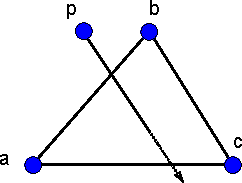
\includegraphics[width=0.5\linewidth]{pics/pdf/ccd_vf.pdf} }
	\end{minipage}
	\begin{minipage}[b]{0.5 \linewidth}
		\centering
		\subfigure[Edge-edge case]{
			       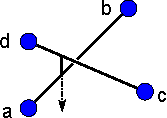
\includegraphics[width=0.5\linewidth]{pics/pdf/ccd_ee.pdf} }
	\end{minipage}

  \caption{Illustration of the possible feature pairs, VF and EE, for CCD.}
  \label{fig::asd}
\end{figure}

\paragraph{Vertex-Face}
For a moving vertex $\mathbf p(t)$ and a moving triangle $T$ with the vertices $\mathbf a(t)$, $\mathbf b(t)$ and $\mathbf c(t)$ the constant velocities associated to the linear motion are denoted as $\mathbf v_p$, $\mathbf v_a$, $\mathbf v_b$ and $\mathbf v_c$. For $t$ in the interval $[t_0,t_0+\Delta t]$, the vertex trajectories are $\mathbf p(t)=\mathbf p_0+t\mathbf v_p$, $\mathbf a(t)=\mathbf a_0+t\mathbf v_a$, $\mathbf b(t)=\mathbf b_0+t\mathbf v_b$ and  $\mathbf c(t)=\mathbf c_0+t\mathbf v_c$. The plane $f(t)$ defined by the triangle $T$ at the time $t$ can be expressed as
\begin{equation}
f(\omega_b,\omega_c,t)=(1-\omega_b-\omega_c)\mathbf a(t) +\omega_b \mathbf b(t) + \omega_c \mathbf c(t).
\end{equation}
The vertex $\mathbf p(t)$ and the triangle $T$ collide, if at one point in the time step $\mathbf p(t)$  is within $T$, which holds if and only if $\exists t \in [t_0,t_0+\Delta t], \; \exists \; \omega_b, \omega_c \in [0,1], \; \omega_b+\omega_c\le1 \text{ such that}$
\begin{gather}
\label{eq::ccd-vf}
\mathbf p_0+t\mathbf v_p=(1-\omega_b-\omega_c)\mathbf a(t) +\omega_b \mathbf b(t) + \omega_c \mathbf c(t).
\end{gather}
In contrast to the DCD the resulting equation system is non linear due to the new time dependency.
Therefore, we introduce the additional condition that at the time of collision, the vertex $\mathbf p(t)$ is coplanar to the triangle $T$. The additional condition is satisfied if $\mathbf{p}(t)-\mathbf{a}(t)$ is perpendicular to the triangle normal $\mathbf{n}_t(t)=(\mathbf{b}(t)-\mathbf{a}(t))\times(\mathbf{c}(t)-\mathbf{a}(t))$ giving
\begin{equation}
(\mathbf{p}(t)-\mathbf{a}(t)) \cdot \mathbf{n}_t(t)= \mathbf 0.
\end{equation}
This equation gives a third order polynomial with up to three real solutions $t_i$.
Any real $t_i$ in the interval $[t_0,t_0+\Delta t]$ will be inserted into condition \ref{eq::ccd-vf}, yielding a system of linear equations. Any $t_i$ 
satisfying both conditions is considered as a moment of collision.

\paragraph{Edge-Edge}
For a two moving edges $E_{ab}$ and $E_{cd}$ with the corresponding vertices $\mathbf a(t)$, $\mathbf b(t)$, $\mathbf c(t)$ and $\mathbf d(t)$ the constant velocities are $\mathbf v_a$, $\mathbf v_b$ $\mathbf v_c$ and $\mathbf v_d$. For $t$ in the interval $[t_0,t_0+\Delta t]$ the vertex trajectories are $\mathbf a(t)=\mathbf a_0+t\mathbf v_a$, $\mathbf b(t)=\mathbf b_0+t\mathbf v_b$, $\mathbf c(t)=\mathbf c_0+t\mathbf v_c$ and $\mathbf d(t)=\mathbf d_0+t\mathbf v_d$. The lines $e_{ab}(t)$ and $e_{cd}(t)$ defined by $E_{ab}$ and $E_{cd}$ can be expressed as 
\begin{gather}
e_{ab}(\omega_b,t)=\mathbf a(t)+ \omega_b(\mathbf b(t)-\mathbf a(t))\\
e_{cd}(\omega_d,t)=\mathbf c(t)+ \omega_d(\mathbf d(t)-\mathbf c(t))
\end{gather}
with the barycentric weights $\omega_b$ and $\omega_d$.\\ 
 Edge $E_{ab}(t)$ and edge $E_{cd}(t)$ collide if and only if $\exists t \in [t_0,t_0+\Delta t], \; \exists  \; \omega_b, \omega_d \in [0,1] \text{ such that}$
\begin{gather}
\label{eq::ccd-ee}
\mathbf a(t)+ \omega_b(\mathbf b(t)-\mathbf a(t))=\mathbf c(t)+ \omega_d(\mathbf d(t)-\mathbf c(t))
\end{gather}
Again this gives a non linear system and a further equation is necessary. At the time of collision, both edges are coplanar, which is fulfilled if the cross product of the edge vectors is perpendicular to an arbitrary vector from $E_{ab}$ to $E_{ac}$, which can be written
\begin{equation}
((\mathbf{b}(t)-\mathbf{a}(t))\times(\mathbf d(t) -\mathbf c(t)))\cdot(\mathbf c(t)- \mathbf a(t))=\mathbf 0
\end{equation}
Again this equation gives a third order polynomial with up to three solutions $t_i$.
Any $t_i$ in the interval $[t_0,t_0+\Delta t]$ will be inserted into condition \ref{eq::ccd-ee}, yielding a system of linear equations. Any $t_i$ 
satisfying both conditions is considered as a moment of collision.
\section{CCD Acceleration with Axis Aligned Bounding Boxes}
The elementary collision tests for CCD require more than 300 floating point operations per feature pair \cite{HUTTER2007}. 
%Due to the reason that generally only few elements collide in comparison to the number of elementary tests, we use a fas... 
In order to speed up the CCD, we apply axis aligned bounding boxes (AABB), since they provide a small computational overhead and narrow the necessary elementary tests. For CCD AABB span cuboids around the object primitives' trajectories, with the cuboid edges aligned to the coordinate axes \cite{PROVOT1997}, see figure \ref{fig:ccd_aabb}.
\begin{figure}[h] 
  \centering
     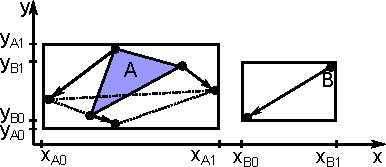
\includegraphics[width=0.7\textwidth]{pics/pdf/ccd_aabb.pdf}
  \caption[2D Illustration of  AABB to accelerate CCD by example of a triangle and a vertex.]{2D Illustration of  AABB to accelerate CCD by example of a triangle and a vertex. The arrows indicate the trajectory of the vertices within the time step. The boxes surrounding the features are the according AABB. The minimum and maximum coordinates for both AABB are consecutive in the x-direction. Therefore, there is no intersection.}
  \label{fig:ccd_aabb}
\end{figure}
To test for intersections between two AABB, the minimum and maximum values for each axis are sorted in ascending order. As long as for at least one axis the minimum and maximum coordinates for both AABB are consecutive there is no intersection. Otherwise, the AABB intersect and the elementary test needs to be applied.

We do not apply a hierarchical order of the AABB, as it is common used for bounding volume hierarchies \cite{TESCHNER2005}.


\chapter{Collision Handling with Penalty Methods}
\label{ch:DiscretePenaltyForces}
This chapter describes the collision handling with penalty methods.
We will first introduce the DPF and then extend the algorithm to a continuous formulation the CPF, taking the whole feature trajectory into account and thereby increasing stability and reducing jitter.
Afterwards, we present the penalty-based friction formulation.

Penalty methods handle constraints in a multi body system by applying forces opposed to the constraint violation to correct the velocity and position of the object. The strength of the force depends on the severeness of the constraint violation \cite{BENDER2007} and can be compared to a spring taking effect until the constraint is complied.

\section{Discrete Penalty Forces}
\label{sec:DiscretePF}
 The method of DPF defines a force field based on the penetration depth of two intersecting bodies. There are multiple definitions for penetration depth and the force field computation, we use the formulation presented by Tang et al. \cite{TANG2012}. For a point $\mathbf{x}$, belonging to object A and intersecting object B, the penetration depth $\delta(\mathbf{x})$ is defined as the distance to the closest point on the surface of B. Based on the penetration depth and the penalty coefficient $k$, the penalty energy is defined by
\begin{equation}
      E(\mathbf{x}) = \frac{1}{2}k \delta (\mathbf{x})^2 .
      \label{eq:penalty_energy}
\end{equation}
The formulation is similar to the energy $E_s(\mathbf x)$ of a spring system \cite{GROSS2011} %[p.224]
\begin{equation}
      E_{s}(\mathbf{x}) = \frac{1}{2} c ~||\mathbf{x-x_0}|| ^2,
\end{equation}
with the initial position $\mathbf x_0$ and the spring stiffness $c$.
The penalty coefficient $k$ corresponds to the spring stiffness $c$ and the penetration depth $\delta(\mathbf{x})$ corresponds to the spring expansion $||\mathbf{x-x_0}||$.
The penalty coefficient $k$ needs to be chosen in an empirical manner. According  its analogy to the spring stiffness, a similar behaviour can be observed. High penalty coefficients provide large contact forces and small intersections, however they also lead to unstable systems. On the other hand low penalty coefficients provide more stable systems with smaller forces but larger intersections. There is no exact rule how to choose the penalty coefficient, although we will show later (see section \ref{sec::stability}) that the relation $\Delta t \sim \sqrt{\frac{m}{k}}$ can be used as a rule of thumb.

According to the mechanical law of energy conservation \cite{WEBER2012} %[p.42]
 the  negative gradient of the penalty energy is the penalty force
\begin{equation}
      F(\mathbf{x}) = - \nabla  E(\mathbf{x})= - k \delta (\mathbf{x}) \nabla\delta (\mathbf{x}).
\end{equation}
With the definition of the penetration depth given above, the negative gradient of the penetration depth is equal to the unit surface normal $\mathbf{n}$ at the closest point on the surface of the penetrated object. The penalty force results in 
\begin{equation}
      F(\mathbf{x}) = k \delta (\mathbf{x}) \mathbf{n} 
            \label{eq:discrete_penalty_force}
\end{equation}
The impulse caused by DPF during a time step $\Delta t$ is the integral along time according to Newton's second law of motion
\begin{equation}
      I = \int_{t_i}^{t_i+\Delta t} F(\mathbf{x})dt=\Delta t F(\mathbf{x})=\Delta t k \delta (\mathbf{x}) \mathbf{n}. 
\end{equation}

The impulse can be applied to the vertices as described in section \ref{sec:InteractingRigDef}.

% !TeX spellcheck = en_GB
\section{Continuous Penalty Forces}
\label{sec:ContinuousPenaltyForces}
This section outlines the algorithm CPF presented by Tang et al. \cite{TANG2012}, which reduces instability and jitter in comparison to DPF and is the basis for this thesis. The general impulse formula for the vertex-face and edge-edge case will be derived and the exact formula for the case of linear interpolated trajectories will be presented.

\subsection{CCD and Penetration Depth}
\label{sec:CCDandPenetrationDepth}
To simplify the collision response with CPF, each simulation time step is normalized to the unit interval $[0, 1]$. The collisions are detected using a CCD algorithm, as described in section \ref{sec:CCD}, considering all possible pairwise features, VF and EE. Furthermore, the CCD provides the contact times for each feature pair and the collision points $\mathbf p(t)$ and $\mathbf q(t)$ at the first time-of-contact. The points $\mathbf p(t)$ and $\mathbf q(t)$ are traced along their trajectories until the collision is resolved.

In contrast to DPF, the penetration depth is defined by a formulation utilizing the information provided by CCD. A contact normal is defined for each contact pair. In the VF case, the time-dependent contact normal $\mathbf n(t)$ is the normal of the colliding triangle. In the EE case, the time-dependent contact normal $\mathbf n(t)$ is the cross product of the two edge vectors. The penetration depth is defined as the vector between the two contact points $\mathbf p(t)$ and $\mathbf q(t)$ projected onto the contact normal
\begin{equation}
       	\delta(t)  =\mathbf{n}(t) \cdot  (\mathbf p (t) - \mathbf q (t))
\end{equation}
A feature pair is considered colliding, from the first time of contact until the penetration depth is strictly positive. Within a normalized simulation time step the penetration time interval $[t^i_a , t^i_b] \in [0,1]$ is the interval in which the feature pair is colliding.
With linear trajectories, up to two penetration time intervals can occur within one time step, since the elementary collision test can return up to three real roots. For higher-degree trajectories even more time intervals can occur.

\subsection{Continuous Penalty Forces}
\label{sec:CPFGENERAL}
The CPF approach extends the idea of DPF and computes collision impulses by continuously accumulating penalty forces along the penetration depth over the whole time step. Thereby, not only the position at one moment but also the trajectory is included in the computation of the impulse.

The CPF $\mathbf F (t)$ is computed analogously to the DPF, but now with time-dependent definitions for the normal $\mathbf n (t)$, penetration depth $\mathbf{\delta}(t)$
\begin{equation}
    \mathbf  F(t) = k \delta (t) \mathbf{n} (t) = k\mathbf{n}(t) \cdot  (\mathbf p(t) - \mathbf q (t)) \mathbf{n} (t).
\end{equation}
The resulting impulse is computed with regard to the penetration intervals
\begin{equation}
\label{eq::CPF_impulse}
     \mathbf I = \int_{t_i}^{t_i+\Delta t} \mathbf F(t)dt= \sum\limits_{i=0}^{n}\int_{t_a^i}^{t_b^i}\mathbf F(t)dt=k \sum\limits_{i=0}^{n}\int_{t_a^i}^{t_b^i} \mathbf{n}(t) \cdot   (\mathbf p(t) - \mathbf q (t)) \mathbf{n} (t)dt.
\end{equation}
An illustration of the impulse computation is provided in figure \ref{fig:impulseComputationCPFDPF}. The linear trajectory can be approximated exactly by the CPF, see figure \ref{fig:impulseComputationCPFDPF} a) and c). Whereas, the DPF overestimate the penetration depth as long as the penetration depth is increasing, see figure \ref{fig:impulseComputationCPFDPF} b). The DPF underestimated the penetration depth as long as it is decreasing, see figure \ref{fig:impulseComputationCPFDPF} d).

\begin{figure}[h] 
  \centering
     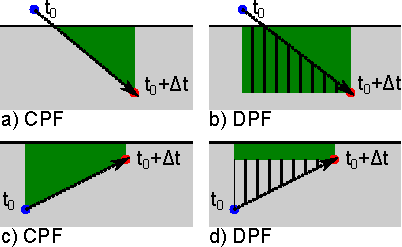
\includegraphics[width=0.7\textwidth]{pics/pdf/impulseComputationCPFDPF.pdf}
  \caption[2D Illustration of the resolution force computation for CPF and DPF in the VF case.]{2D Illustration of the resolution force computation for CPF and DPF in the VF case. The blue dot marks the position of the vertex of object A at the beginning of the time step and the red dot the predicted end position. The dotted arrow indicates the linearly approximated trajectory. The grey area is the inside of object B. The green area corresponds to the integral over the force and thereby the resolution impulse. The black striped areas indicate the estimation errors of the DPF forces. It is noticeable that the DPF overestimates the penetration depth as long as the penetration depth is increasing, see subfigure b), and underestimates the penetration depth as long as it is decreasing, see subfigure d).}
  \label{fig:impulseComputationCPFDPF}
\end{figure}

 
\subsection{Vertex-Face Contact Forces}
In the VF case, the contact point $\mathbf p(t)$ is the position of the colliding vertex V and  the contact point $\mathbf q(t)=\omega_a \mathbf a(t)+\omega_b \mathbf b(t)+\omega_c \mathbf c(t) $ is the representation of the collision point on the triangle T in barycentric coordinates with the vertex positions $\mathbf a$, $\mathbf b$ and $\mathbf c$ and their corresponding weights $\omega_a$, $\omega_b$ and $\omega_c$. The contact normal $\mathbf n_T(t) = (\mathbf b(t) - \mathbf a(t))\times(\mathbf c(t) - \mathbf a(t))$ is the normal of the triangle. With equation \ref{eq::CPF_impulse}, the impulse on the vertex p is
\begin{equation}
     \mathbf I_p =k \sum\limits_{i=0}^{n}\int_{t_a^i}^{t_b^i} \mathbf{n_T}(t) \cdot   (\mathbf p(t) - \omega_a \mathbf a(t)-\omega_b \mathbf b(t)-\omega_c \mathbf c(t)) \mathbf {n_T} (t)dt.
\end{equation}
The impulse on the triangle is distributed among the three vertices according to the barycentric weights

\begin{equation}
     \mathbf I_a =- \omega_a \mathbf I_p, 
     \mathbf I_b =- \omega_b \mathbf I_p,
     \mathbf I_c =- \omega_c \mathbf I_p.
\end{equation}
For linear interpolated motions, the velocity is constant and can be computed with the vertices' start and end position $\mathbf (\mathbf p_0,\mathbf p_1)$, $(\mathbf a_0,\mathbf a_1)$, $(\mathbf b_0,\mathbf b_1)$ and $(\mathbf c_0,\mathbf c_1)$ as $\mathbf v_p=\mathbf p_1-\mathbf p_0$ and similarly for $\mathbf v_a$, $\mathbf v_b$ and $\mathbf v_c$.
With the second order Bernstein polynomials
\begin{equation}
B^2_i(t)=\frac{2!}{i!(2-i)!}t^i(1-t)^{2-i}
\end{equation}
and the constant basis coefficients $\mathbf n_0=(\mathbf b_0- \mathbf a_0) \times (\mathbf c_0-\mathbf a_0)$, $\mathbf n_1= \frac{\mathbf n_0+ \mathbf n_2 - (\mathbf v_b-\mathbf v_a) \times (\mathbf v_c - \mathbf v_a)}{2}$ and $\mathbf n_2=(\mathbf b_1- \mathbf a_1) \times (\mathbf c_1-\mathbf a_1)$ and the normalization factor $L(t)$, the time varying contact normal is
\begin{equation}
	\mathbf{n_T}(t)=\frac{\mathbf{n_0}B^2_0(t)+\mathbf{n_1}B^2_1(t)+\mathbf{n_2}B^2_2(t)}{L(t)}.
\end{equation}
The normalization factor $L(t)$ is composed as
\begin{equation}
	L(t)=\sqrt{(L_0L_1...L_4)(B^4_0(t)B^4_1(t)...B^4_4(t))},
\end{equation}
with the factors $L_i$, which are given in the supplementary material of \cite{TANG2012}.


To compute the impulse exactly, it would be necessary to integrate the rational function $n_T$ which is rather complicated because of the denominator $L(t)$ \cite{TANG2012}.
Tang et al. suggest to approximate $L(t)$ by a constant $L_k$
\begin{equation}
	L(t)\approx L_k=\sqrt{\frac{L_0+L_1+L_2+L_3+L_4}{5}}.
\end{equation}
With this approximation the normal is a quadratic term and the computation of the integral is simplified, resulting in speed-ups up to an order of magnitude without noticeable differences in the simulation results \cite{TANG2012}.

\subsection{Edge-Edge Contact Forces}
In the EE case, the contact points $\mathbf p(t)=\omega_a \mathbf a(t)+\omega_b \mathbf b(t)$ and $\mathbf q(t)=\omega_c \mathbf c(t)+\omega_d \mathbf d(t) $ are the barycentric representation of the collision points on the edges $E_1$ and $E_2$ with the vertex positions $\mathbf a(t)$, $\mathbf b(t)$, $\mathbf c(t)$ and $\mathbf d(t)$ and their corresponding weights $\omega_a$, $\omega_b$, $\omega_c$ and $\omega_d$.
The contact normal $\mathbf{ n_E}(t) = (\mathbf b(t) - \mathbf a(t))\times(\mathbf d(t) - \mathbf c(t))$ is the cross product of the two edge vectors.  With equation \ref{eq::CPF_impulse} the impulse on the edge $E_1$ is
\begin{equation}
     \mathbf I_E =k \sum\limits_{i=0}^{n}\int_{t_a^i}^{t_b^i} \mathbf{n_E}(t) \cdot   (\omega_a \mathbf a(t)+\omega_b \mathbf b(t)-\omega_c \mathbf c(t)-\omega_d \mathbf d(t)) \mathbf {n_E} (t)dt.
\end{equation}
The impulse is distributed among the four vertices according to the barycentric weights
\begin{equation}
     \mathbf I_a = \omega_a \mathbf I_E, 
     \mathbf I_b = \omega_b \mathbf I_E,
     \mathbf I_c =- \omega_c \mathbf I_E,
     \mathbf I_d =- \omega_d \mathbf I_E.
\end{equation}
Similar to the VF case, for linear interpolated motion the velocity is constant and the velocity can be computed from the vertices' start and end positions  $(\mathbf a_0,\mathbf a_1)$, $(\mathbf b_0,\mathbf b_1)$, $(\mathbf c_0,\mathbf c_1)$  and $(\mathbf d_0,\mathbf d_1)$ as $\mathbf v_a=\mathbf a_1-\mathbf a_0$ and analogously for $\mathbf v_b$, $\mathbf v_c$ and $\mathbf v_d$. With the second order Bernstein polynomials 
\begin{equation}
B^2_i(t)=\frac{2!}{i!(2-i)!}t^i(1-t)^{2-i}
\end{equation}
and the constant basis coefficients $\mathbf n'_0=(\mathbf b_0- \mathbf a_0) \times (\mathbf d_0-\mathbf c_0)$, $\mathbf n'_1= \frac{\mathbf n'_0+ \mathbf n'_2 - (\mathbf v_b-\mathbf v_a) \times (\mathbf v_d - \mathbf v_c)}{2}$ and $\mathbf n'_2=(\mathbf b_1- \mathbf a_1) \times (\mathbf d_1-\mathbf c_1)$ and the normalization factor $L(t)$, the time varying contact normal can be expressed as

\begin{equation}
	\mathbf{n_T}(t)=\frac{\mathbf n'_0 B^2_0(t)+\mathbf n'_1 B^2_1(t)+\mathbf n'_2 B^2_2(t)}{L(t)}
\end{equation}
The normalization factor $L(t)$ can be computed as in the VF case.


We now give an example how to apply CPF for collisions for a static ground plane.
Ground collisions are a common scenario in many environments and due to the static plane the formula can be simplified.

 For collisions with the ground plane in an environment with gravity in the negative y-direction, the contact normal $\mathbf{n_P}=(0,1,0)$ is constant. With the position of the colliding vertex $\mathbf p(t)$ the impulse is

\begin{equation}
     \mathbf I_p =k \sum\limits_{i=0}^{n}\int_{t_a^i}^{t_b^i} \mathbf{n_P} \cdot   \mathbf p(t) \mathbf {n_P}dt=k \sum\limits_{i=0}^{n}\int_{t_a^i}^{t_b^i} (0,p_y(t),0)  dt,
\end{equation}
with $p_y(t)$ the $\mathbf p(t)$ component in $y$-direction.

Again we assume linear interpolated motion for the particle $\mathbf p(t)= \mathbf{p_0}+t \mathbf{v_p}$. Solving the integral gives a quadratic expression for the vertex impulse
\begin{equation}
 \mathbf I_p=(0,(t_a-t_b) kp_y(t_0)-\frac{t_b^2-t_a^2}{2} kv_y,0).
\end{equation}
No outer sum is required, since maximum one penetration interval can occur.
%Since we only detect and handle vertex-ground collisions, it is necessary to compensate the potential edge-ground forces by the vertex-ground for to reach a consistent contact handling in the scene. Otherwise the body-body collisions are stiffer than the body-ground collisions. The ratio of vertices to edges, was for multiple tested meshes $1:2.98 \pm 0.03$, see appendix \ref{TODO}, giving us a compensation factor of $1+2.98\approx4$. For ground collisions we compute the impulse with a modified stiffness coefficient $k^*=4k$ resulting in an new impulse
%\begin{equation}
%     \mathbf I_p^* =k^* \sum\limits_{i=0}^{n}\int_{t_a^i}^{t_b^i} (0,p_y(t),0)\cdot dt
%\end{equation}

\section{Friction}
\label{ch:Friction}
We model friction with a penalty-based model by Yamane and Nakamura\cite{YAMANE2006}, providing a straightforward integration in the penalty based collision resolution, only small computational overhead and an unified handling for rigid and deformable bodies. The penalty-based formulation differs between dynamic and static friction, similar to  Coulomb's friction law. 
Coulomb's friction law \cite{YAMANE2006} defines the friction force $\mathbf f_f$ as
\begin{equation}
\mathbf f_f=
\begin{cases}
\mathbf f_s & \text{ if } |v_{slip}|=0 \text{ and } |\mathbf f_{s}|\le\mu_S |\mathbf f_n| \\
\mu_D \mathbf f_n & \text{ else }
\end{cases}
\end{equation}
with the static and dynamic friction coefficients $\mu_s$ and $\mu_d$ and the normal force $\mathbf f_n$.
For the model by Yamane and Nakamura, we first compute the static friction force $\mathbf f_s$ as
\begin{equation}
\mathbf f_s= (k_{FP}(\mathbf p_{ref} - \mathbf p)-k_{FD}\mathbf v_{slip} )
\end{equation}
with the penalty coefficients $k_{FP}$ and $k_{FD}$, the current position $\mathbf p$ and the reference position $\mathbf p_{ref}$, where $\mathbf p$ is to be fixed. $\mathbf p_{ref}$ is initialized when the features come into contact with the contact point and is updated to the current position $\mathbf p$ each time dynamic friction is applied. Similar to Coulombs law, we apply static friction, if $|\mathbf f_s|\le\mu_s|\mathbf f_n|$. Otherwise we apply dynamic friction as
\begin{equation}
\mathbf f_d=-\mu_d |\mathbf f_n| \frac{\omega (|\mathbf{v}_{slip}|)}{|\mathbf{v}_{slip}|}\mathbf{v}_{slip},
\end{equation}\\
with the continuous weighting function $\omega(x)$.  $\omega(x)$ is defined by
\begin{equation}
\omega(x)=1-e^{-k_\omega x}
\end{equation}
with the positive constant $k_\omega$. $\omega (x)$ satisfies $\omega(0)=0$ and $\lim_{x \rightarrow + \infty}\omega(x)=1$. Furthermore, $\omega(x)$ solves the potential singularity arising from the division by $|\mathbf v_{slip}|$ for small $|\mathbf{v}_{slip}|$, since 
\begin{equation}
\lim\limits_{x\rightarrow 0}\frac{\omega (x)}{x}=k_{\omega}.
\end{equation}
Therby, for $|v_{slip}| \ll 1$ the dynamic friction can be approximated as
\begin{equation}
\mathbf f_d=-\mu_d |\mathbf f_n| k_{\omega}\mathbf{v}_{slip}.
\end{equation}


The static friction model is similar to applying a damped spring at the contact point. If the spring force is too large, dynamic friction is applied.
\include{continuous_penalty}
\chapter{Robust handling of enduring contacts}
\label{ch:RobustHandlingofSlidingContacts}
This chapter outlines the artifacts we observed emerging from the CPF algorithm \cite{TANG2012} and our approaches to treat them. We will first give a brief overview on the artifacts and then describe them in detail. Subsequently, we will describe our approaches to handle the artifacts.

\section{CPF Artifacts}
\label{sec::CPFArtifacts}
The CPF collision handling as described by Tang et al. \cite{TANG2012} shows artifacts, in particular for enduring contacts. Enduring contacts are contacts, which are not resolved in the time step they occur. We observed three major artifacts, separated features still assumed colliding, additional artificial collisions through discretization and inconsistent feature pair mapping. The artifacts emerge if collisions from previous time steps are not completely resolved and additionally a colliding features performs a motion tangential to the surface it is intersecting. In particular, such a behavior can be observed for sliding and deep collisions.

\subsection{Separated Features Still Assumed Colliding}
\label{ss:ResolvedCollisionsRemain}

\begin{figure}[h!] 
  \centering
     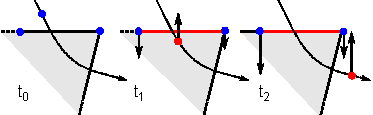
\includegraphics[width=0.75\textwidth]{pics/pdf/slidingVertexArtifactUnresolvedCollision.pdf}
  \caption[2D-Illustration of a VF collision, which is considered colliding after it is already resolved]{2D-Illustration of a VF collision, which is considered colliding after it is already resolved. Dots indicate the vertices, the red ones are colliding. The straight lines indicate the the surface triangles, the red ones are colliding. The black arrows indicating the applied impulses.  $t_0$ no collision; $t_1$ the single vertex is colliding with the red triangle; $t_2$ the single vertex is still colliding with the red triangle, although it left the body through the black face.}
  \label{fig:slidingVertexArtifactUnresolvedCollision}
\end{figure}

A feature pair is considered colliding as long as the penetration depth is strictly negative \cite{TANG2012}.
This can lead to feature pairs, which are considered colliding even 
if the bodies are already separated.
The collision resolution is missed if a feature is colliding with another feature and leaves the body by passing through a third feature, without reducing the original penetration depth to zero. A good example for such a scenario is shown in figure \ref{fig:slidingVertexArtifactUnresolvedCollision}. A vertex enters a cube through the top face and leaves the cube through a side face, however the separated features are still assumed to be colliding.

For EE collisions a similar behavior can be observed. For EE collisions it is additionally possible that an edge leaves the body without colliding with another edge.



\subsection{Additional Artificial Collisions Through Discretization}
\label{ss:DiscretizationCollisonForces}

Consider a cube colliding with an analytical static plane. Correctly there are only impulses applied to the object in the direction normal to the plane and the cube's tangential velocity does not change.
If we swap the analytical plane for a discretized triangle surface mesh, again we would expect that only impulses are applied which show in the direction normal to the plane. 
However, collisions arise with normals showing in a direction tangential to the plane. They stop the tangential movement directly and and hook the body in the surface, as shown in figure \ref{fig:slidingVertexArtifactDiscretizationForces}. These collisions arise between the edges and vertices of the plane with the edges and faces of the cube. However, the edges and vertices of the plane are only a product of the discretization and should not induce tangential forces.

The artifact can be described more generic as follows. When two bodies collide with non-zero tangential velocity or with deep intersections, collisions arise with contact normals showing in a direction tangential to the surfaces. This makes the objects collide sidewards, stops the tangential movement and hooks the objects between surface elements.

In our simulations the consequences of this artifact were severe to such an extent that a simulation of collisions with even only small tangential movement was not possible.
\begin{figure}[h] 
  \centering
     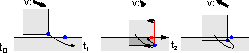
\includegraphics[width=0.95\textwidth]{pics/pdf/slidingVertexArtifactDiscretizationForces.pdf}
  \caption[2D-Illustration of a hooked VF collision with tangential forces induced by the CPF algorithm.]{2D-Illustration of a hooked VF collision with tangential forces induced by the CPF algorithm. For the sake of clarity, only the artifact collision is highlighted.  $t_0$ no collision; $t_1$ the red face collides with the surface vertex of the lower body resulting in forces almost tangential to the surface of the lower body and reverting the tangential movement; $t_2$ the artifact collision is resolved, however the colliding object completely reverted its velocity, similar to a collision with a artificial wall.}
  \label{fig:slidingVertexArtifactDiscretizationForces}
  

\end{figure}


\subsection{Inconsistent Feature Pair Mapping}
\label{ss:ImplausibleFeaturePairs}
When two features collide, the feature pair and the barycentric weights are stored for further collision treatment and used until the collision is resolved \cite{TANG2012}.

 For the VF case, this can lead to implausible feature pairs when a vertex moves tangential to the surface of the body it is intersecting.
The implausible feature pairs arise if the vertex continues its tangential movement and moves below a neighboring triangle, as shown in Fig \ref{fig:slidingVertexArtifactImplausibleForces}. As a result there are large distances between the vertex and the colliding triangle, which results in impulses at distant vertex positions. This leads to implausible behavior as an object is deformed at positions distant from the collision.

\begin{figure}[h!] 
  \centering
     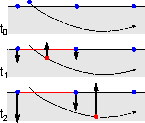
\includegraphics[width=0.4\textwidth]{pics/pdf/slidingVertexArtifactImplausibleForces.pdf}
  \caption[2D-Illustration of a VF collision causing impulses at implausible positions.]{2D-Illustration of a VF collision causing impulses at implausible positions.
  At time $t_0$ there is no collision. At time $t_1$ the single vertex is colliding with the red triangle. At time $t_2$ the single vertex is still colliding with the red triangle, although the vertex shifted under the triangle right to the red one.}
  \label{fig:slidingVertexArtifactImplausibleForces}
\end{figure}

In the case of EE collisions, a similar behavior can be observed. When an edge moves tangential to the surface of the body it is intersecting and the edge slides below another edge, impulses are applied at distant positions. 

Furthermore, the implausible feature pairs can lead to wrong resolutions of collisions, as shown in figure \ref{fig:slidingVertexSmallRotation}. With a large distance between the two colliding features, only a minor rotation of the colliding face or an colliding edge is necessary to reduce the penetration depth to zero. Thereby the resolution condition (given in section \ref{sec:CCDandPenetrationDepth}) is fulfilled, whereas the feature might still be intersecting the body.
\begin{figure}[h] 
  \centering
     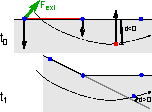
\includegraphics[width=0.4\textwidth]{pics/pdf/slidingVertexSmallRotation.pdf}
  \caption[2D-Illustration of an incorrect VF collision resolution artifact]{2D-Illustration of an incorrect VF collision resolution artifact. At time $t_0$ the single vertex is colliding with the red triangle and a external force is applied to the red triangle. At time $t_1$ the red triangle rotated, the distance of the vertex to the triangle plane is now positive and thereby the collision resolution condition is incorrectly satisfied.}
  \label{fig:slidingVertexSmallRotation}
\end{figure}
This unwanted resolution appears for example when a rigid cube is dropped on a deformable bar and afterwards the rigid cubes slides on the bar. Due to impact of the rigid body, the surface of the deformable body oscillates and the surface triangles perform small rotations. These rotations are sufficient to fulfill the resolution condition. Thereby the collision is "resolved", whereas the vertex should still be colliding since it is intersecting the body.


\section{CPF Extensions}
\label{sec::CPFExtensions}
To maintain plausible feature pairs and correct resolution impulses, extensions of the original CPF algorithm are necessary.
In total we introduce three additional steps solving and reducing the issues described in the previous section. % as described in detail in the following. %:
%To solve the resolved collisions remaining we introduce an advanced resolution condition.
%To handle the implausible feature pairs we introduce a redefinition algorithm.
%To prevent the discretization collision forces, we categorize the contacts in regular, sliding or hooked and treat the collisions accordingly.


\subsection{Advanced Resolution Condition}
\label{ss:AdvResCond}
To accomplish a correct resolution detection and to avoid the separated features still assumed colliding, we extend the resolution condition by additionally taking collisions of the features' vertices into account.

For the VF case, we consider a collision resolved, if either the penetration depth is positive or the colliding vertex collides with another face of the intersecting body. This condition is sufficient, since no collision is missed due to the CCD. Therefore, when the collision resolves the vertex passes the surface of the body it is intersecting and thereby a triangle vertex contact is detected. 

For the EE case we consider a collision resolved, if either the penetration depth is positive or when both vertices of an edge are resolved and the edge is not intersecting a face of the previously intersected body.
This condition is sufficient, since when the edge is colliding, but none of the edge's vertices is colliding, the edge pierces the surface and thereby the edge intersects a triangle. Otherwise, the edge is not colliding.

\subsection{Contact Categorization}
\label{ss::ContactCategorization}
As described in section \ref{ss:DiscretizationCollisonForces}, some collisions generate artifact forces when the tangential velocity is non-zero. To avoid the artifact forces we need to distinguish these collisions from the regular collisions. Therefore, we introduce conditions in order to categorize the collisions either as "regular", which can be handled with the regular algorithm or as "hooked", which generate artifact forces and require special handling. The categorization is limited to non-deep contacts, though we will discuss possibilities to extend the categorization to deep collisions at the end of the section.

A \textbf{regular} collision is considered as the common case, with the two bodies being pushed away from each other. This applies for collisions with the surface normals of the colliding features showing in opposite directions and the resolution impulses showing inside the according bodies. Regular collisions are handled with the original algorithm.

A \textbf{hooked} collision appears for sliding contacts or deep intersections. The surface normals are closer to an orthogonal state than to an opposing state. This results in impulses tangential to a surface. These collisions are implausible since the tangential motion should not change without friction. The body hooks in the surface, as it can be seen in figure \ref{fig:slidingVertexArtifactDiscretizationForces}.
Therefore, we redefine the feature pairs of hooked collisions in order to reduce the tangential impulses and to gain regular collisions.

In the following we will discuss the formulation with an emphasis on the VF case. Afterwards, we will give the definition for the EE case, which is analogous.

The previous description yields the basic formulation of the condition for a hooked collision:  A collision is hooked, if the proportion of the contact normal  $\mathbf{n_{c}}$ in a direction tangential to the surface of a feature is larger than the proportion in the direction normal to the surface. Otherwise, the collision is regular. The contact normal is equal to the direction of the applied collision impulse. To express the surface direction of a vertex, we apply the averaged vertex normal $\mathbf{n_{v}}$ as the average of the adjacent face normals and handle it as a surface normal. The condition for a hooked collision can now be expressed with the dot product as
\begin{equation}
-\mathbf{n_{v} \cdot n_{c}}<\cos(45^\circ)=\frac{\sqrt 2}{2},
\end{equation}
with a negative sign before the dot product since the two normals are opposing.
This relation is illustrated in the classification circle, see figure
\ref{fig::classification}. It is not necessary to additionally check the triangle normal against the contact normal since the contact normal is equal to the triangle normal. Thereby, they are per definition always showing in the same direction.
\begin{figure}[tbp] 
  \centering
     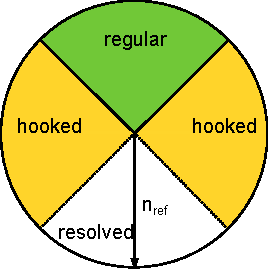
\includegraphics[width=0.4\textwidth]{pics/pdf/classification.pdf}
  \caption[2D-Illustration of the classification circle.]{The classification circle is an illustration of the condition for a hooked collision. Depending on the surface normal $n_v$, as shown as example by the grey arrow, and the fixed contact normal $\mathbf n_c$it is possible to determine whether a collision is hooked or regular.}
  \label{fig::classification}
\end{figure}
\begin{figure}[tbp] 
  \centering
     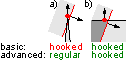
\includegraphics[width=0.55\textwidth]{pics/pdf/anglesOfAttack.pdf}
  \caption[Comparison of the contact categorization with normals and normal spans.]{Comparison of collisions of vertices in acute-angled and an obtuse-angled corners. The subfigures a) and b) have the same relation between the contact normals and the averaged vertex normal. Therefore, the basic formulation yields that both collisions are hooked. However, for a) the contact normal is almost parallel to the two face normals, therefore we would expect an regular collision.}
  \label{fig::anglesOfAttack}
\end{figure}

The basic formulation is insufficient for vertices in acute-angled corners, as shown in the following.
Vertices in acute-angled corners of a tetrahedron can collide in a larger area of contact angles than vertices in obtuse-angled corners, as shown in figure \ref{fig::anglesOfAttack}.  The figure compares collisions of vertices in acute-angled and an obtuse-angled corners. The subfigures a) and b) have the same relation between the contact normals and the averaged vertex normal. Therefore, the basic formulation yields that both collisions are hooked. However, for subfigure a) the contact normal is almost parallel to the two face normals, therefore we would expect a regular collision. Furthermore, the angle between the averaged vertex normal the normal of the adjacent faces is large, it is close to $90^\circ$. Thereby, the averaged vertex normal does not provide a sufficient expression of the surface normal for acute-angled corners.


Therefore, we need to introduce a construct taking the angles between adjacent face normals into account.
 Accordingly, we introduce a cone alike span $\mathbf{N}$ (see figure \ref{fig::vertexNormalSpan}) spanned by the surface normals of the directly adjacent faces of the vertex or edge. It will be called "normal span" in the following. 
\begin{figure}[h] 
  \centering
     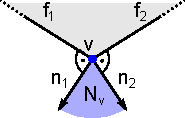
\includegraphics[width=0.4\textwidth]{pics/pdf/vertexNormalSpan.pdf}
  \caption[2D-Illustration of the vertex normal span $\mathbf{N_v}$ of the vertex v.]{2D-Illustration of the vertex normal span $\mathbf{N_v}$ of the vertex v. The normals of the faces $\mathbf{f_1}$ and $\mathbf{f_2}$ are indicated $\mathbf{n_1}$ and $\mathbf{n_2}$. The vertex normal span is indicated in light blue.}
  \label{fig::vertexNormalSpan}
\end{figure}
The normal span is large for acute-angled corners and small for obtuse-angled corners. Thereby, the normal span reflects the collision behavior for vertices in such corners and a proper contact categorization is possible (see figure 
\ref{fig::vertexNormalSpanComp}). The illustration compares the collision category evaluation for the collisions with averaged normals and normal spans. It emphasizes that with normal spans an accurate collision categorization can be provided, regardless of the angle in the vertex corner.
\begin{figure}[h] 
  \centering
     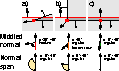
\includegraphics[width=0.65\textwidth]{pics/pdf/stupidNormals2.pdf}
  \caption[Comparison of the contact categorization with normals and normal spans for VF collisions with the vertex in an acute-angled, right-angled and obtuse-angled corner.]{Comparison of the contact categorization with normals and normal spans for VF collisions with the vertex in an acute-angled, right-angled and obtuse-angled corner. a) shows a acute-angled corner of a tetrahedron colliding with a flat surface. The normal span indicates correctly a regular collisions, in contrast to the normals indicating a hooked collision.  b) shows a  right-angled corner of a cube colliding with a flat surface. The normal span indicates correctly a regular collisions, for the normals it is exactly the border between hooked and valid.  c) shows a vertex of a flat surface colliding with a flat surface. Both, the normal span and the normals indicate the collision correctly as regular.}
  \label{fig::vertexNormalSpanComp}
\end{figure}

To implement the normal span in the simulation, we need to discretized it.
Therefore, we approximate the normal span by the set of triangle normals adjacent to the vertex or edge.
For edges only the two directly adjacent faces are considered. For the approximation of larger normal cones we additionally add the averaged vertex normal to the set.


For the contact categorization the normal cone is an often used element.
To avoid a large computation overhead due to searching of neighboring elements in order to compute their normal, it is necessary to apply a data structure providing fast neighborhood information. 
We use a data structure by Serna et al. \cite{SERNA2009B} providing the necessary fast neighborhood information.


The previously introduced category definitions are implemented as follows. 
A VF collision is hooked, if the proportion of the contact normal showing in the direction tangential to the vertex surface is larger than proportion showing in the normal direction, expressed similar to the basic formulation as
\begin{equation}
\min(\mathbf{\{n_{Vi} \cdot n_{cv}\}})>-\frac{\sqrt 2}{2} \; | \; \mathbf{n_{Vi}} \in \mathbf{N_{v}},
\end{equation} with the normal span of the vertex $\mathbf{N_{v}}$ and the contact normal $\mathbf{n_{cv}}$. This formulation is similar to measuring the minimum angle between the normal span and the negative contact normal. If this angle is larger than $45^\circ$ the impulse proportion tangential to the face is larger than normal proportion and the collision is hooked.
Otherwise the collision is regular.


A EE collision is hooked,  if the proportion of the contact normal showing in the direction tangential to the surface is larger than proportion showing in the normal direction for both edges, expressed similar to the basic formulation as
\begin{equation}
\min(\mathbf{\{{n}_{Eai}\cdot{n}_{ce}\}})>-\frac{\sqrt 2}{2} \; \land  \; \max(\mathbf{\{{n}_{Ebi}\cdot{n}_{ce}\}})<\frac{\sqrt 2}{2} \; | \;, \mathbf{n_{Eai}} \in \mathbf{N_{Ea}},\; \mathbf{n_{Ebi}} \in \mathbf{N_{Eb}}
\end{equation} with the normal spans $\mathbf{N}_{Ea}$ and $\mathbf{N}_{Eb}$ of the edges and the contact normal $\mathbf{n_{ce}}$.

If the collision is not hooked, it is regular.

The handling of regular collisions is straightforward. Regular collisions are handled with the CPF algorithm without modification. The handling on hooked contacts is based on the algorithm for the redefinition of feature pairs in the next section \ref{ss::redef}. Therefore, the handling of hooked contacts is described in section \ref{ss::sliding}.

In the beginning of this section we have stated that the categorization is only applicable for non-deep collisions. Now we will investigate the problem arising from deep collisions and how it could be solved.

This collision definition is limited to non-deep intersections, since we can not differentiate between a hooked contact and a deep intersection with only the local collision data, see figure \ref{fig::limitCategory}. On the left side the local collision arrangement is shown and on the right side three possible global arrangements for the  local collision arrangement are shown. With only the local collision data it is not possible to differentiate between the three cases.
\begin{figure}[h] 
  \centering
     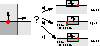
\includegraphics[width=0.75\textwidth]{pics/pdf/limitCategory.pdf}
  \caption[Illustration of limitation to of the algorithm to non-deep contacts.]{Illustration of limitation to of the categorization algorithm to non-deep contacts, since otherwise the collision arrangement is ambiguous, as shown by the possible arrangements a)-c).}
  \label{fig::limitCategory}
\end{figure}
 However, it is necessary to differentiate between the three cases in order to yield a distinct categorization since arrangements a) and c) are hooked collisions whereas b) is a regular collisions.
 As an interim solution we restricted the algorithm to non-deep collisions, thereby only arrangement a) is possible and the local arrangement is unambiguous. Furthermore, non-deep collisions are sufficient in many cases, since deep collisions often provide a visually unsatisfying result. 
  
 Nevertheless, the capability to handle deep contacts is desirable in order to simulate high-resolution meshes and to increase the overall robustness of the algorithm. To handle deep contacts additional information about the collision arrangement is required. This additional information could be provided by a global intersection analysis, similar to Baraff et al. \cite{BARAFF2003}, thereby it would be possible to differentiate between the sliding and the regular collisions for deep collisions. Alternatively, checking the neighbors of the new colliding vertex for collisions and taking their contact normals as a reference, would provide the necessary information and would provide less computational overhead.
 

\subsection{Redefinition of Feature Pairs}
\label{ss::redef}
%valid hier und valid by categories sollte unterscheidbar sein
To ensure plausible feature pairs and to avoid an inconsistent feature pair mapping, we trace the collisions and check each simulation step for possibly necessary redefinitions. A redefinition is possibly necessary if the first feature of the feature pair projected onto the second feature does not provide a geometrical overlap.
A redefinition is only "possibly" necessary since for concave surfaces it is possible that the projections of a feature do not overlap with any other feature. Imagine the 2D case of a vertex in the center of a five-pointed star, none of the sides overlaps with the projection of the vertex on the lines defined by the sides.

For VF collisions the assumption holds that as long as a vertex intersects a body, it is colliding with exact one face of the intersecting body. The redefinition for the VF case can be subdivided into two steps. The first step is to check if a redefinition is possibly necessary. If a redefinition is possibly necessary, we apply a second step and search for the correct face corresponding to the colliding vertex. 
An example of a VF redefinition is presented in figure \ref{fig::slidingVertexArtifactImplausibleForcesRedef} and in figure \ref{fig::svf_redef}.

In contrast to the VF case, no similar assumption holds for the EE case. An edge intersecting with another body can be colliding with one edge, with multiple edges or even with no edge.
Hence, there is no coherence between the elimination and new definition of a feature pair.
Therefore, the elimination and new definition are treated separately.
We check for eliminations at the end of each simulation step. For the new EE definitions we leverage that the new EE definitions go along with VF redefinitions.
Thus, we check for new EE definitions whenever we redefine a VF collision.

\begin{figure}[h] 
  \centering
     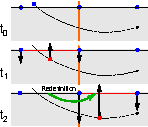
\includegraphics[width=0.40\textwidth]{pics/pdf/slidingVertexArtifactImplausibleForcesRedef.pdf}
  \caption[2D-Illustration of a barycentric redefinition.   Dots indicate the vertices, the red ones are colliding.]{2D-Illustration of a barycentric redefinition.   $t_0$ no collision, $t_1$ the single vertex is colliding with the left triangle, indicated red, $t_2$ the single vertex is now still colliding with the right triangle. The colliding face was redefined as indicated by the green arrow. The redefinition border is indicated with the orange-dotted line.}
  \label{fig::slidingVertexArtifactImplausibleForcesRedef}
\end{figure}


\begin{figure}[h!] 
\begin{minipage}[b]{0.5 \linewidth}
		\centering
		\subfigure[before the redefinition]{
			       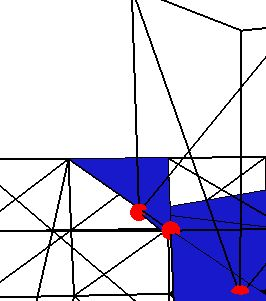
\includegraphics[width=0.4\linewidth]{pics/png/svf_redef_1.jpg} }
	\end{minipage}
	\begin{minipage}[b]{0.5 \linewidth}
		\centering
		\subfigure[after the redefinition]{
			       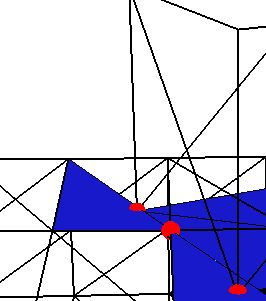
\includegraphics[width=0.4\linewidth]{pics/png/svf_redef_2.jpg} }
	\end{minipage}

  \caption[Example of a barycentric redefinition in a simulation.]{Example of a barycentric redefinition in a simulation. Subfigure a) shows the situation before the redefinition. Subfigure b) shows the same situation one time step later. The left vertex shifted under the next face, the collision is redefined and thereby updated to the next face .}
  \label{fig::svf_redef}
\end{figure}

\paragraph{Vertex Face Case}
For the VF case, we project the colliding vertex $V$ onto the plane of the colliding face $F$ and compute the barycentric coordinates $\omega_{fa}$, $\omega_{fb}$ and $\omega_{fc}$, see algorithm \ref{alg::VertexFaceFeaturePairRedefinition}.
The projected vertex is within the triangle if all barycentric weights are positive. Such collision pairs are considered valid and no redefinition is necessary.
Otherwise, it is possibly necessary to redefine the pair and we assume that the vertex went on to a face adjacent to the initial face.
With the direction information of the previously computed barycentric coordinates, we only need to check the faces adjacent to the vertices with positive weights.
Therefore, we project the vertex $V$ on the faces adjacent to vertices with positive weights.
 
Again, we check if the projected vertices are inside the new triangles by computing the barycentric weights.
All faces $F_i$ having only positive barycentric weights are candidates for the redefinition. In order the gain a regular collision, we apply the classification (see section \ref{ss::ContactCategorization}) and keep only the regular collisions as candidates. For the remaining candidates, we compute the penetration depths and choose the candidate with the smallest penetration depth. If no candidate was found, we do not redefine the collision.
 
To handle concave faces, we need to extend the algorithm.
For concave meshes it is possible that there is no face giving positive barycentric weights in the direct neighborhood. So we need to modify the barycentric weight condition. We define the barycentric tolerance $\varepsilon_v$ as
\begin{equation}
\varepsilon_v= \max\{
\begin{cases}
-\omega_i & \text{if } \omega_i<0 \\
\omega_i-1 &  \text{if } \omega_i>1\\
0&  \text{else}
\end{cases} \; | \; \omega_i \in \{\omega_a,\omega_b,\omega_c\}\}
\end{equation}
with the initial barycentric weights $\omega_{fa}$, $\omega_{fb}$ and $\omega_{fc}$.  $\varepsilon_v$ expresses the maximum discrepancy of the barycentric weights to the valid interval $[0,1]$.

In the algorithm we modify the condition for redefinition candidates. We now do not only add all vertices having all their barycentric coordinates in the interval $[0,1]$, but also the vertices in the interval $[-\varepsilon_v,1+\varepsilon_v]$.




\begin{algorithm}                    % enter the algorithm environment
\caption{Vertex Face Feature Pair Redefinition for convex meshes}          % give the algorithm a caption
\label{alg::VertexFaceFeaturePairRedefinition}                           % and a label for \ref{} commands later in the document
\begin{algorithmic}[1]                    % enter the algorithmic environment
    \STATE Input: Vertex V, Face F, List Collisions, List ResolvedCollisions,  $\omega_{FA}$, $\omega_{FB}$, $\omega_{FC}$, $n_F$
    \STATE Result:  List Collisions, List ResolvedCollisions
    	\STATE List RedefinitionCandidates
        \IF{$\omega_{FA}>0$}
           	\STATE RedefinitionCandidates.add(neighbouringFaces($V_A$))
        \ENDIF
        \IF{$\omega_{FB}>0$}
          	\STATE RedefinitionCandidates.add(neighbouringFaces($V_B$))    
        \ENDIF
        \IF{$\omega_{FC}>0$}
	        \STATE RedefinitionCandidates.add(neighbouringFaces($V_C$)) 
       	\ENDIF
       	\STATE currentBestDepth $=-\infty$ 
       	\STATE Collision currentCollision
       	\FORALL{Face $F_i$ in RedefinitionCandidates}
       	 	\STATE $\omega_{IA}$, $\omega_{IB}$, $\omega_{IC}$ $ \Leftarrow$ computedProjectedBarycentrics(V,$F_i$)       	  	
	        \IF{$\omega_{IA}>0 \land \omega_{IB}>0 \land \omega_{IC}>0$}
	        \IF{regular==collisontype(Collision(V,$F_i$))}
     	       	\STATE $n_i =$faceNormal($F_i$) 
     	    	\STATE $d_i$ =penetrationdepth(V,$F_i)$
	        	\IF{$d_i>$currentBestDepth $\land$ $d_i<0$)}
					\STATE currentBestDepth$=d_i$
					\STATE currentCollision$=$Collision(V,$F_i$)				
							  		\ENDIF 			
							  				  		\ENDIF 
	     	\ENDIF
        \ENDFOR
     	\IF{currentBestDepth$>-\infty$}
	     	\STATE Collisions.add(currentCollision)
	     	\STATE ResolvedCollisions.add(Collision(V,F))
     	\ENDIF
\end{algorithmic}
\end{algorithm}


\paragraph{Edge Edge Case} For the EE case, in each simulation step before we compute the collision impulses, we check whether the collision needs to be dismissed. Therefore, we project the edge $E_B$ on the plane defined by the Edge $E_A$ with the contact normal as plane and projection normal. We compute the barycentric coordinates $\omega_{A0}$, $\omega_{A1}$, $\omega_{B0}$ and $\omega_{B1}$  of the point of intersection between the projected $E_A$ with $E_B$.
If the edges overlap, all barycentric coordinates are positive and the collision will be handled.
To avoid the missing of EE collisions, we apply a relaxed condition; if the barycentric weights are in the interval $[-\varepsilon_E,1+\varepsilon_E]$ with $\varepsilon_E=0.3$ the collision is kept, but not handled. For the case that not even the relaxed condition is fulfilled, the collision is dismissed.

Due to the circumstance that there is not always a coherence between the dismissing of an EE collision and the appearance of a new EE collision, checking the dismissed edges' neighbors is not sufficient for an accurate EE redefinition.
In consideration of the circumstance that EE redefinitions go along with VF redefinitions we couple the EE redefinitions to the VF redefinitions instead of EE dismissals.

We consider a VF redefinition of a vertex $V_S$ which is redefined from the face $F_{old}$ with the face normal $n_{ref}$ to the adjacent face $F_{new}$. All neighboring edges of $V_S$ are saved in a candidate list $L_A$. All edges adjacent to at least one of the mutual vertices of  $F_{old}$ and $F_{new}$ are saved in a second candidate list $L_B$. 

%Both lists are filtered to ensure plausible feature pairs.
%For $L_A$ we only allow edges with a surface normal span showing in the opposite direction of $n_{ref}$ and the edge vector orthogonal to $n_{ref}$. For $L_B$ the filter is similar, except that surface normal span has to show in the same direction as $n_{ref}$.
 
We test all possible EE feature pairs for new collisions, by testing each edge in $L_A$  against each edge in $L_B$. If a feature pair is according to section \ref{ss::ContactCategorization} regular and the projected barycentric coordinates are in the relaxed interval $[-\varepsilon_E,1+\varepsilon_E]$ we keep the feature pair as a collision.


\subsection{Redefinition of Hooked Contacts}
\label{ss::sliding}

We consider hooked collisions as aberrant and correct these collisions.
A nearby attempt would be to directly modify the direction of the collision impulse.
However, the direction is defined by the contact normal, which is an essential element of the CPF algorithm. Therefore, we redefine the hooked collision pairs in order to reduce the tangential impulses and to gain regular collision pairs, as shown in figure \ref{fig::slidingVertexArtifactDiscretizationForcesRedef}.
For the EE case these redefinitions are already covered by the collision redefinition in section \ref{ss::redef}. 
For the VF case we handle the hooked contacts with a redefinition of the feature pair similar to the implausible feature pairs case, see section \ref{ss::redef}.
In contrast to the implausible feature pairs case, the barycentric weights for the initial face generally are positive.
This allows us to use algorithm \ref{alg::VertexFaceFeaturePairRedefinition} with only a small change in the first step. We now search in all triangles adjacent to the triangle vertices and not only the triangles adjacent to vertices with positive weights. This change is necessary since we do not have a direction information, as in the case of barycentric redefinition provided by violation of [0,1] interval by the barycentric weights. 

\begin{figure}[h] 
  \centering
     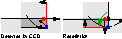
\includegraphics[width=0.70\textwidth]{pics/pdf/slidingVertexArtifactDiscretizationForcesRedef.pdf}
  \caption[2D-Illustration of the redefinition for a hooked collision.]{2D-Illustration of the redefinition for a hooked collision. The redefinition is marked with a green arrow. Before the redefinition, the red face collides with the surface vertex of the lower body resulting in forces almost tangential to the surface of the lower body and reverting the tangential movement. After the redefinition, the vertex collides with the redefined bottom sided face, resulting in forces in the normal direction of the lower surface and the tangential movement is preserved.}
  \label{fig::slidingVertexArtifactDiscretizationForcesRedef}
\end{figure}

In sum, the redefinition algorithm for a hooked collision can be reduced to four (simplified) steps (see figure \ref{fig::slidingVertexArtifactDiscretizationForcesRedefAlgo}). In the first step, the triangles adjacent to the colliding triangle are saved as candidates. In the second step, the colliding vertex is projected onto the planes defined by the candidate triangles and it is checked whether the projection is inside the triangles. All candidates with the projection outside the triangle are dismissed. In the third step, the remaining candidates are tested for artifact collisions and all candidates which would yield artifact collisions are dismissed. In the fourth and final step, generally, only one triangle is left. However, it is possible that multiple triangles are left therefore we choose the candidate with the smallest intersection for the redefinition. 

\begin{figure}[h] 
  \centering
     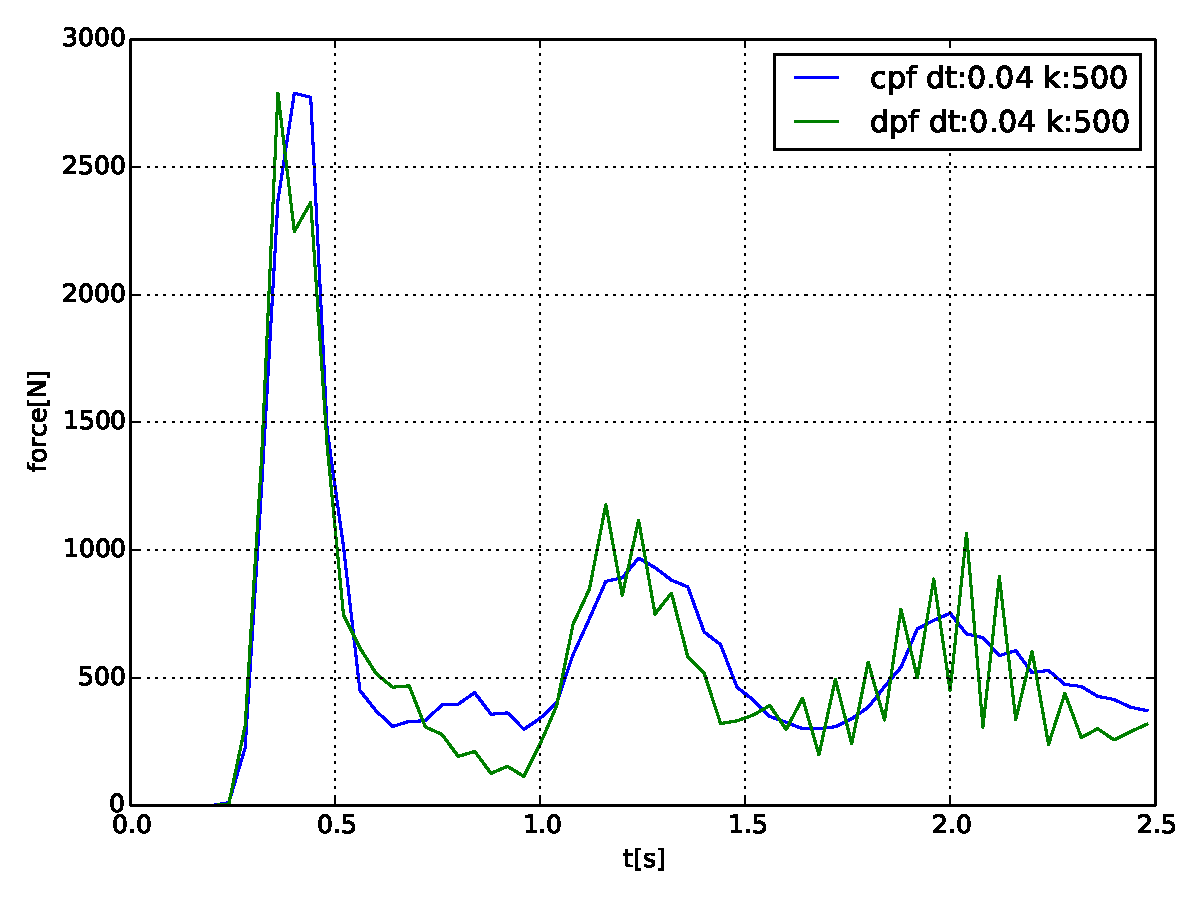
\includegraphics[width=1.0\textwidth]{pics/pdf/slidingVertexArtifactDiscretizationForcesRedefAlgo.pdf}
  \caption[2D-Illustration of the redefinition for a hooked collision.]{2D-Illustration of the redefinition for a hooked collision. 1) Neighboring triangles are candidates 2) Dismissal of the candidates with the vertex projection outside the triangle 3) Dismissal of the artifact candidates 4) Redefinition to the final candidate}
  \label{fig::slidingVertexArtifactDiscretizationForcesRedefAlgo}
\end{figure}

\chapter{Results}
\label{ch:results}
In this chapter, we analyze the CPF algorithm and discuss the results in comparison to a DPF algorithm. Furthermore, we analyze and discuss the newly introduced contact redefinition and the friction formulation under use of varying parameters and scenarios.


%Furthermore, for interactive systems it is important to simulate large timesteps and to provide low computational costs to reach high frame rates.

We will begin with the analysis of a 1D particle on plane contact, providing the possibility to formulate the integration scheme and compute the stable time steps in an analytic fashion.
Thereafter, we will apply the preliminary findings to investigate a more complex scenario, the collision between a deformable bar and a rigid cube with a focus on stability, jitter and penetration depth. 
Afterwards, we will examine the applied friction model regarding static and dynamic friction.
Subsequently, we will show the results of the introduced contact redefinition algorithm and discuss the benefits.
Finally, we will investigate the overall computational cost of the collision resolution with a special regard to the additional cost induced by the new redefinition algorithm.

In order to provide a matchable result of the comparison of DPF and CPF, in all tests DPF are computed with CCD using the penetration depth at t=1.
\section{Stability}
\label{sec::stability}
In general, it is difficult to measure the correct behavior of a multi-body simulation, since it only provides physically plausible instead of physically exact results. Therefore, we need to couple an analytical and visual evaluation.

An essential property for collision handling methods is stability. Otherwise, the energy in the system increases and collision resolutions provide irritating results. Furthermore, jitter and deep intersections disturb the visual impression.

\subsection{Analysis of 1D Particle-on-Plane Contact}
The analysis of a 1D particle-on-plane contact provides the possibility to describe the scenario in an analytical way, which is not feasible for more complex scenarios.
The analytical description allows us to apply analytical methods to evaluate the stability. Afterwards, we will validate these findings in the simulation of the particle and the simulation of a more complex scenario.

The continuous motion of a particle heading towards a plane under gravity can be described as
\begin{align}
\dot x &=v \\
 \dot v &=
\begin{cases}
-g-\frac{kx}{m} & \text{ if } x<0 \\
-g & \text{ else }
\end{cases}
\end{align}
with the gravity coefficient $g$, the mass $m$, the penalty stiffness $k$, the position $x$ and the velocity $v$. The particle only moves up and down, therefore the movement can be expressed in 1D and all quantities are scalars.  As in the simulation the equation needs to be discretized in time with a time step $\Delta t$ in a form of
\begin{equation}
\label{eq::update_form}
	\begin{pmatrix}
		x(t+\Delta t) \\
		v(t+\Delta t) 
	\end{pmatrix}=\mathbf A
		\begin{pmatrix}
			x(t) \\
			v(t) 
		\end{pmatrix},
\end{equation}
where the matrix $\mathbf A$ describes the integration scheme. The integration scheme is stable if all eigenvalues $\lambda$ satisfy $|\lambda(\mathbf{A})|<1$.

Discrete penalty forces (see section \ref{sec:DiscretePF}) compute the collision impulse as
\begin{equation}
I_{dpf}=-\Delta t kx^*(t+\Delta t)
\end{equation}
with the predicted position $x^*(t+\Delta t)=x(t)+\Delta t  v^*(t+\Delta t)$ and the predicted velocity $v^*(t+\Delta t)$, which is $v^*(t+\Delta t)=v(t)$ neglecting gravity. The update rule yields
\begin{align}
	v(t+\Delta t)&=v(t)+\frac{I_{dpf}}{m}=v(t)-\Delta t \frac{k}{m} x(t)-\Delta t^2 \frac{k}{m} v(t) \\
	x(t+\Delta t)&=x(t)+\Delta t v(t+\Delta t)	
\end{align}
and in matrix form it is
\begin{equation}
	\begin{pmatrix}
		x(t+\Delta t) \\
		v(t+\Delta t) 
	\end{pmatrix}=	
		\begin{pmatrix}
			1-\Delta t^2\frac{k}{m} \ \ \Delta t - \Delta t^3\frac{k}{m}  \\
		-\Delta t\frac{k}{m} \ \ 1- \Delta t^2 \frac{k}{m}
		\end{pmatrix}
		\begin{pmatrix}
			x(t) \\
			v(t) 
		\end{pmatrix}.
\end{equation}
The eigenvalues analysis gives stable time-steps for $\Delta t< \sqrt{\frac{4}{3}\frac{m}{k}}$.

Continuous penalty forces (see section \ref{sec:ContinuousPenaltyForces}) compute the collision impulse as
\begin{equation}
I_{cpf}=-\Delta t kx(t)-\frac{\Delta t^2}{2} kv^*(t+\Delta t)
\end{equation}
with the predicted velocity $v^*(t+\Delta t)=v(t)$. The update rule yields
\begin{align}
	v(t+\Delta t)&=v(t)+\frac{I_{cpf}}{m}=v(t)-\Delta t \frac{k}{2m} x(t)-\Delta t^2 \frac{k}{m} v(t) \\
	x(t+\Delta t)&=x(t)+\Delta t v(t+\Delta t)	
\end{align}
and matrix form it is
\begin{equation}
	\begin{pmatrix}
		x(t+\Delta t) \\
		v(t+\Delta t) 
	\end{pmatrix}=	
		\begin{pmatrix}
			1-\Delta t^2\frac{k}{m} \ \ \Delta t - \Delta t^3\frac{k}{2m}  \\
		-\Delta t\frac{k}{m} \ \ 1- \Delta t^2 \frac{k}{2m}
		\end{pmatrix}
		\begin{pmatrix}
			x(t) \\
			v(t) 
		\end{pmatrix}
\end{equation}
The eigenvalues analysis yields stable time-steps for $\Delta t< \sqrt{2 \frac{m}{k}}$.

Comparing the stable time steps shows that the maximum time step size for CPF is $\frac{\sqrt{6}}{2}\approx1.22$ times larger than for DPF.

To verify the previous theoretical consideration, we analyze a particle with a mass $m=1.0kg$ and a starting height $h=0.1m$ dropped on the plane  with a penalty coefficient $k=100.0\frac{N}{m}$.
According to the previous formula the critical step size for CPF is $\Delta t_{cpf}=\sqrt{0.02}s\approx0.142s$ and for DPF $\Delta t_{dpf}=\sqrt{\frac{4}{300}}s\approx0.115s$.
As shown in figure \ref{fig::particle_multdt}, CPF are stable for $\Delta t=0.14<\Delta t_{cpf}$ damping the initial deflection and unstable for $\Delta t=0.17>\Delta t_{cpf}$ amplifying the initial deflection.
Similarly, the DPF are stable for $\Delta t=0.11<\Delta t_{dpf}$  and unstable for $\Delta t=0.13>\Delta t_{dpf}$.

As predicted by the stability analysis, the CPF are, for the particle-plane case, stable for larger time steps than DPF. We show that CPF are stable for $\Delta t=0.14$ whereas the discrete penalty forces are already unstable for $\Delta t=0.13$.

\begin{figure}[h!]
	\begin{minipage}[b]{0.5 \linewidth}
		\centering
		\subfigure[CPF with $\Delta t=0.14s$]{
			       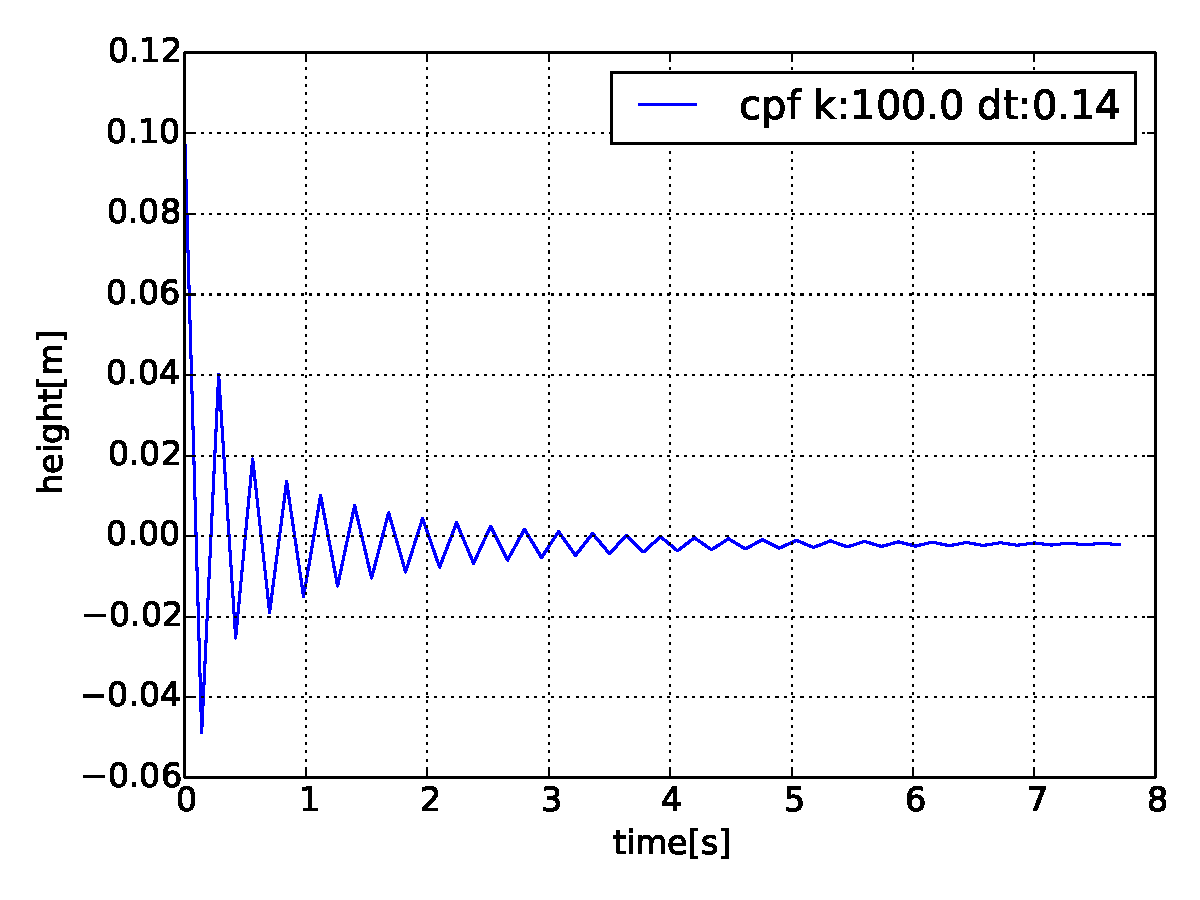
\includegraphics[width=1.0\linewidth]{pics/pdf/particle_cpf_k100dt014.pdf} }
	\end{minipage}
	\begin{minipage}[b]{0.5 \linewidth}
		\centering
		\subfigure[CPF with $\Delta t=0.17s$]{
			       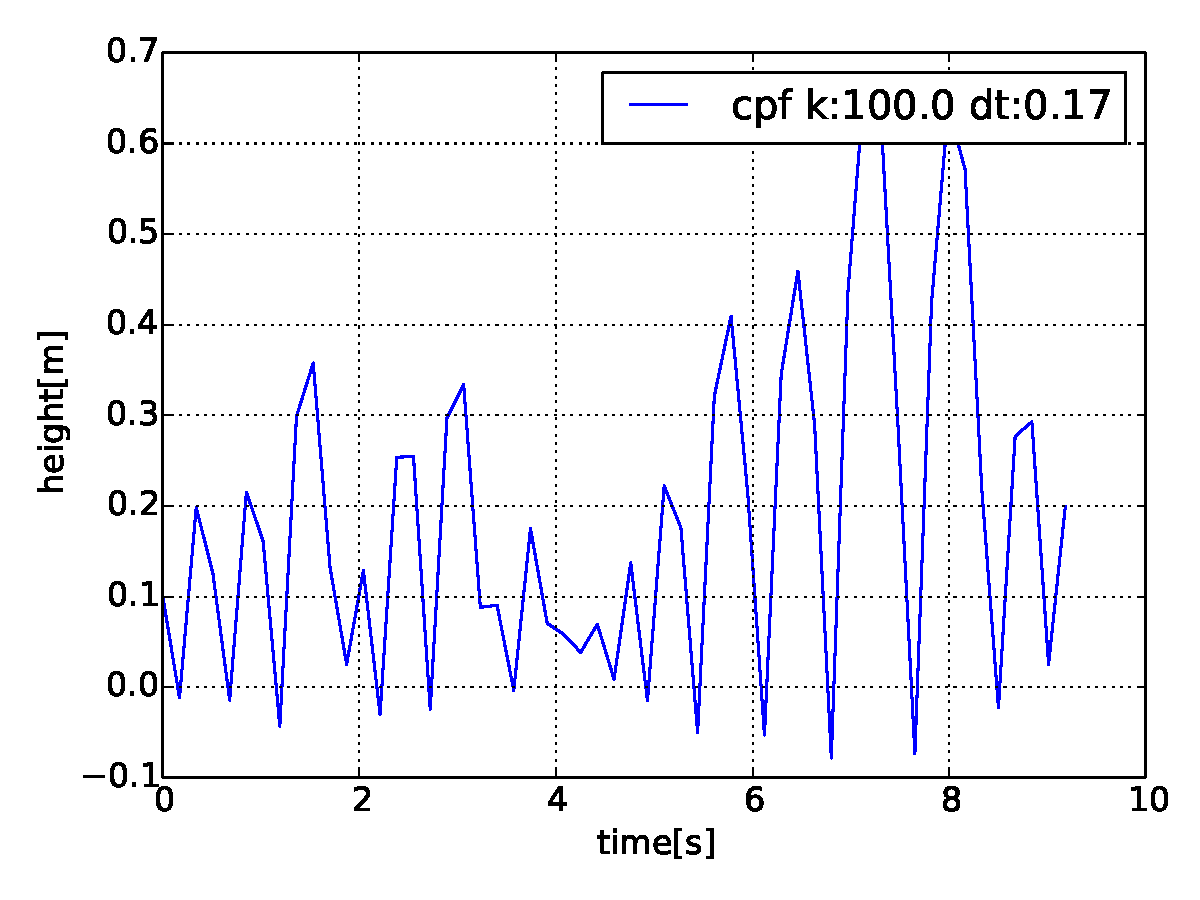
\includegraphics[width=1.0\linewidth]{pics/pdf/particle_cpf_k100dt017.pdf} }
	\end{minipage}\\
	
		\begin{minipage}[b]{0.5 \linewidth}
			\centering
			\subfigure[DPF with $\Delta t=0.11s$]{
				       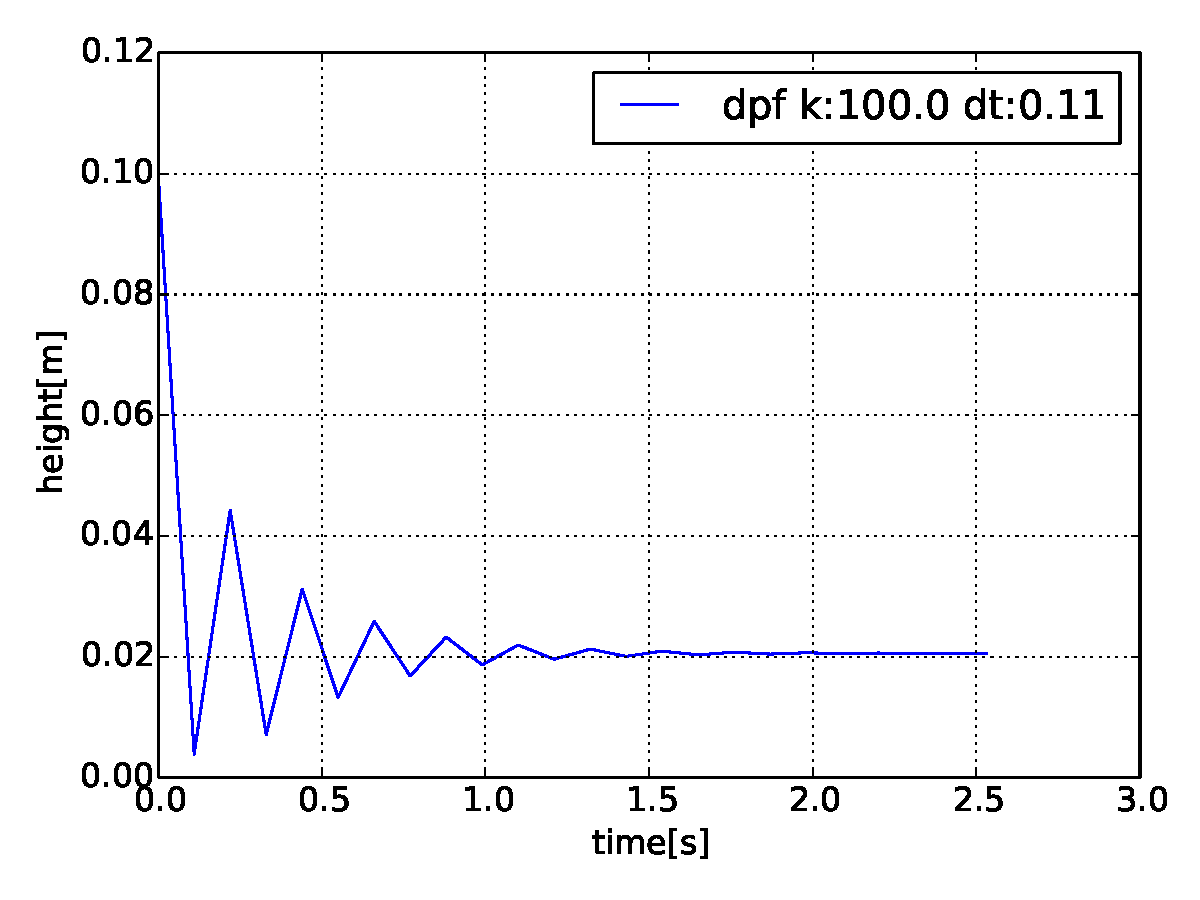
\includegraphics[width=1.0\linewidth]{pics/pdf/particle_dpf_k100dt011.pdf} }
		\end{minipage}
		\begin{minipage}[b]{0.5 \linewidth}
			\centering
			\subfigure[DPF with $\Delta t=0.13s$]{
				       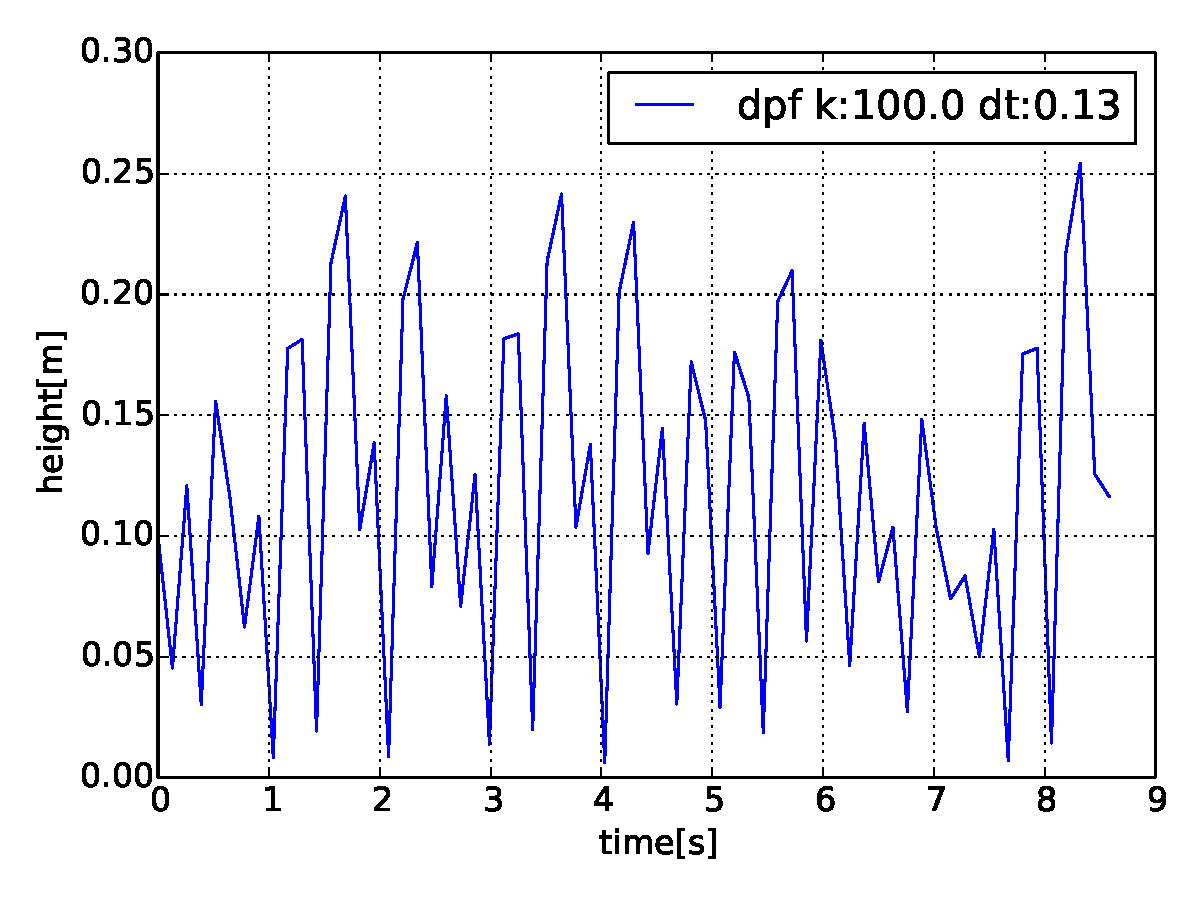
\includegraphics[width=1.0\linewidth]{pics/pdf/particle_dpf_k100dt013.pdf} }
		\end{minipage}	
\caption[The position over time of a particle m=1.0kg  dropped from h=0.1m on a plane with continuous (a, b) and discrete (c, d) penalty forces]{The position over time of a particle m=1.0kg  dropped from h=0.1m on a plane with continuous (a, b) and discrete (c, d) penalty forces, showing stable (a, c) and unstable (b, d) conditions. It is noticeable that CPF are stable for $\Delta t=0.14$ whereas the discrete penalty forces are already unstable for $\Delta t=0.13$.}
\label{fig::particle_multdt}
\end{figure}

Stability is an essential property for interactive environments. With the relation for stable time steps $\Delta t< \sqrt{2 \frac{m}{k}}$, stability can be ensured by choosing lower penalty coefficients $k \ll 2\frac{m}{\Delta t^2}$.
Since this is a common case, we again analyze the movement of a particle $m=1.0kg$ and a starting height $h=0.1m$ with a time step $\Delta t=0.01s$ and penalty coefficient $k=1000.0\frac{N}{m} \ll 2 \frac{1.0}{0.01^2}\frac{N}{m}=20000\frac{N}{m}$. 
The result is shown in figure \ref{fig::particle_samedt}.
Figure \ref{fig::particle_samedt} a) shows the movement of the particle with DPF and CPF.
Both methods show likewise results, damping the initial deflection, but the DPF damping is considerably larger than the CPF damping.
As a result the CPF particle keeps bouncing for a longer time.
The damping is induced by the reason that both methods overestimate the penetration depth as long as the penetration depth is increasing, resulting in an increased deceleration. Similarly, both methods underestimate the penetration depth when the penetration depth is decreasing, resulting in a reduced acceleration of the particle, as described in section \ref{sec:CPFGENERAL}.

CPF take the particle trajectory into account, therefore the estimation error is smaller and subsequently the damping is reduced.

\begin{figure}[tbp] 
\begin{minipage}[b]{0.5 \linewidth}
		\centering
		\subfigure[Movement of the particle]{
			       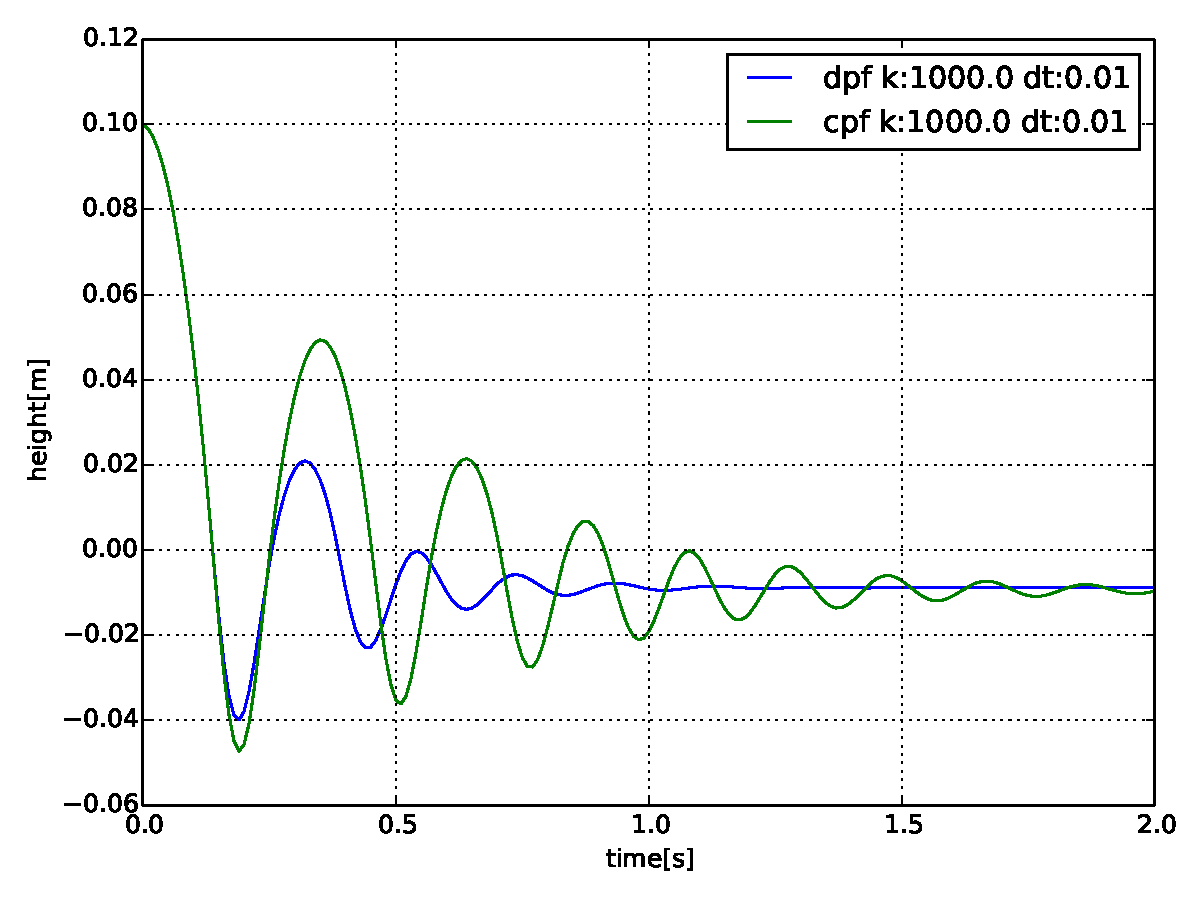
\includegraphics[width=1.0\linewidth]{pics/pdf/particle_k1000dt001.pdf} }
	\end{minipage}
	\begin{minipage}[b]{0.5 \linewidth}
		\centering
		\subfigure[Forces during the first collision]{
			       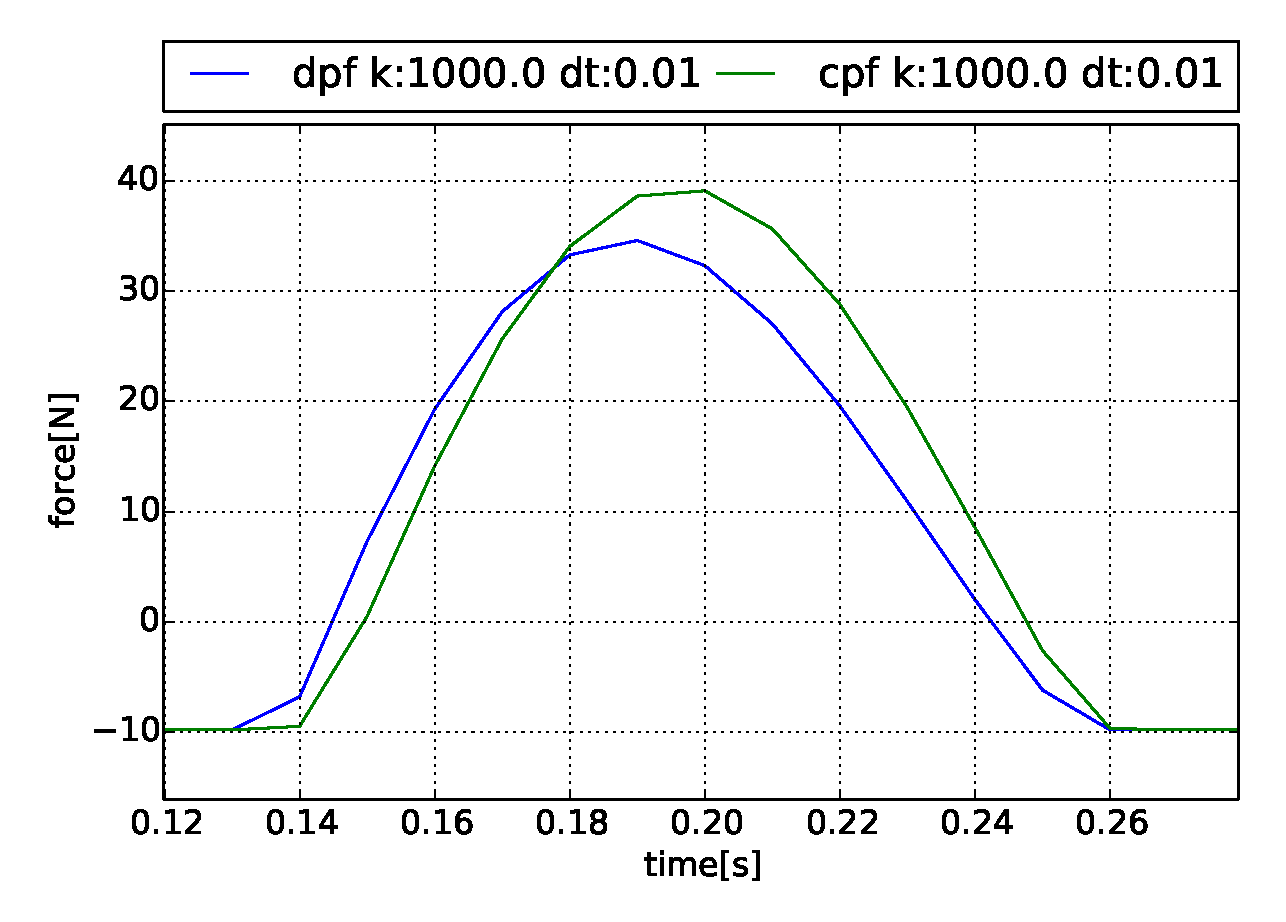
\includegraphics[width=1.0\linewidth]{pics/pdf/particle_k1000dt001_f.pdf} }
	\end{minipage}

  \caption{The position over time of a particle dropped on a plane with continuous and discrete penalty forces with the same time step $\Delta t=0.01$ and penalty stiffness $k=1000$}
  \label{fig::particle_samedt}
\end{figure}

The analytical evaluation of the 1D-particle-plane contact has shown that for CPF the maximum stable timestep is $\frac{\sqrt{6}}{2}\approx1.22$ times larger than the maximum stable timestep for DPF.
The result could be validated in the simulation. Furthermore, the simulation has shown less damping for the CPF. Overall, we have seen two benefits of CPF in comparison to DPF, increased stability and reduced damping. The according computational cost is analyzed in section \ref{sec:compCost}.

\subsection{Deformable Bar vs Rigid Cube}
The particle-on-plane scenario provides an analytical description of the algorithms, what is not feasible for more complex scenes.
However, due to the static plane the overall CPF computation reduces from a degree 6 polynomial to a quadratic polynomial. To investigate the validity of the previous findings for more complex scenarios, we analyze a scenario with a rotated deformable bar dropped on a rigid cube which again is dropped on the ground, as shown in figure \ref{fig::defCubeVsBar}. Furthermore, the scenario is set up in a fashion to avoid the artifacts presented in section \ref{sec::stability}.

 \begin{figure}[h!] 
 \begin{minipage}[b]{0.33 \linewidth}
 		\centering
 		\subfigure[3D flat shaded]{
 			       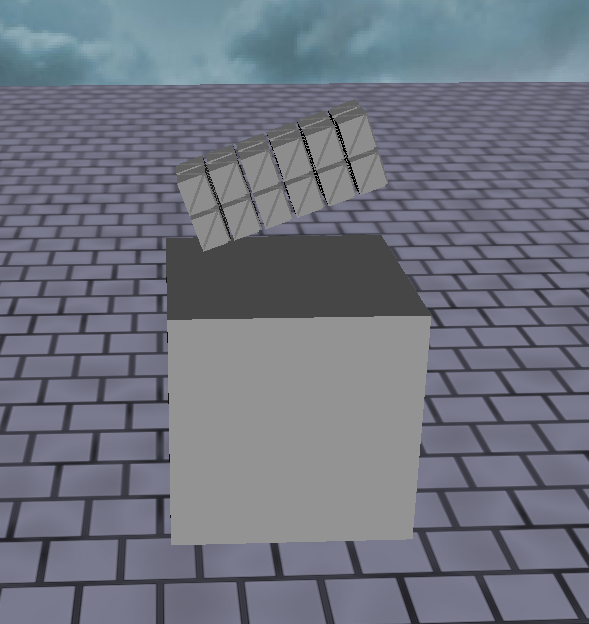
\includegraphics[width=0.95\linewidth]{pics/png/barvscube_rend.png} }
 	\end{minipage}
 	\begin{minipage}[b]{0.33 \linewidth}
 		\centering
 		\subfigure[3D wireframe]{
 			       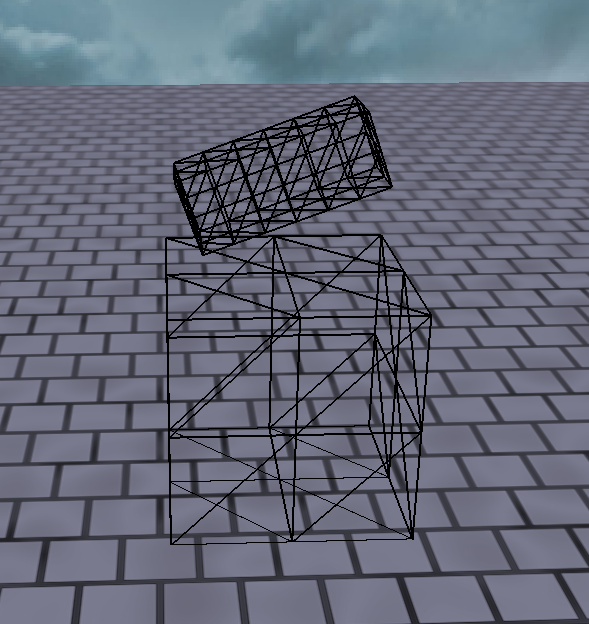
\includegraphics[width=0.95\linewidth]{pics/png/barvscube_wf.png} }
 	\end{minipage}
 	 	\begin{minipage}[b]{0.33 \linewidth}
 	 		\centering
 	 		\subfigure[2D from top]{
 	 			       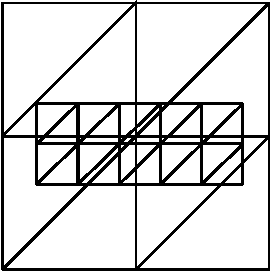
\includegraphics[width=0.95\linewidth]{pics/pdf/cube_bar_discretization.pdf} }
 	 	\end{minipage}
 
   \caption[Illustration of discretizations of the deformable bar on the rigid cube.]{Illustration of discretizations of the deformable bar on the rigid cube. In the center of the bar more features are overlapping than at the edging and thus there are more feature collisions.}
   \label{fig::defCubeVsBar}
 \end{figure}
 
 \begin{figure}[h!] 
 \begin{minipage}[b]{0.50 \linewidth}
 		\centering
 		\subfigure[Repulsion force with DPF ]{
        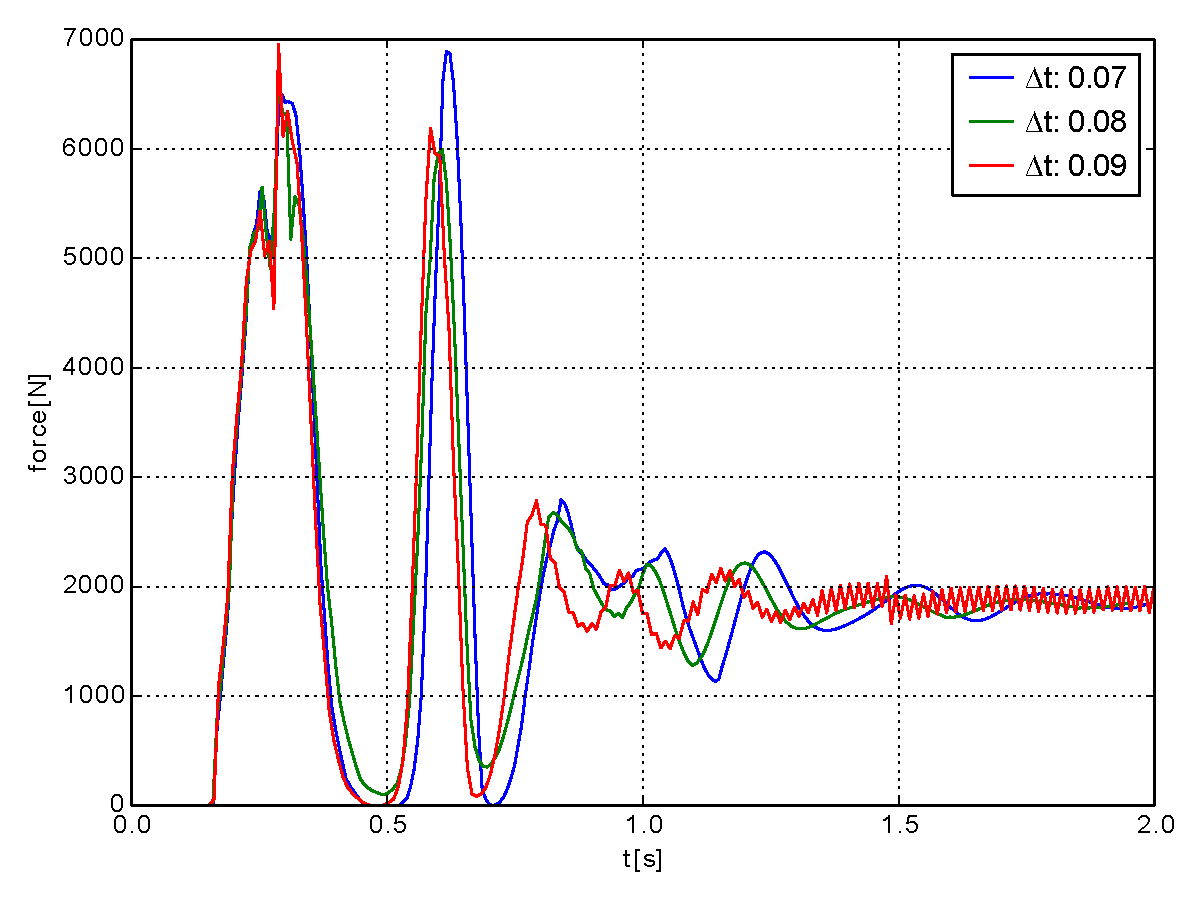
\includegraphics[width=1.0\linewidth]{pics/pdf/cubeBlockBM_dt_dpf.pdf} }
 	\end{minipage}
 	\begin{minipage}[b]{0.50 \linewidth}
 		\centering
 		\subfigure[Repulsion force with CPF]{
        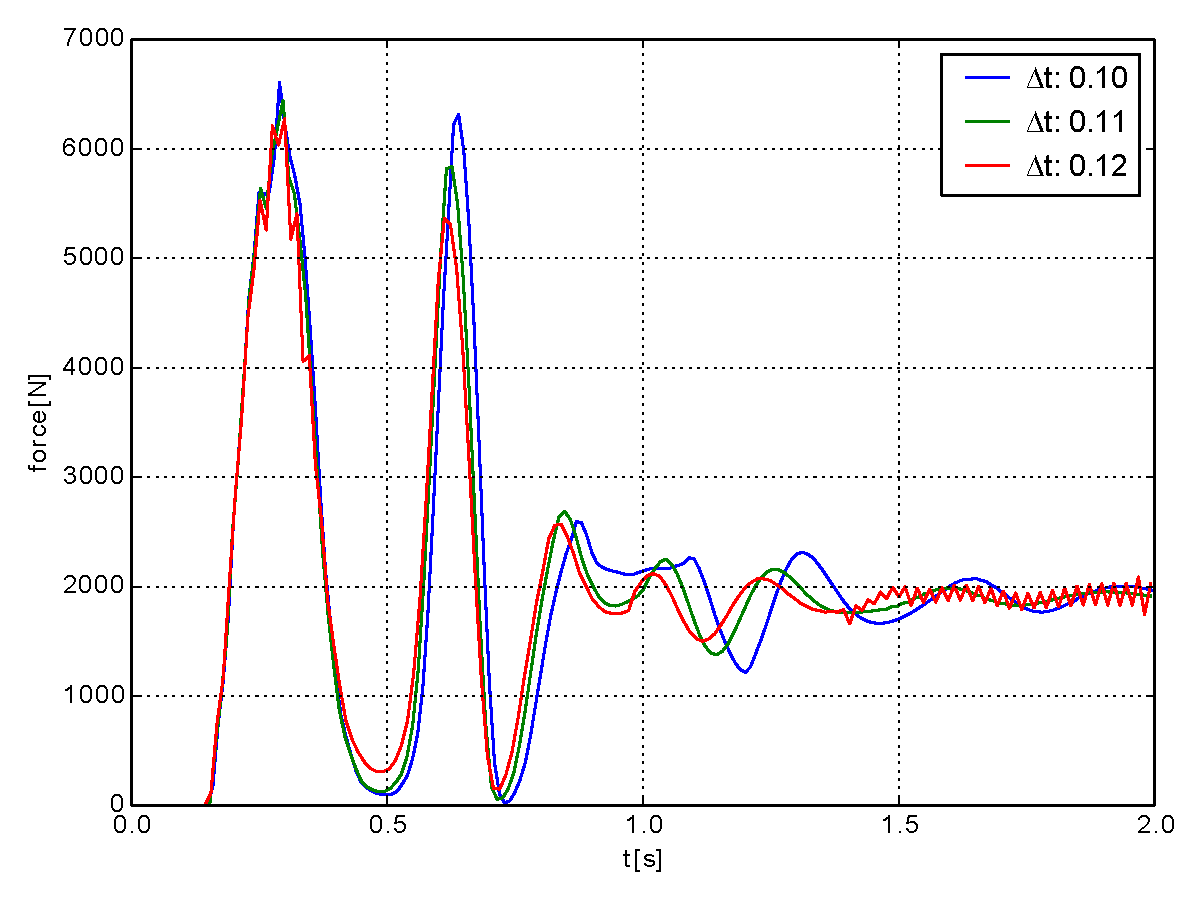
\includegraphics[width=1.0\linewidth]{pics/pdf/cubeBlockBM_dt_cpf.pdf} }
 	\end{minipage}
 \caption[Comparison of the repulsion force between a deformable bar and a rigid cube with varying time steps $\Delta t$ and and constant penalty coefficients $k=5000$.]{Comparison of the repulsion force between a deformable bar and a rigid cube with varying time steps $\Delta t$ and and constant penalty coefficients $k=5000$. The left plots show the force with DPF and jitter can be noted for $\Delta t=0.009$, whereas for the plots on right side with CPF jitter can be initially noted for a larger time step $\Delta t=0.012$}
 \label{fig::BlockBM_dt}
 \end{figure} 

We set the penalty coefficient to $k=5000$ and vary the time step sizes. % and examined the first to seconds whereupon the deformable bar rests on the rigid cube.
DPF resolve the collisions without notable jitter for time steps up to $\Delta t_d=0.08$, whereas CPF are smooth for time steps up to $\Delta t_c=0.11$. This matches roughly the ratio of 1.22 predicted in the particle-on-plane analysis.
The jitter observed in simulation is also notable in the plot of the collision forces between the cube and the bar as shown in figure \ref{fig::BlockBM_dt}.
Figure \ref{fig::BlockBM_dt} a) shows the DPF repulsion forces for time steps sizes $\Delta t=0.007s$, $\Delta t=0.008s=\Delta t_d$, $\Delta t=0.009s$ and figure \ref{fig::BlockBM_dt} b) shows the CPF repulsion forces for time steps sizes $\Delta t=0.010s$, $\Delta t=0.011s=\Delta t_c$, $\Delta t=0.012s$.
The overall plots are similar, there are two large peaks in the beginning at $t=0.3s$ and $t=0.6s$ with high repulsion forces when the deformable bar collides with the rigid cube and is pushed up again.
From $t\approx0.8s$ on the bar tumbles on the block, arising as a damped oscillation. There is a jitter notable in the force process for the higher time steps of each method.
For DPF, especially for $\Delta t=0.009$, it is notable from $t=0.7$ on and for CPF  it is notable for $\Delta t=0.012$ from $t=1.4$ on. This jitter in the force plot is also optically notable as jitter in the movement of vertices.
 

The jitter mainly takes place at the vertices in the middle of the bottom side of the bar, since there are more feature collisions than at the physical edges due to the discretization of the cube as shown in figure \ref{fig::defCubeVsBar} c).
In the center of the bar, more features overlap than at the physical edge and thus there are more feature collisions.\\
In sum we have seen that also for a more complex scenario CPF provide stability for larger time steps and validated the results from the particle-plane scenario.\\
Up to now the penalty coefficient was constant and we varied the time step.
In the following we vary both, the time step and the penalty coefficient to reach a comprehensive comparison of the CPF and DPF.\\
We chose multiple time steps $\Delta t$ and in order he provide stable simulations compute $k$ according to the relation $\Delta t \sim \sqrt{\frac{m}{k}}$ from the 1D particle analysis. 
The resulting forces are shown in figure \ref{fig::defBar_vs_RigCubeBM}.
For all four cases, CPF provide a much smoother force curve than the DPF. Again, it is also notable in the simulation since there is a notable jitter for DPF.\\ 
\begin{figure}[tp] 
\begin{minipage}[b]{0.5 \linewidth}
		\centering
		\subfigure[$\Delta$t=0.005, k=20000]{
			       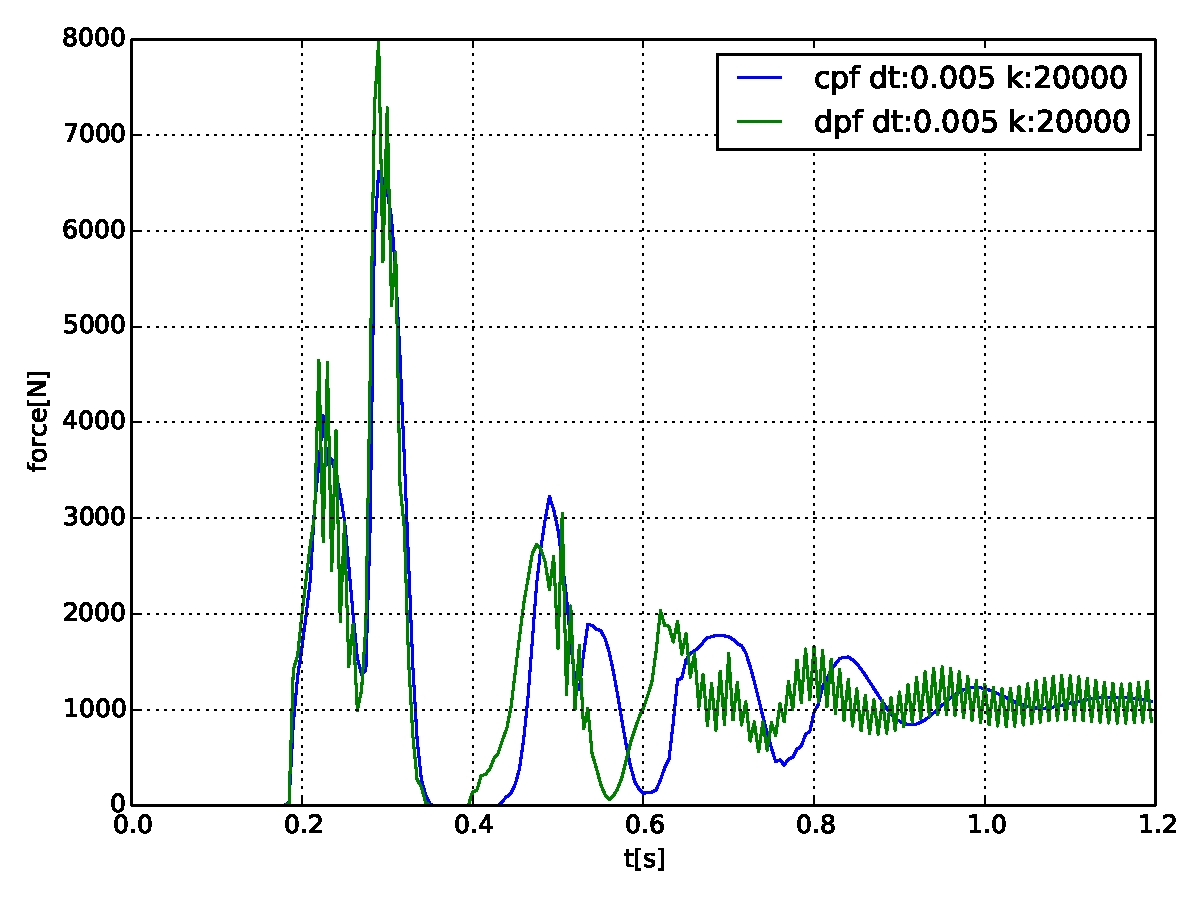
\includegraphics[width=1.0\linewidth]{pics/pdf/cubeBM_t0005.pdf} }
	\end{minipage}
	\begin{minipage}[b]{0.5 \linewidth}
		\centering
		\subfigure[$\Delta$t=0.01, k=5000]{
			       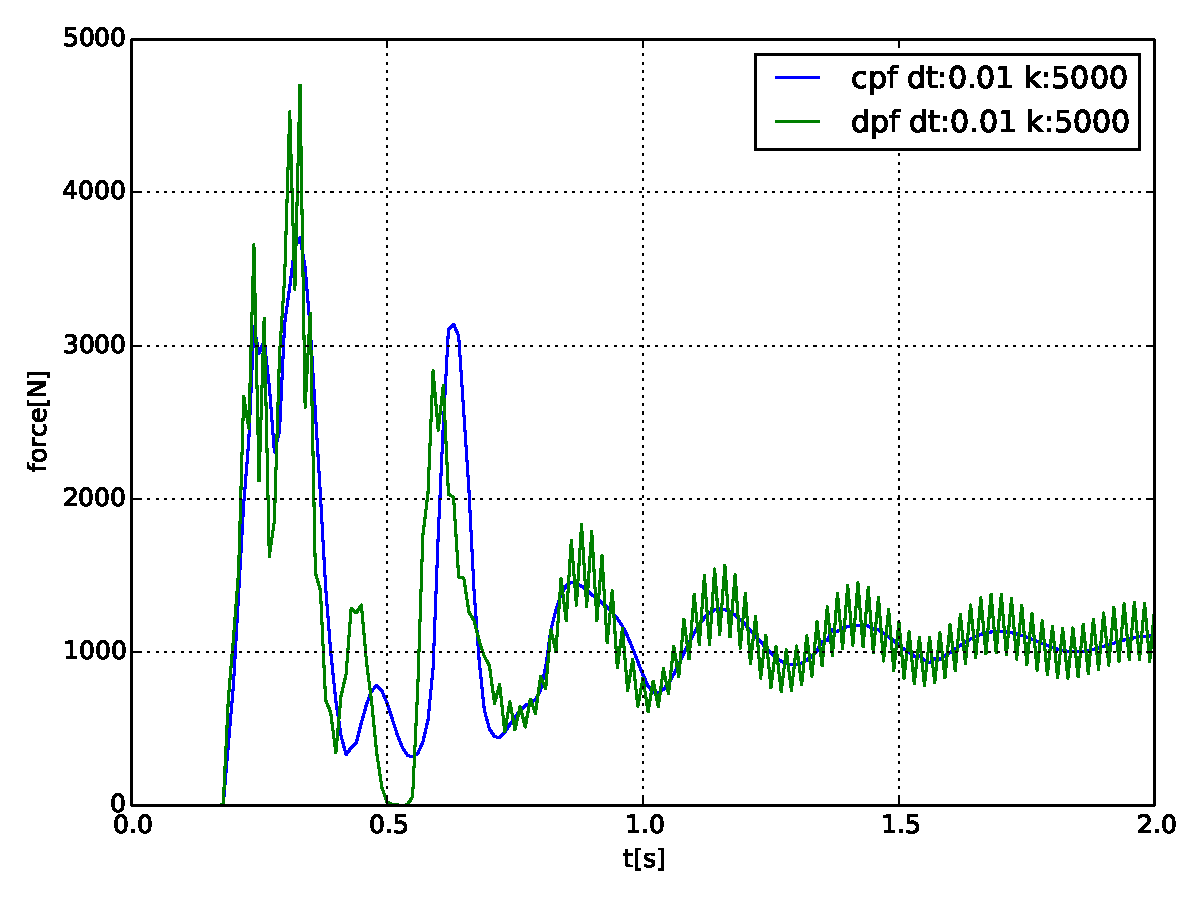
\includegraphics[width=1.0\linewidth]{pics/pdf/cubeBM_t001.pdf} }
	\end{minipage}\\	
	\begin{minipage}[b]{0.5 \linewidth}
			\centering
			\subfigure[$\Delta$t=0.02, k=1250]{
				       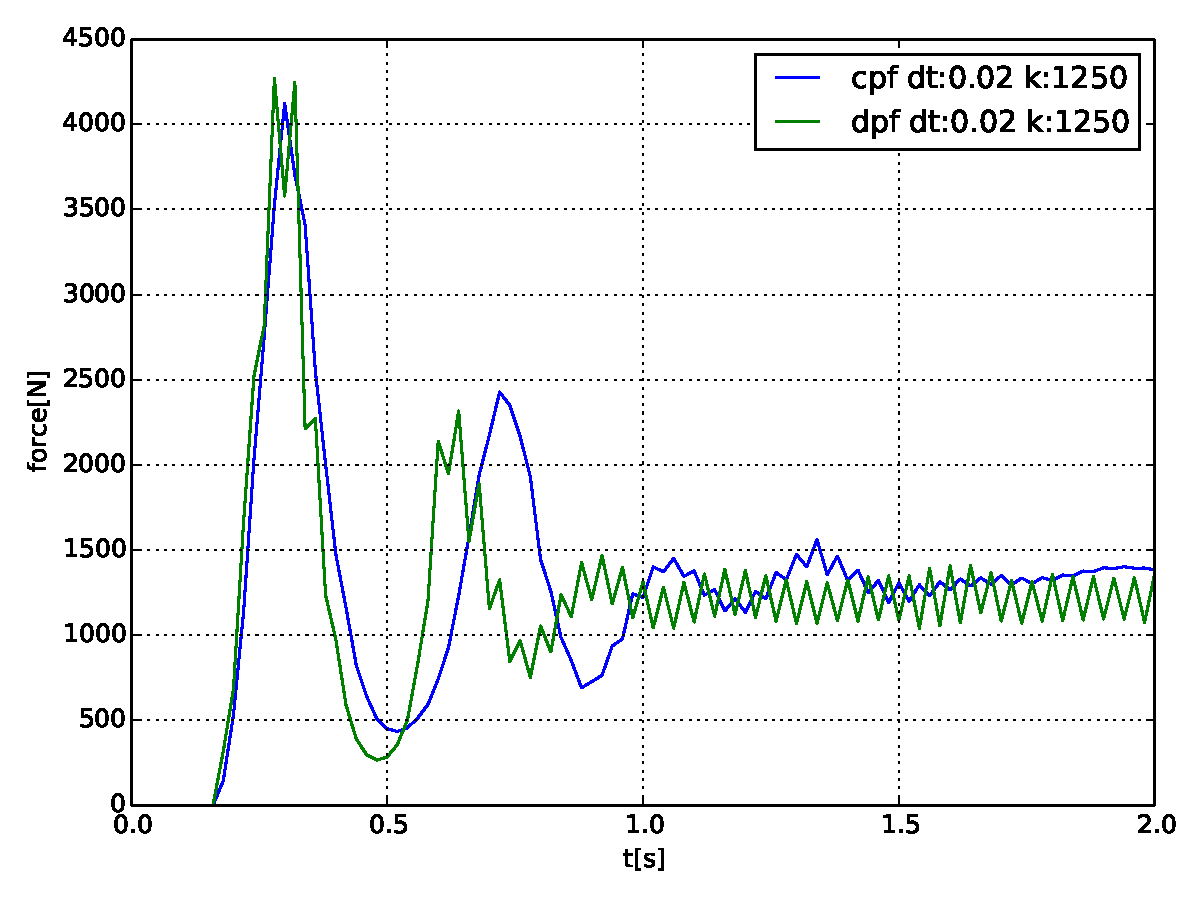
\includegraphics[width=1.0\linewidth]{pics/pdf/cubeBM_t002.pdf} }
		\end{minipage}
		\begin{minipage}[b]{0.5 \linewidth}
			\centering
			\subfigure[$\Delta$t=0.04, k=500]{
				       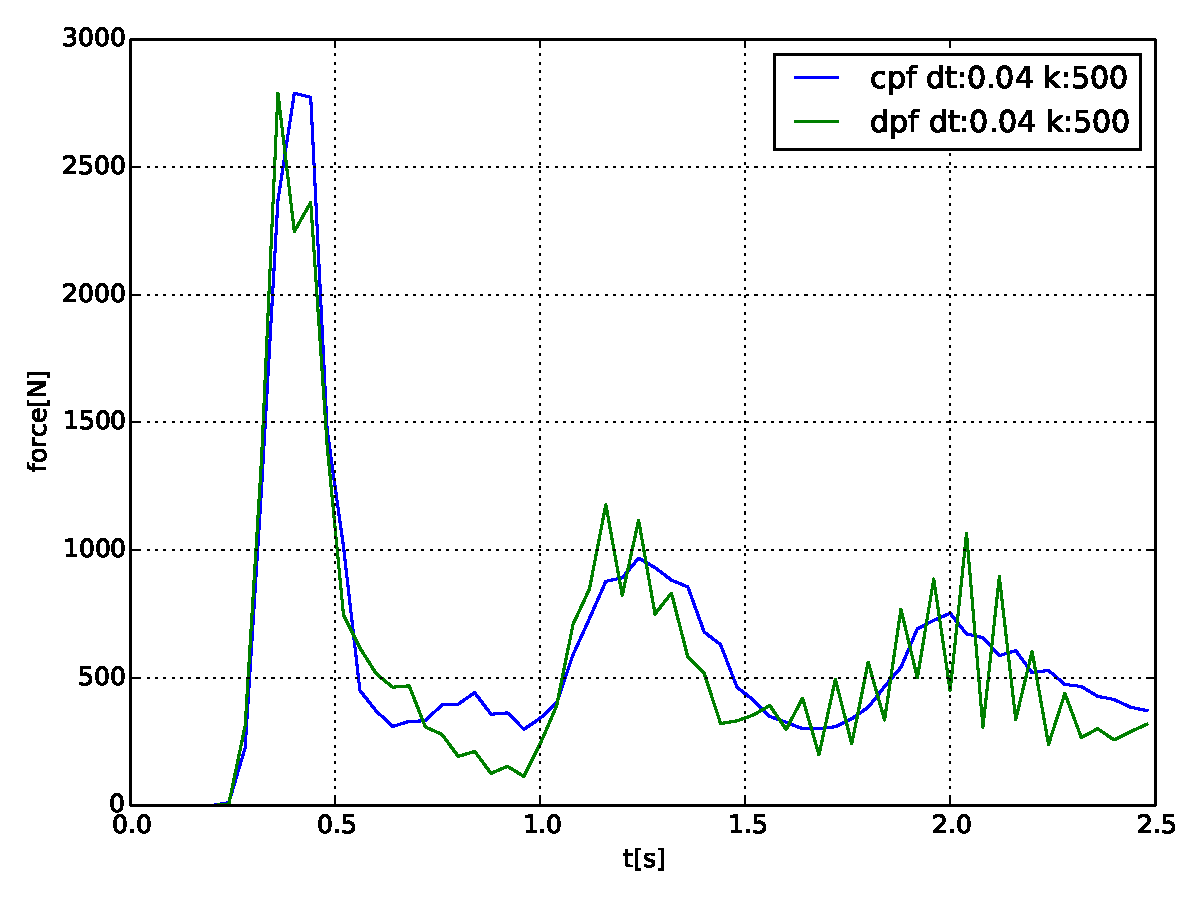
\includegraphics[width=1.0\linewidth]{pics/pdf/cubeBM_t004.pdf} }
		\end{minipage}

  \caption{The repulsion force between a deformable bar and a rigid cube with varying time steps dt and penalty coefficients k.}
  \label{fig::defBar_vs_RigCubeBM}
\end{figure}
\begin{figure}[h] 
		\centering
			       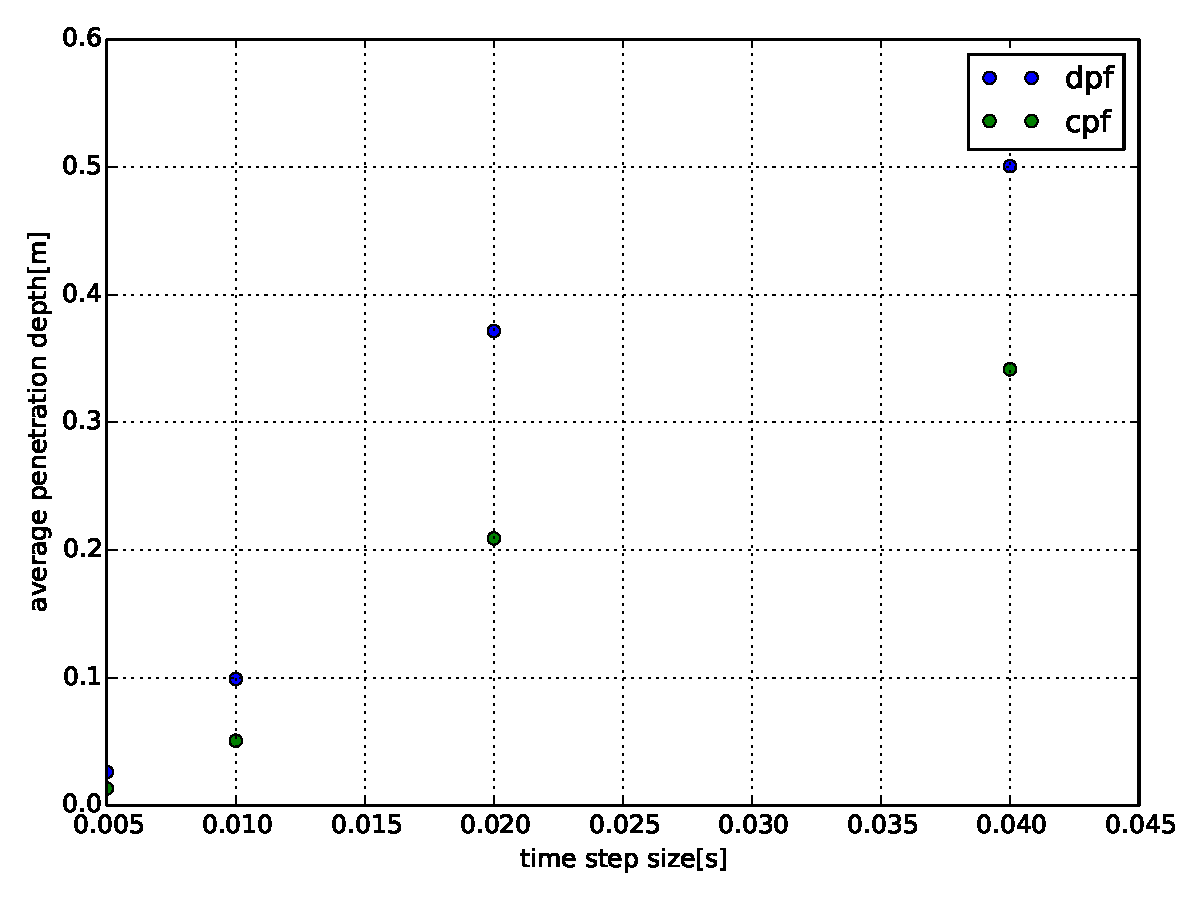
\includegraphics[width=0.5\linewidth]{pics/pdf/defBar_vs_RigCubeBM_depth.pdf} 

  \caption[The average of the summed penetration depth per time step for a deformable bar dropped on a rigid cube with varying time steps an penalty coefficients.]{The average of the summed penetration depth per time step for a deformable bar dropped on a rigid cube with varying time steps and penalty coefficients. For increasing time steps the penalty coefficients decrease and accordingly the penetration depth increases. It is noticeable that the penetration depth with CPF is between 1.4 and 2.0 times higher than the penetration depth with DPF.}
  \label{fig::defBar_vs_RigCubeBM_depth}
\end{figure}
However, the summed penetration depth per time step, as shown in figure \ref{fig::defBar_vs_RigCubeBM_depth}, is for CPF  between 1.4 and 2.0 times larger than for DPF. The DPF algorithm yields larger collison forces due to the larger overestimation of the penetration depth while the intersection is increasing, as explained in section \ref{sec:CPFGENERAL}.

We have shown that the penetration depth for CPF is larger than for DPF with equal penalty coefficients, but for these cases the DPF were already jittering whereas CPF behaved smooth. In order to make a valid statement, we have to investigate the penetration depth and the jitter for varying penalty coefficients.

\begin{figure}[h!] 
\begin{minipage}[b]{0.5 \linewidth}
		\centering
		\subfigure[CPF]{
			       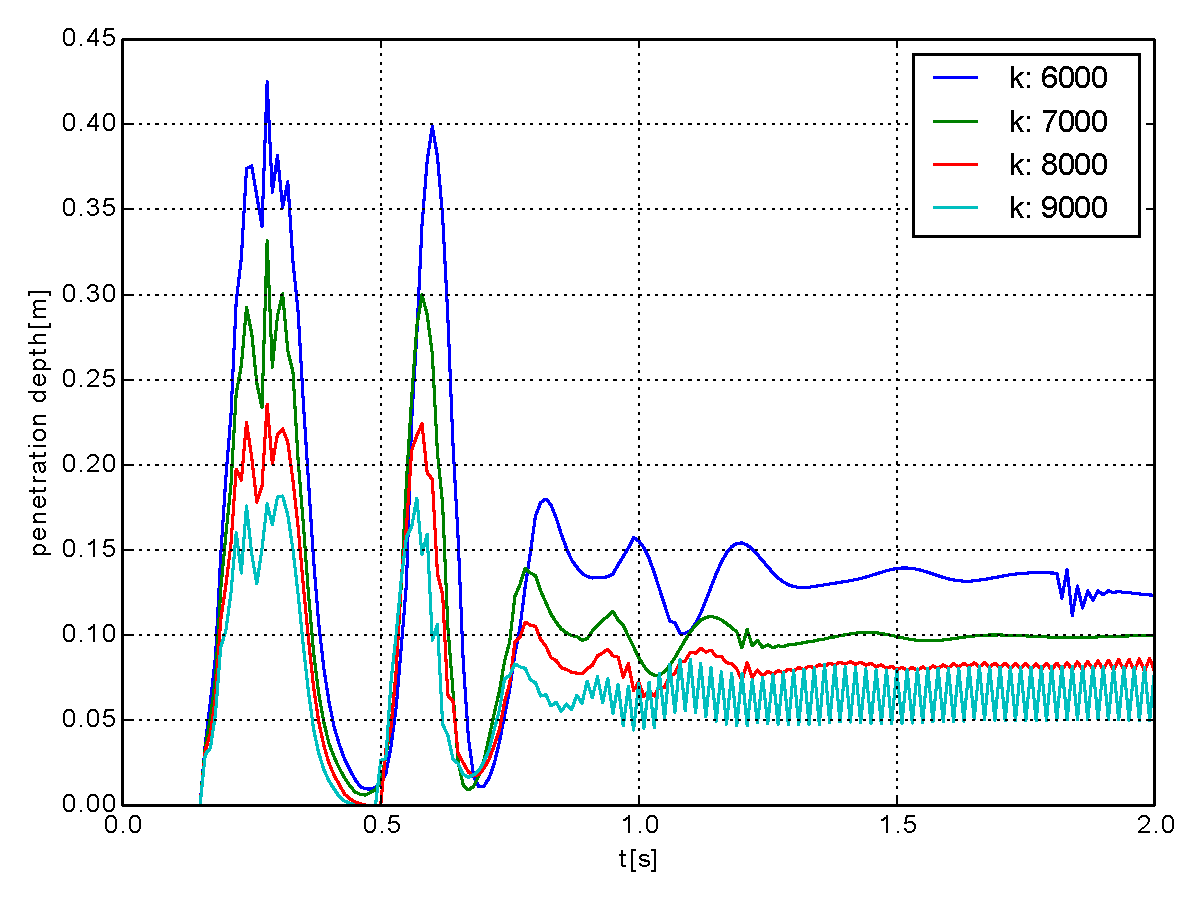
\includegraphics[width=1.0\linewidth]{pics/pdf/pendepth_cpf.pdf} }
	\end{minipage}
	\begin{minipage}[b]{0.5 \linewidth}
		\centering
		\subfigure[DPF]{
			       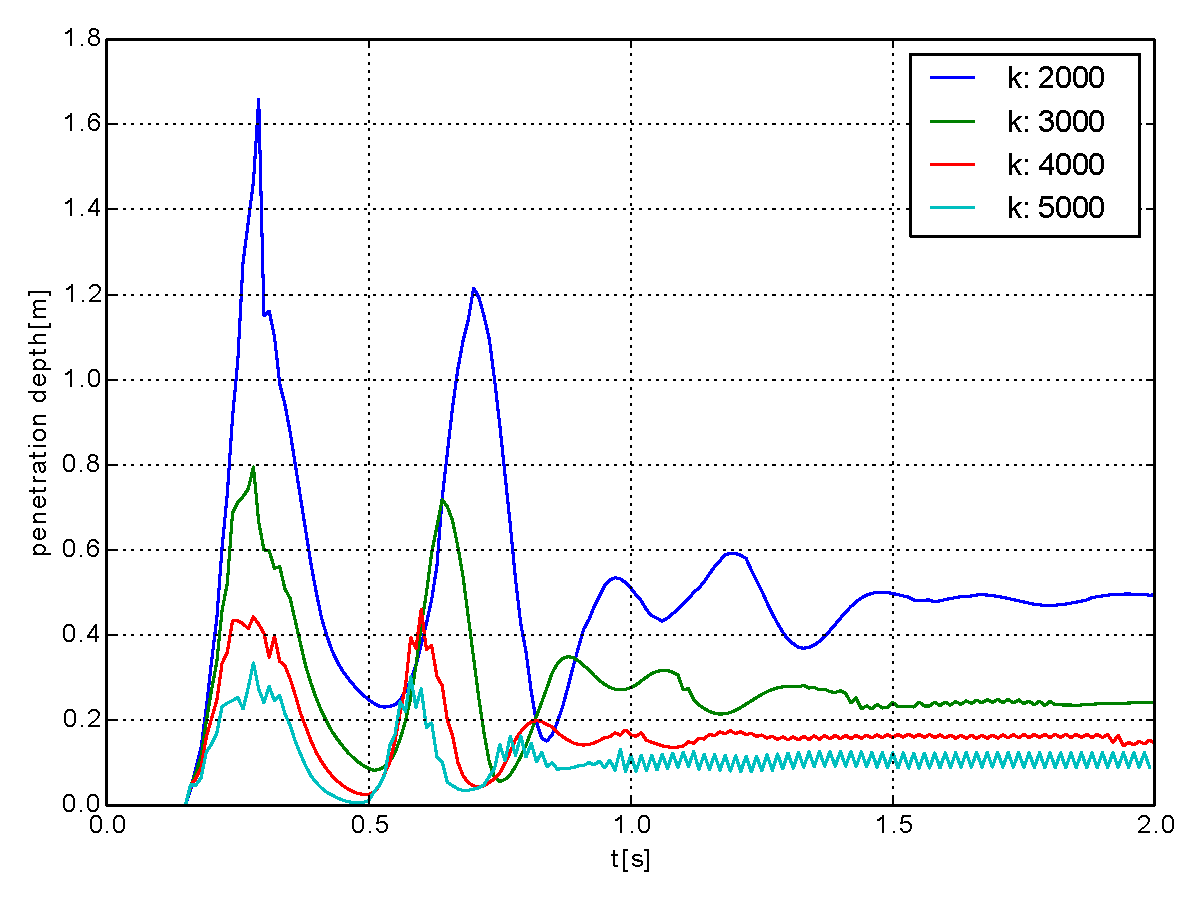
\includegraphics[width=1.0\linewidth]{pics/pdf/pendepth_dpf.pdf} }
	\end{minipage}
  \caption[The penetration depth for CPF and DPF with varying penalty coefficients and constant time step $\Delta t=0.01s$.]{The penetration depth for CPF and DPF with varying penalty coefficients and constant time step $\Delta t=0.01s$. (Note the different scaling of the y-axis and the different penalty coefficients). For the equilibrium, CPF provide smooth behavior up to k=8000 with a penetration depth of 0.1m, whereas DPF only provide an almost smooth behavior up to k=3000, with a penetration depth of 0.28m.}
  \label{fig::pendepth_comp}
\end{figure}

Again, we drop the deformable bar on the rigid cube, this time with a constant time step $\Delta t=0.01$ and varying penalty coefficients $k$. The penetration depths are shown in figure \ref{fig::pendepth_comp}.
For the equilibrium CPF, provide smooth behavior up to k=7000 with a penetration depth of 0.1m, whereas DPF only provide an almost smooth behavior up to $k=3000$, with a penetration depth of 0.28m.



In this section, we compared the CPF algorithm by Tang et al. \cite{TANG2012} to DPF and showed that for a constant penalty coefficient CPF can handle larger time steps without jitter. However, the DPF provide smaller penetration depths with an equal penalty coefficient. Nevertheless, with an increased penalty coefficient for the CPF, CPF are still stable and provide smaller intersections. In comparison, the DPF are with a smaller penalty coefficient already jittering and yield larger penetration depths.

In conclusion the CPF algorithm provides increased stability, less jitter and smaller penetration depths.

\section{Contact Redefinition}
\label{sec::res_redef}
To analyze the new approach of contact redefinition (described in section \ref{sec::CPFExtensions}) we simulate a rigid cube sliding on a deformable bar with and without the collision redefinition algorithm (see figures \ref{fig::redef_collsVFwo}- \ref{fig::redef_collsEE}). There is no friction applied, therefore the tangential motion should not change.

Without the redefinition algorithm the rigid cube changes its velocity in an implausible fashion tangential to the bar and bounces between the surface edges and vertices of the bar. It is hooked between the surface elements. The tangential forces are caused by the highlighted collisions in figure \ref{fig::redef_collsEEwo} (b)-(f) and \ref{fig::redef_collsVFwo} (f). Furthermore, there are implausible collisions in \ref{fig::redef_collsVFwo} (b)and (c). The highlighted vertices  \ref{fig::redef_collsVFwo} (b)and (c) would be expected to be colliding with the vertex of the face directly below and not with the neighboring face.
In contrast, with the redefinition algorithm (see figure  \ref{fig::redef_collsVF} and \ref{fig::redef_collsVF}) the cube's tangential velocity does not change notable, it slides on the bar and tips over the edge. There are no wrong collisions inducing strong tangential forces and no implausible collision pairs.

\begin{figure}[tbp] 
			\begin{minipage}[b]{0.3 \linewidth}
				\centering
				\subfigure[t=0.00s]{
					       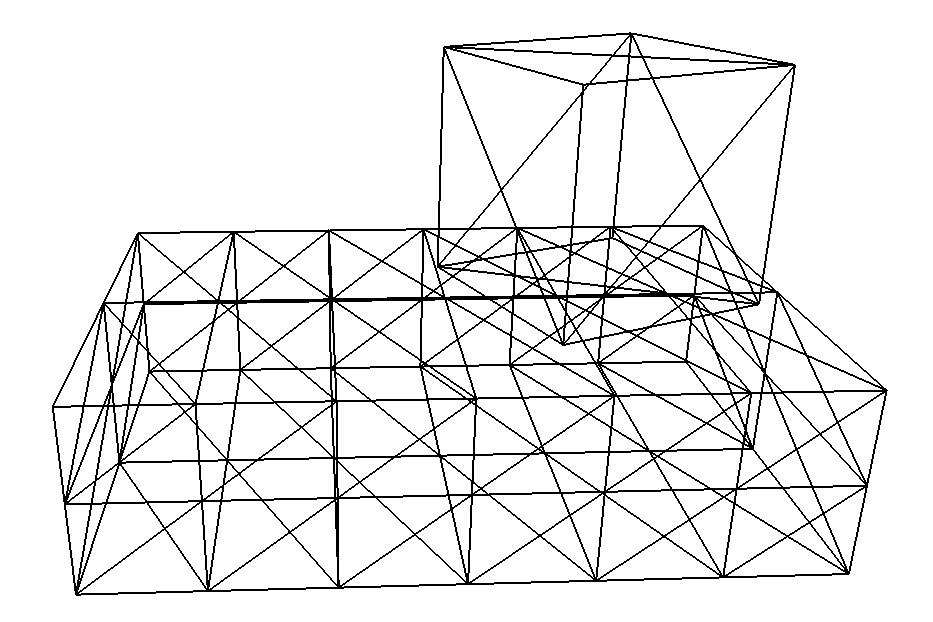
\includegraphics[width=1.0\linewidth]{pics/png/redef_vf01wo.png} }
			\end{minipage}
			\begin{minipage}[b]{0.3 \linewidth}
				\centering
				\subfigure[t=0.50s]{
					       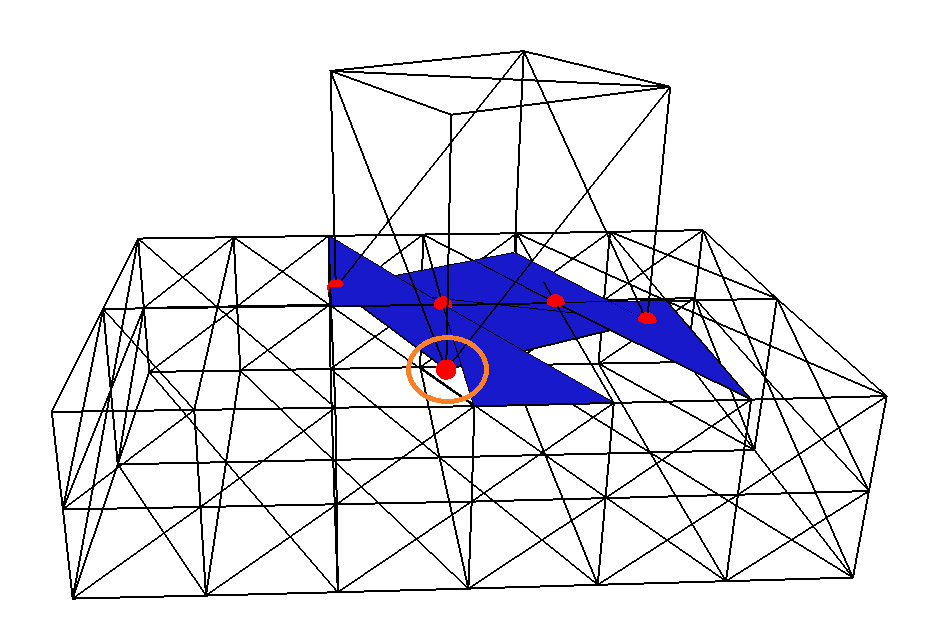
\includegraphics[width=1.0\linewidth]{pics/png/redef_vf02wo.png} }
			\end{minipage}
			\begin{minipage}[b]{0.3 \linewidth}
				\centering
				\subfigure[t=1.00s]{
		       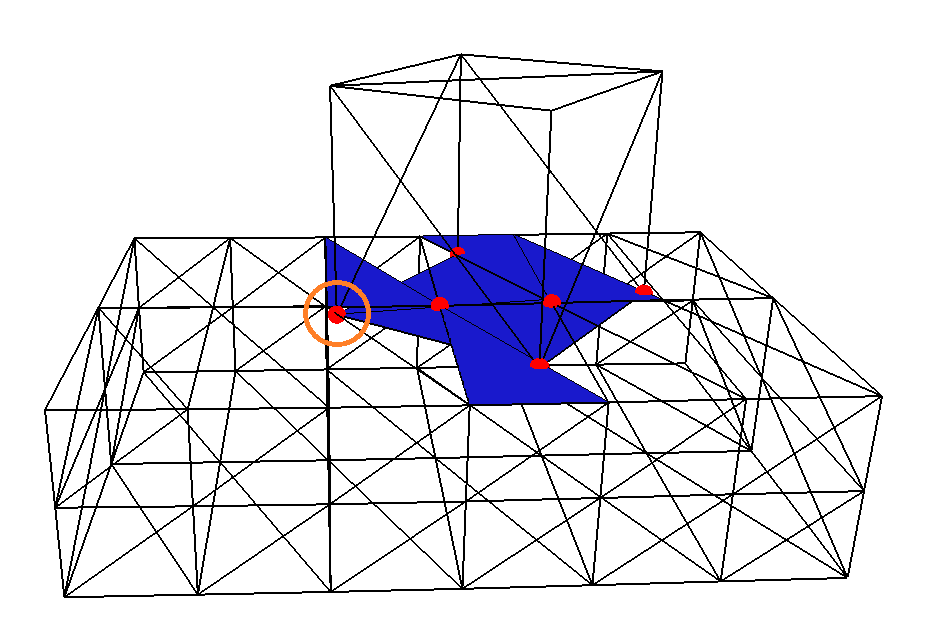
\includegraphics[width=1.0\linewidth]{pics/png/redef_vf03wo.png} }
			\end{minipage}\\
			
				\begin{minipage}[b]{0.3 \linewidth}
					\centering
					\subfigure[t=1.50s]{
						       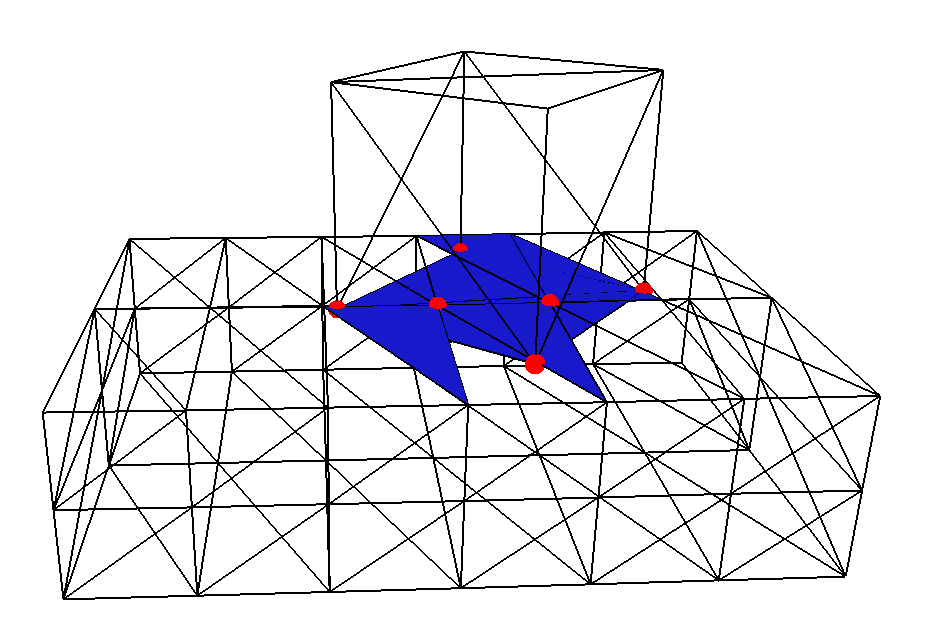
\includegraphics[width=1.0\linewidth]{pics/png/redef_vf04wo.png} }
				\end{minipage}
				\begin{minipage}[b]{0.3 \linewidth}
					\centering
					\subfigure[t=2.00s]{
						       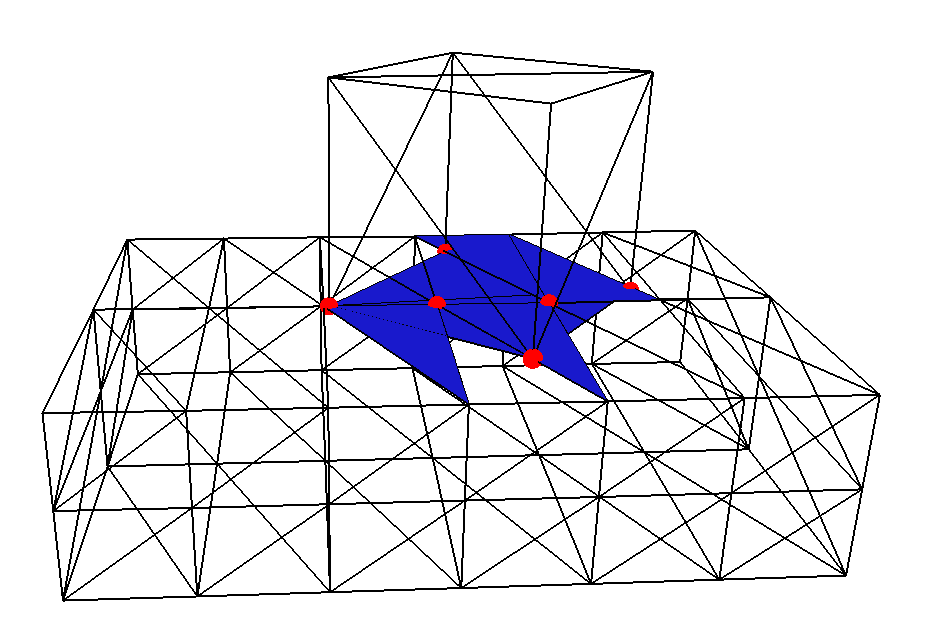
\includegraphics[width=1.0\linewidth]{pics/png/redef_vf05wo.png} }
				\end{minipage}
				\begin{minipage}[b]{0.3 \linewidth}
					\centering
					\subfigure[t=2.50s]{
			       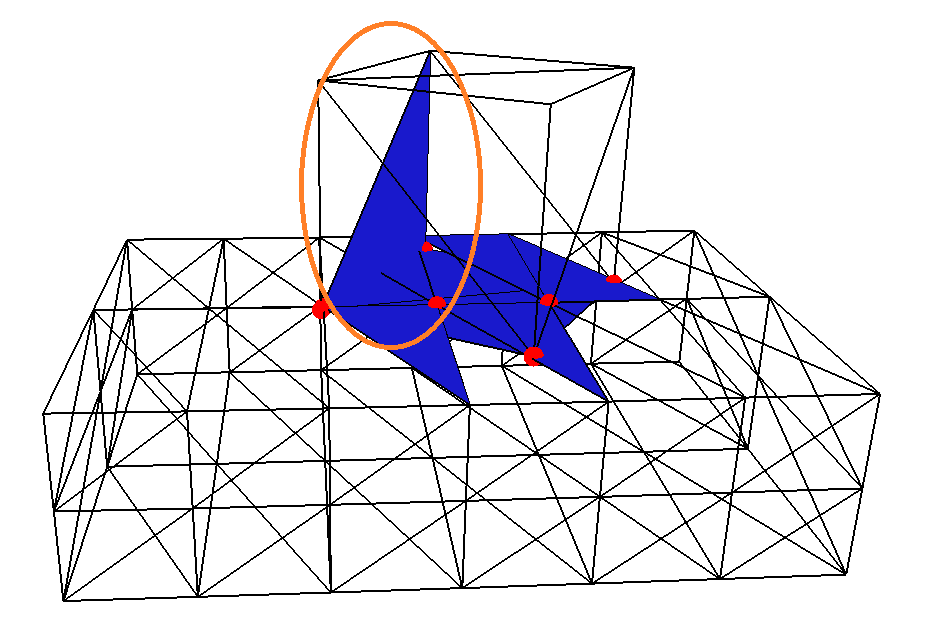
\includegraphics[width=1.0\linewidth]{pics/png/redef_vf06wo.png} }
				\end{minipage}\\
				\caption[A rigid cube sliding on a deformable bar without the collision redefinition algorithm and without friction.]{A rigid cube sliding on a deformable bar without the collision redefinition algorithm and without friction. The sideway collision pairs induce implausible tangential forces affecting the movement of the rigid cube in an implausible way.  The subfigures show active VF collisions, with the vertices in red and the faces in blue, the features inducing artifact forces are highlighted orange.}
				\label{fig::redef_collsVFwo}
\end{figure}

\begin{figure}[tbp] 
			\begin{minipage}[b]{0.3 \linewidth}
				\centering
				\subfigure[t=0.00s]{
					       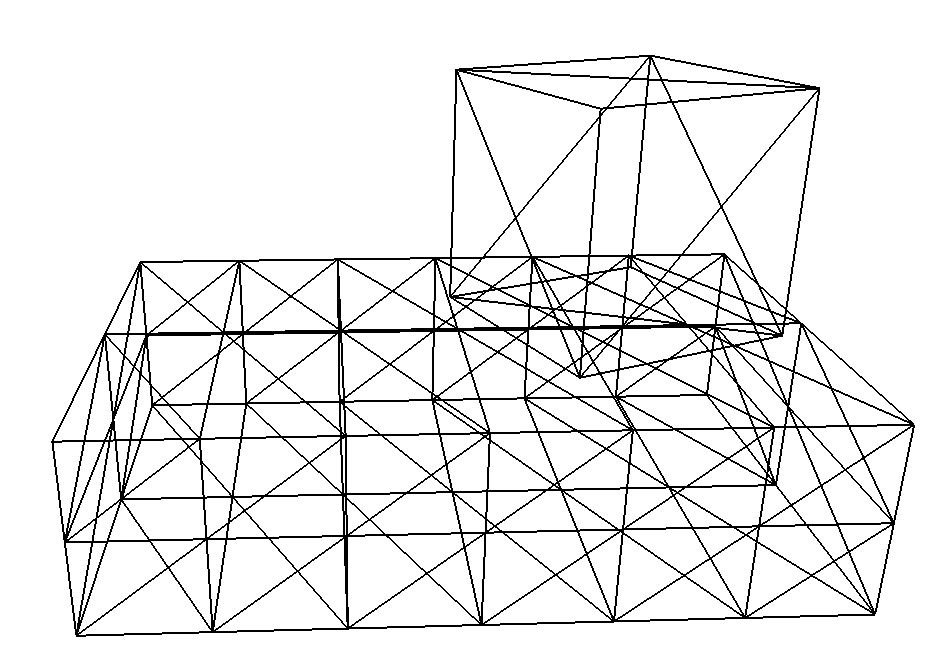
\includegraphics[width=1.0\linewidth]{pics/png/redef_vf01.png} }
			\end{minipage}
			\begin{minipage}[b]{0.3 \linewidth}
				\centering
				\subfigure[t=0.50s]{
					       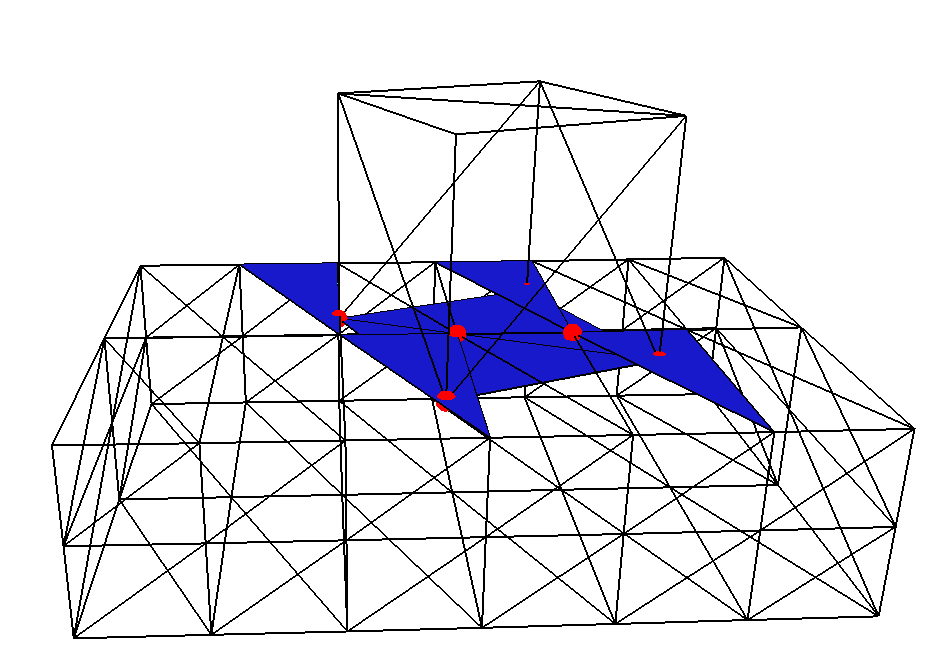
\includegraphics[width=1.0\linewidth]{pics/png/redef_vf02.png} }
			\end{minipage}
			\begin{minipage}[b]{0.3 \linewidth}
				\centering
				\subfigure[t=1.00s]{
		       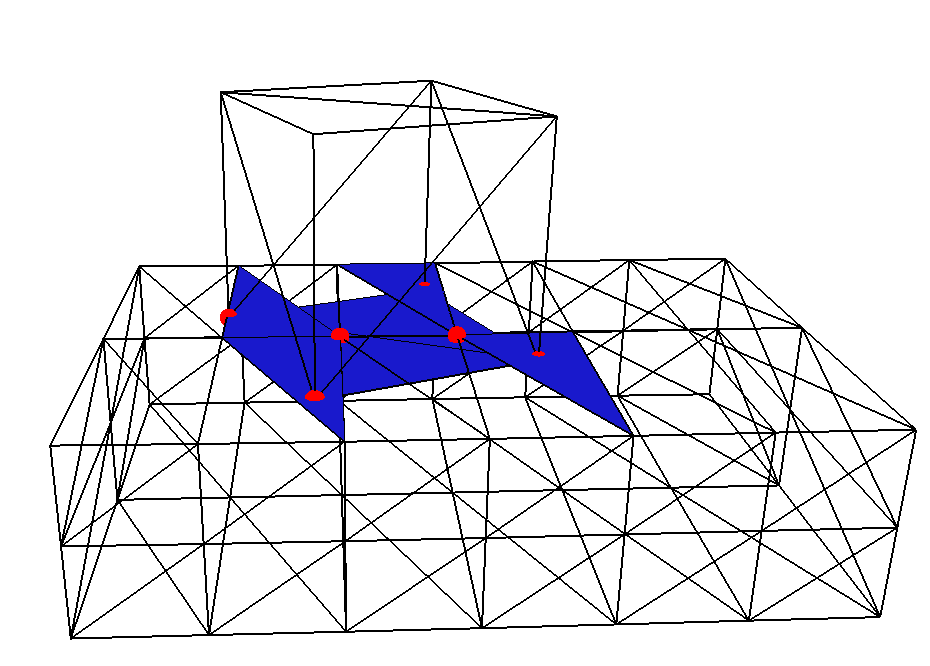
\includegraphics[width=1.0\linewidth]{pics/png/redef_vf03.png} }
			\end{minipage}\\
			
				\begin{minipage}[b]{0.3 \linewidth}
					\centering
					\subfigure[t=1.50s]{
						       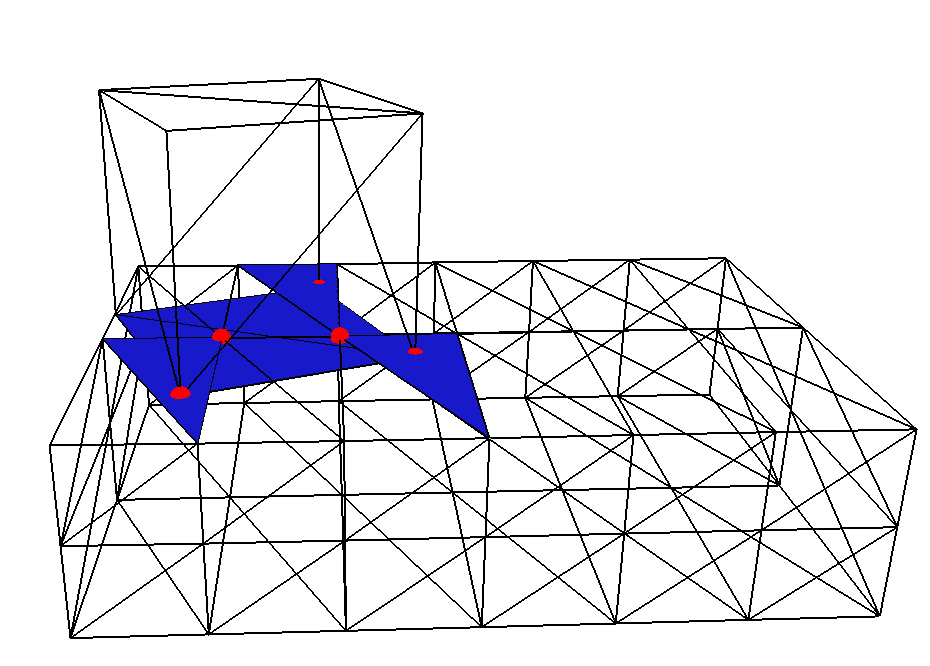
\includegraphics[width=1.0\linewidth]{pics/png/redef_vf04.png} }
				\end{minipage}
				\begin{minipage}[b]{0.3 \linewidth}
					\centering
					\subfigure[t=2.00s]{
						       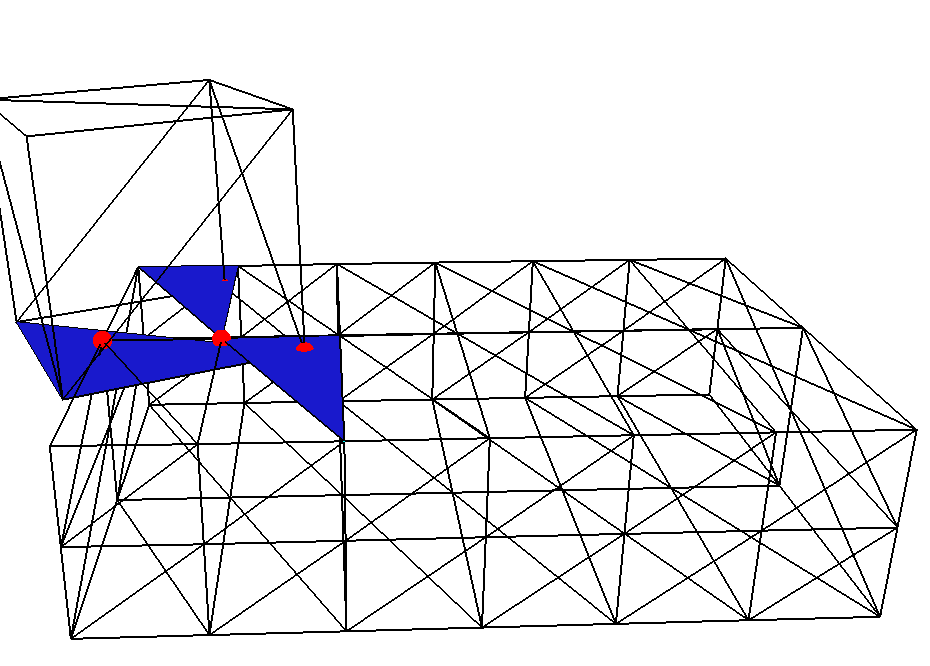
\includegraphics[width=1.0\linewidth]{pics/png/redef_vf05.png} }
				\end{minipage}
				\begin{minipage}[b]{0.3 \linewidth}
					\centering
					\subfigure[t=2.50s]{
			       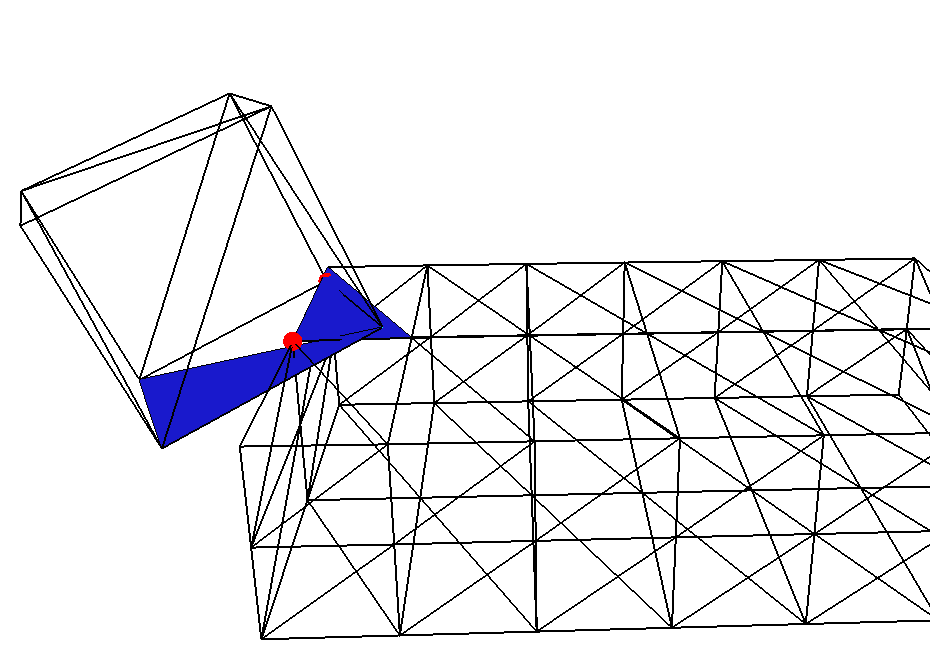
\includegraphics[width=1.0\linewidth]{pics/png/redef_vf06.png} }
				\end{minipage}\\
				\caption[A rigid cube sliding on a deformable bar with the collision redefinition algorithm and without friction.]{A rigid cube sliding on a deformable ba with the collision redefinition algorithm and without friction. With the redefinition algorithm no sideways collision appear and the cube slides plausible on the bar without notable changes in its tangential velocity. The subfigures show active VF collisions, with the vertices in red and the faces in blue.}
				\label{fig::redef_collsVF}
\end{figure}

\begin{figure}[tbp] 
	\begin{minipage}[b]{0.3 \linewidth}
		\centering
		\subfigure[t=0.00s]{
			       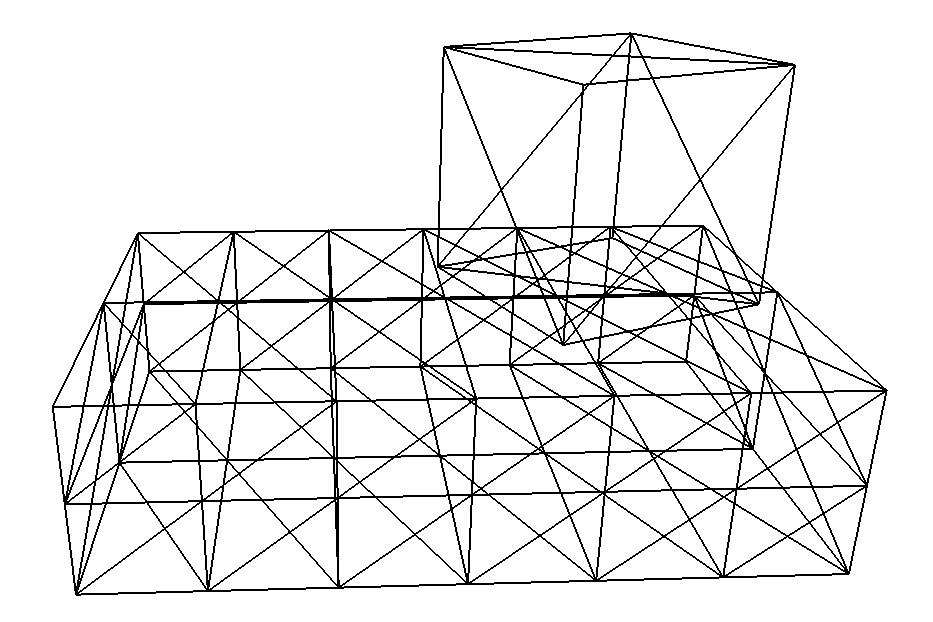
\includegraphics[width=1.0\linewidth]{pics/png/redef_ee01wo.png} }
	\end{minipage}
	\begin{minipage}[b]{0.3 \linewidth}
		\centering
		\subfigure[t=0.50s]{
			       \includegraphics[width=1.0\linewidth]{pics/png/redef_ee02wo.png} }
	\end{minipage}
	\begin{minipage}[b]{0.3 \linewidth}
		\centering
		\subfigure[t=1.00s]{
       \includegraphics[width=1.0\linewidth]{pics/png/redef_ee03wo.png} }
	\end{minipage}\\
	
		\begin{minipage}[b]{0.3 \linewidth}
			\centering
			\subfigure[t=1.50s]{
				       \includegraphics[width=1.0\linewidth]{pics/png/redef_ee04wo.png} }
		\end{minipage}
		\begin{minipage}[b]{0.3 \linewidth}
			\centering
			\subfigure[t=2.00s]{
				       \includegraphics[width=1.0\linewidth]{pics/png/redef_ee05wo.png} }
		\end{minipage}
		\begin{minipage}[b]{0.3 \linewidth}
			\centering
			\subfigure[t=2.50s]{
	       \includegraphics[width=1.0\linewidth]{pics/png/redef_ee06wo.png} }
		\end{minipage}
				\caption[A rigid cube sliding on a deformable bar without the collision redefinition algorithm and without friction.]{A rigid cube sliding on a deformable bar without the collision redefinition algorithm and without friction. The sideway collision pairs induce implausible tangential forces affecting the movement of the rigid cube in an implausible way. The subfigures show EE collisions in green and the collisions inducing implausible tangential forces are highlighted orange.}
				\label{fig::redef_collsEEwo}
\end{figure}

\begin{figure}[tbp] 
	\begin{minipage}[b]{0.3 \linewidth}
		\centering
		\subfigure[t=0.00s]{
			       \includegraphics[width=1.0\linewidth]{pics/png/redef_ee01.png} }
	\end{minipage}
	\begin{minipage}[b]{0.3 \linewidth}
		\centering
		\subfigure[t=0.50s]{
			       \includegraphics[width=1.0\linewidth]{pics/png/redef_ee02.png} }
	\end{minipage}
	\begin{minipage}[b]{0.3 \linewidth}
		\centering
		\subfigure[t=1.00s]{
       \includegraphics[width=1.0\linewidth]{pics/png/redef_ee03.png} }
	\end{minipage}\\
	
		\begin{minipage}[b]{0.3 \linewidth}
			\centering
			\subfigure[t=1.50s]{
				       \includegraphics[width=1.0\linewidth]{pics/png/redef_ee04.png} }
		\end{minipage}
		\begin{minipage}[b]{0.3 \linewidth}
			\centering
			\subfigure[t=2.00s]{
				       \includegraphics[width=1.0\linewidth]{pics/png/redef_ee05.png} }
		\end{minipage}
		\begin{minipage}[b]{0.3 \linewidth}
			\centering
			\subfigure[t=2.50s]{
	       \includegraphics[width=1.0\linewidth]{pics/png/redef_ee06.png} }
		\end{minipage}
				\caption[A rigid cube sliding on a deformable barwith the collision redefinition algorithm and without friction.]{A rigid cube sliding on a deformable bar with the collision redefinition algorithm and without friction. With the redefinition algorithm no sideways collision appear and the cube slides plausible on the bar without notable changes in its tangential velocity. The subfigures show active EE collisions in green and candidate collisions in red.}
				\label{fig::redef_collsEE}
\end{figure}

The repulsion forces are shown in figure \ref{fig::force_redef}. The plot shows a smooth with several leaps. The leaps are induced by the contact redefinitions. When a sliding contact is redefined, there is a sudden additional geometrically deep collision providing a sudden increase of the contact force. Similarly, if an EE collision is added or removed by the redefinition algorithm, force changes are induced. Overall, these leaps are small and do not induce a notable jitter.

\begin{figure}[tbp]
\centering
\includegraphics[width=0.60\linewidth]{pics/pdf/slidingCube_redef_dt.pdf} 
\caption{Contact force for a rigid cube sliding on a deformable bar}
\label{fig::force_redef}
\end{figure}
\begin{figure}[tbp] 
	\begin{minipage}[b]{0.33 \linewidth}
		\centering
		\subfigure[t=0.00s]{
			       \includegraphics[width=0.97\linewidth]{pics/png/bunny01.png} }
	\end{minipage}
	\begin{minipage}[b]{0.33 \linewidth}
		\centering
		\subfigure[t=0.50s]{
			       \includegraphics[width=0.97\linewidth]{pics/png/bunny02.png} }
	\end{minipage}
	\begin{minipage}[b]{0.33 \linewidth}
		\centering
		\subfigure[t=1.00s]{
       \includegraphics[width=0.97\linewidth]{pics/png/bunny03.png} }
	\end{minipage}\\
	
		\begin{minipage}[b]{0.33 \linewidth}
			\centering
			\subfigure[t=1.50s]{
				       \includegraphics[width=0.97\linewidth]{pics/png/bunny04.png} }
		\end{minipage}
		\begin{minipage}[b]{0.33 \linewidth}
			\centering
			\subfigure[t=2.00s]{
				       \includegraphics[width=0.97\linewidth]{pics/png/bunny05.png} }
		\end{minipage}
		\begin{minipage}[b]{0.33 \linewidth}
			\centering
			\subfigure[t=2.50s]{
	       \includegraphics[width=0.97\linewidth]{pics/png/bunny06.png} }
		\end{minipage}
				\caption{A deformable bunny is dropped in a rigid bowl, which is dropped on a static plane.}
				\label{fig::bunnyBowl}
\end{figure}

\begin{figure}[tbp]
		\centering
			       \includegraphics[width=0.4\linewidth]{pics/png/bunny_inverted.png} 
	
\caption{Inverted tetrahedrons (marked red) occur when the deformable bunny collides with the rigid bowl.}
\label{fig::bunny_inverted}
\end{figure}

Up to now we analyzed rather simple geometries. Therefore, we will now investigate a more complex scene, with a bunny dropped in a rigid bowl with CPF and the redefinition algorithm. Screenshots of the simulation are shown in figure \ref{fig::bunnyBowl}.

The bunny drops in the bowl, bounces around for approximately two seconds and then comes to rest. The overall result is visually satisfying. However, a closer look at the bunny shows that when it is colliding some tetrahedrons are inverted , see figure \ref{fig::bunny_inverted}. Inverted tetrahedrons disturb the visual impression of the scene. They are induced due to large collision impulses by the CPF algorithm and can be reduced by choosing lower penalty coefficients. Nevertheless, reducing the penalty coefficients yields larger penetration depths.
\newpage

To sum it up, we have shown in the cube-bar benchmark that the redefinition algorithm provides plausible collision pairs and preserves the tangential motion, whereas with the original CPF algorithm we obtained an implausible stop of the tangential motion. Furthermore, we proved that the redefinition algorithm can handle complex geometries, as shown in the bunny-bowl scene.

\section{Friction}
To achieve a plausible friction behavior, the friction model should induce forces according to Coulombs law. Dynamic friction should slow down the tangential movement. Static friction should stop any tangential movement if the tangential velocity is close to zero and the tangential force $\mathbf f_t$ is smaller than the product of the static friction coefficient $\mu_S $ and the normal force $\mathbf f_n$.


To analyze the friction model, we investigate a rigid cube with mass $m=100kg$ sliding on a $10^\circ$ slope. To test the static friction, the velocity of the rigid cube is initialized with $v_0=3\frac{m}{s}$ upwards the plane. We used continuous penalty forces with a penalty coefficient $k=20000$. The dynamic friction coefficient is set to $\mu_d=0.1$ and the static friction is set to $\mu_s=0.3$ and $\mu_s=0.4$. The friction penalty coefficients are set to $k_{fp}=100$, $k_{fd}=25$ and $k_f=10000$.

\begin{figure}[h!]
	\begin{minipage}[b]{0.5 \linewidth}
		\centering
		\subfigure[static friction coefficients $\mu_s=0.3$]{
			       \includegraphics[width=1.0\linewidth]{pics/pdf/block_fric_dyn.pdf} }
	\end{minipage}
	\begin{minipage}[b]{0.5 \linewidth}
		\centering
		\subfigure[static friction coefficients $\mu_s=0.4$]{
			       \includegraphics[width=1.0\linewidth]{pics/pdf/block_fric_stat.pdf} }
	\end{minipage}	
\caption[Position and velocity over time of a rigid cube sliding on a slope with different static friction coefficients $\mu_s$.]{Position and velocity over time of a rigid cube sliding on a slope with different static friction coefficients $\mu_s$. With the lower coefficient $\mu_s=0.3$ the cube slides up the slope until its velocity reaches zero, then it starts sliding down. Whereas, with the higher coefficient $\mu_s$ the cube stops after its velocity reached zero and stays at its position.}
\label{fig::friction_dynstat}
\end{figure}

The movement and the velocity of the cube are shown in figure \ref{fig::friction_dynstat}.
For the lower coefficient $\mu_s=0.3$ the cube slides up the plane with decreasing velocity, decelerated by gravity and dynamic friction.
At $t\approx 1.2s$ it reaches the maximum height and starts sliding down again with increasing velocity, this time accelerated by gravity and slightly decelerated by dynamic friction.

For the higher coefficient $\mu_s=0.4$ the cube starts exactly equal to the previous one. However, when it reaches the top it remains at the position, due to the increased static friction coefficient. The static friction is now larger than the	downhill-slope force. The velocity shows a small damped oscillation at $t\approx 1.2s$, it is induced since we model the static friction by applying a damped spring at the point where the cube is to be hold.

Comparing the results with the analytical solution of Coulomb's Friction law, we would expect the block to stop for $\mu_s>0.176$, whereas in our simulation the block stopped for $\mu_s \gtrsim 0.4$. Nevertheless the friction model provides  results analogously to Coulomb's Friction law, providing satisfying results for an interactive environment.

To analyze the friction between multiple bodies we place a rigid cube with an initial velocity on a deformable bar and simulate two different friction coefficients. Furthermore, to test for numerical drift in the position due to the static friction we will analyze the simulation for a large number of time steps (20000).

\begin{figure}[h!]
	\begin{minipage}[b]{0.5 \linewidth}
		\centering
		\subfigure[$\mu_s=0.8$, $\mu_d=0.1$, $t=0.2s$]{
			       \includegraphics[width=1.0\linewidth]{pics/png/sliding_block_mus08_md01_a.png} }
	\end{minipage}
	\begin{minipage}[b]{0.5 \linewidth}
		\centering
		\subfigure[$\mu_s=0.8$, $\mu_d=0.1$, $t=20.0s$]{
			       \includegraphics[width=1.0\linewidth]{pics/png/sliding_block_mus08_md01_b.png} }
	\end{minipage}\\
	
		\begin{minipage}[b]{0.5 \linewidth}
			\centering
			\subfigure[$\mu_s=0.3$, $\mu_d=0.05$, $t=0.35s$]{
				       \includegraphics[width=1.0\linewidth]{pics/png/sliding_block_mus03_md005_a.png} }
		\end{minipage}
		\begin{minipage}[b]{0.5 \linewidth}
			\centering
			\subfigure[$\mu_s=0.3$, $\mu_d=0.05$, $t=20.0s$]{
				       \includegraphics[width=1.0\linewidth]{pics/png/sliding_block_mus03_md005_b.png} }
		\end{minipage}		
\caption[A rigid cube sliding from the right to the left on a deformable bar with two friction coefficient combinations.]{A rigid cube sliding from the right to the left on a deformable bar with two friction coefficient combinations. (a) and (c) show the cube right after the static friction set in. (b) and (d) show the cube after two seconds. With the lower valued coefficient combination the cube keeps sliding further than with higher combination due to dynamic friction. After the blocks stopped they rest at their position due to static friction.}
\label{fig::block_sliding_fric_longtime}
\end{figure}

Screenshots of the scene are shown in figure \ref{fig::block_sliding_fric_longtime}. The cube starts at the right side with its initial velocity in the left direction. With the higher friction coefficients in a) and b) the cube is stronger decelerated as with the lower coefficients in c) and d).
After the cube stopped it movements (a) and c), it rests exactly at its position. Even after 20000 steps there is no numerical drift in the position notable. This a result of the static friction modeled with a fixed spring. Therefore the bodies can make small movements around the fixed position, but no optically notable movement or position drift is possible.

In conclusion the penalty-based friction model \cite{YAMANE2006} applies a plausible modeling of dynamic and static friction with no notable numerical drift in the position for the static friction.
The model does not grant the analytical description of Coulomb's friction law. However it provides analogue results, which are satisfying for the use in an interactive environment.


\section{Computational Cost}
\label{sec:compCost}
The computational cost is a crucial property for interactive applications. Therefore, we investigate the computational cost of the CPF in comparison to the DPF with regard to the results from the stability analysis.
 
We analyzed the scene with a deformable bunny dropped into a rigid bowl from section \ref{sec::res_redef} (see figure \ref{fig::bunnyBowl}) using an Intel Core i7-2630QM 2.0Ghz processor with 6.0GB RAM and a Nvidia Geforce 540M graphics card.
To provide an accurate comparison of the CPF and DPF, we simulate the scene with CPF and compute for each feature pair the impulse with both algorithms, though DPF computation is only for time measurements and the impulses are not applied.
We measured five runs with 200 simulation steps each and detecting the time for the handling of each feature and its components.
The averaged times are shown in figure \ref{fig::compCost_scene}.

\begin{figure}[h]
		\centering
			       \includegraphics[width=0.9\linewidth]{pics/pdf/comparison_comptime_cpf_dpf.pdf} 	
\caption{Composition of the computation time for one feature pair}
\label{fig::compCost_scene}
\end{figure}
The handling for a single EE pair takes average $6.8\mu s$, whereas a VF pair is slightly slower and takes average $7.8 \mu s$. The difference is mainly caused by the overall most expensive part of the collision handling, the categorization of the collision. For the EE pair, the collision categorization takes average $3.11 \mu s$ and thereby $45.7\%$ of the overall time for one feature pair. In the VF case, the categorization takes average $4.07\mu s$ and thereby $53.1 \%$ of the overall time for one feature pair.
The difference in the computation time of the VF and EE categorization can be explained by examining the number of tested normals. 
A vertex is typically adjacent to six faces and accordingly six normals need to be tested. Whereas, in the EE categorization each edge has only two directly adjacent faces, yielding only four normals to be tested. In sum, there are to more tests for the VF case and consequently the VF categorization is more expensive.
All other parts take almost the same time for VF and EE.
It is remarkable that the actual impulse computation in the VF case with CPF takes only  $12.9 \%$ (EE $14.6\%$) of the overall computation time and for DPF only $3.7\%$ (EE $4.1\%$).


A comparison of the computation time for one impulse with CPF and DPF is shown in figure \ref{fig::comparison_comptime_cpf_dpf_imp}.
The computation of the impulse with CPF takes in the VF case $1,01 \mu s$ (EE $1.00 \mu s$) and for DPF in the VF case it takes $0,29 \mu s$ (EE $0.28 \mu s$). Hence, the DPF need only a third of the time the CPF need for the computation of one impulse. The computational overhead of the CPF seems reasonable, since the CPF require the computation of degree-six polynomial, whereas the DPF correspond to a linear polynomial.
\begin{figure}[tbp]
		\centering
			       \includegraphics[width=0.9\linewidth]{pics/pdf/comparison_comptime_cpf_dpf_imp.pdf} 
	
\caption{Comparison of the computation time for one impulse with CPF and DPF}
\label{fig::comparison_comptime_cpf_dpf_imp}
\end{figure}
However, the impulse computation is only one component in the handling of a collision. In order gain a valid statement, we need to compare the overall computation time for a feature with DPF and CPF. With DPF the handling of one feature pair takes $6.83 \mu s$ (EE $5.84 \mu s$), whereas it takes $7.55 \mu s$ (EE $6.56 \mu s$) with CPF. The handling with CPF takes $11.8\%$ longer than the handling with DPF.
In section \ref{sec::stability} we have shown that the maximum time step for CPF is 1.22 times larger than for DPF. Combining the computational overhead with increased step size yields a theoretical speed-up of $9.12 \%$ for CPF. However, this result provides only limited validity, since DPF require only a DCD, whereas CPF require a CCD. In general, CCD provides a higher computational cost than DCD.

To compare the computational cost of DPF with a state of the art DCD to the computational cost of CPF with a state of the art CCD would yield an interesting and meaningful result in order to evaluate the actual difference in computational cost. However, the CCD in our framework is in a prototype state and far from optimal speed. Therefore, we cannot provide this analysis. However, Tang et al. \cite{TANG2012} compared DPF+DCD to CPF+CCD and showed that CPF+CCD are about 3 - 4 times slower than DPF+DCD.

In conclusion, the redefinition algorithm provides a significant additional cost by almost doubling the time needed to handle one collision pair. However, the additional cost is necessary in order to reduce the CPF artifacts, since otherwise no simulation of sliding contacts is feasible. The additional cost induced by the CPF in comparison to the DPF is small ($+11,8 \%$). However, CPF require CCD. Taking the collision detection into account and comparing the CCD+CPF to DCD+DPF shows that CPF+CCD are about 3 - 4 times slower than DPF+DCD \cite{TANG2012}.
\chapter{Conclusion}

\bibliographystyle{abbrvnat}

\bibliography{bibliography}
		
		% Setzen des Seitenzählers auf den zuvor gespeicherten römischen Seitenzählers und Umstellung auf römische Seitenzahlen
			\pagenumbering{Roman}					%Aktivierung römischer Seitenzahlen
			\setcounter{page}{\value{savecounter}}		%Aufruf der zuvor gespeicherten zuletzt verwendeten römischen Seitenzahl
		% Literaturverzeichnis einfügen
		   % \nocite{*}
			\printbibliography
		% Abbildungsverzeichnis einfügen
			\listoffigures
		% Tabellenverzeichnis einfügen
			\listoftables
		%Abkürzungsverzeichnis einfügen
			
			\glsaddall
			\setlength{\glsdescwidth}{14cm}
			\printglossary[type=\acronymtype,style=long, title=Abkürzungsverzeichnis]
		%Alternatives Abkürzungsverzeichnis einfügen
		%	\chapter*{Abkürzungsverzeichnis}
\addcontentsline{toc}{chapter}{Abkürzungsverzeichnis (tabellarische Alternative)}
\begin{spacing}{1.5}
\setlength\LTleft{15pt}
\setlength\LTright{\fill}
\begin{longtable}{ll}
    \textbf{Abkürzung}	&\textbf{Bedeutung}	\\\midrule\endhead
    TUD	&Technische Universität Darmstadt	\\
    SPZ &Sprachenzentrum	\\
    PMV &Fachgebiet Papierfabrikation und Mechanische Verfahrenstechnik	\\
\end{longtable}
\end{spacing}

                    
		%Symbolverzeichnis einfügen
			\glsaddall
			\setlength{\glsdescwidth}{12.5cm}
			\printglossary[type=symbolslist,style=longheader, title=Symbolverzeichnis]
		%Alternatives Symbolverzeichnis einfügen
		%	\chapter*{Symbolverzeichnis}
\addcontentsline{toc}{chapter}{Symbolverzeichnis (tabellarische Alternative)}
\begin{spacing}{1.5}
\setlength\LTleft{15pt}
\setlength\LTright{\fill}
\begin{longtable}{@{\extracolsep{\fill}}lll}
    \textbf{Symbol}	&\textbf{Einheit}		&\textbf{Beschreibung}                                           \\\midrule\endhead
    \(D\)			&\si{\mm}				&Durchmesser                                                        \\
    \(D_0\)			&\si{\mm}                                           &Ausgangsdurchmesser                                                        \\
    \(\varepsilon\)                &                                           &Dehnung                                                        \\
    \(E\)                &\si{\N\per\mm\squared}                                           &Elastizitätsmodul                                                        \\
    \(G\)                &\si{\N\per\mm\squared}                                           &Schubmodul                                                        \\
    \(\lambda\)                &\si{\nm}                                           &Wellenlänge                                                        \\
    \(l\)                &\si{\mm}                                           &Länge                                                      \\
    \(l_0\)                &\si{\mm}                                           &Ausgangslänge                                                        \\
    \(\Delta l\)                &\si{\mm}                                           &Längendifferenz                                                        \\
    \(n\)                &                                           &Anzahl der Versuche                                                        \\
    \(\omega\)                &\si{\per\s}                                           &Kreisfrequenz                                                        \\
    \(\sigma\)                &\si{\N\per\mm\squared}                                           &Spannung                                                                                                           \\
    \(t\)                &\si{\s}                                           &Zeit                                                        \\
    \(t_0\)                &\si{\s}                                           &Ausgangszeitpunkt                                                        \\
    \(\Delta t\)                &\si{\s}                                           &Zeitdifferenz                                                        \\
    \(T\)                &\si{\degreeCelsius}                                           &Temperatur                                                        \\
    \(T_0\)                &\si{\degreeCelsius}                                           &Ausgangstemperatur bzw. Bezugstemperatur                                                        \\
    \(\Delta T\)                &\si{\degreeCelsius}                                         &Temperaturdifferenz                                                        \\
    \O                &                                           &Durchschnitt                                                        \\
\end{longtable}
\end{spacing}

                    
		% Anhang einfügen
			\appendix
\chapter{Appendix}
\todo{richtige Bilder einfügen}
\section{Mesh properties}
	\begin{figure}[htp]
		\centering
		\includegraphics[height=4cm]{steadyFlow_modifiedWilliamson.PNG}
		\caption{Mesh for CpD40}
		\label{fig:ms40}
	\end{figure}
	\begin{figure}[htp]
		\centering
		\includegraphics[height=4cm]{steadyFlow_modifiedWilliamson.PNG}
		\caption{Mesh for CpD80}
		\label{fig:ms80}
	\end{figure} 
	\begin{figure}[htp]
		\centering
		\includegraphics[height=4cm]{steadyFlow_modifiedWilliamson.PNG}
		\caption{Mesh for CpD160}
		\label{fig:ms160}
	\end{figure}  
	\end{document}